%  $Description: Thesis
%  $Author: Animesh Sinha $
%  $Date: 11 February 2022  $
%  $Revision: 1.0 $

\documentclass[11pt]{book}
\usepackage{style/iiit_thesis}

\usepackage{hyperref}
\usepackage{times}
\usepackage{epsfig}
\usepackage{amsmath}
\usepackage{amssymb}
\usepackage{latexsym}
\usepackage{graphicx}
\usepackage{multirow}
\usepackage{algorithm2e}
\usepackage{caption}
\usepackage{subcaption}
\usepackage{braket}
\usepackage{float}
\usepackage{newfloat}
\usepackage{listings}
\usepackage{xtab}
\usepackage{longtable}


\long\def\symbolfootnote[#1]#2{\begingroup%
\def\thefootnote{\fnsymbol{footnote}}\footnote[#1]{#2}\endgroup}
\renewcommand{\baselinestretch}{1.2}
\onecolumn
%--------------------------------------------------------

\begin{document}
\pagenumbering{roman}

%% TITLE PAGE
\thispagestyle{empty}
\begin{center}
\vspace*{1.5cm}
{\Large \bf Quantum Circuit Optimizations using Reinforcement Learning}

\vspace*{3.75cm}
{\large Thesis submitted in partial fulfillment\\}
{\large  of the requirements for the degree of \\}

\vspace*{1cm}
{\it {\large Master of Science \\ in \\ \textbf{Computational Natural Sciences} \\ by Research}\\}
    

\vspace*{1cm}
{\large by}

\vspace*{5mm}
{\large Animesh Sinha\\}
{\large 2018113001\\
{\small \tt animeshsinha.1309@gmail.com}}


\vspace*{4.0cm}
{\psfig{figure=figures/iiit.eps,width=14mm}\\}
{\large International Institute of Information Technology\\}
{\large Hyderabad - 500 032, INDIA\\}
{\large March, 2022\\}
\end{center}

%% COPYRIGHT PAGE
\newpage
\thispagestyle{empty}
\renewcommand{\thesisdedication}{{\large Copyright \copyright~~Animesh Sinha, 2022\\}{\large All Rights Reserved\\}}
\thesisdedicationpage

%% CERTIFICATE PAGE
\newpage
\thispagestyle{empty}
\vspace*{1.5cm}
\begin{center}
{\Large International Institute of Information Technology\\}
{\Large Hyderabad, India\\}
\vspace*{3cm}
{\Large \bf CERTIFICATE\\}
\vspace*{1cm}
\noindent
\end{center}
It is certified that the work contained in this thesis, titled `` '' by NAME, has been carried out under
my supervision and is not submitted elsewhere for a degree.

\vspace*{3cm}
\begin{tabular}{cc}
\underline{\makebox[1in]{}} & \hspace*{5cm} \underline{\makebox[2.5in]{}} \\
Date & \hspace*{5cm} Adviser: Prof. NAME
\end{tabular}
\oneandhalfspace

%%% DEDICATION PAGE
\newpage
\thispagestyle{empty}
\renewcommand{\thesisdedication}{\large To Compute}
\thesisdedicationpage

\mastersthesis
\renewcommand{\baselinestretch}{1.5}

% ACKNOWLEDGEMENTS PAGE
\chapter*{Acknowledgments}
\label{ch:ack}
I want to express my gratitude to my advisor, Prof. Harjinder Singh, for helping me take my first steps in research, help explore the many domains I might be interested in, and eventually helping me start making progress on Quantum Computing. I would also like to thank my senior, Utkarsh Azad, for mentoring me through the entire process, from formulating the problem to benchmarking the results on both the projects and pricing the requisite domain knowledge and intuition required to tackle those problems. Prof. Harjinder Singh and Utkarsh Azad have also helped write and edit this thesis immensely.

Next, I would like to thank the professors in the CCNSB and CQST departments for designing courses that helped me gain interest in the sciences, specifically Quantum. Prof. Subhadip Mitra, Prof. Deva Priyakumar, Prof. Santanav Chakraborty, and many others have taken courses that have helped hone my skills in this domain.

I would also like to thank my friends who helped with techniques learned and ideas developed in the project. Bhuvanesh Sridharan helped out a lot with the Monte Carlo Tree Search formulation of the problem and helped find ways to improve the project iteratively. Kalp Shah and Jai Bardhan contributed valuable thoughts on the scientific and machine learning aspects of the projects involved. Other friends and lab-mates, including Adrian Alva, Shweta Sahoo, Gaurang Tandon, Kanish Anand, and many others, have engaged in discussions on these topics, which have been invaluable to me in validating and extending my ideas.

Finally, I would like to thank my Mom and Dad for their constant support and guidance on all matters, including academic and technical advice. 


%% ABSTRACT PAGE
\chapter*{Abstract}
\label{ch:abstract}

Abstract goes here ...



\tableofcontents
\listoffigures
\listoftables

%--------------------------------------------------------

\chapter{Introduction}
\label{ch:intro}
\section{Scope of the Thesis}

The present-day noisy intermediate-scale quantum computers are capable of running simple quantum procedures, and in the case of some special problems, they come close to showing a significant quantum advantage over their classical counterparts \cite{google-quantum-supremacy}. However, we are still a long way off from the goal of performing general-purpose computation to solve meaningful problems with a significant speedup over the classical realm. The path to making quantum computation feasible will involve iterated progress in several domains, like the following. 
\begin{enumerate}
    \item Building hardware with a larger number of qubits which have better noise-resilliance and higher connectivity for multi-qubit operations across those qubits. 
    \item Designing quantum error detection codes to mitigate noise by composing a single logical qubit from many physical qubits.
    \item \label{item:thesis-motivations-algorithms} Coming up with quantum algorithms to solve problems of practical value which are intractable on classical computers.
    \item \label{item:thesis-motivations-compiling} Compiling those algorithms down to circuit operations such that they can be carried out quickly and reliably.
\end{enumerate}

This focus of the work in this dissertation is to address points \ref{item:thesis-motivations-algorithms} and \ref{item:thesis-motivations-compiling}.

\subsection{Research Problems tackled}

\begin{enumerate}\label{enum:problems-addressed-by-thesis}
    \item[\textbf{T1}] \textit{To incorporate the notion of parallelizability and noise mitigation in Quantum Circuits in Machine Learning based circuit routing algorithms}
    The longer quantum circuits take to execute, the more noise and decoherence of the quantum state affect the final results. Quantum states decohere even quicker when no operations are being applied to them, which is when they are waiting for parts of the circuit to finish. Planning methods to execute circuits with the least number of gates do exist, but we need to add the notion of parallel operations into this planning process, as well as in any neural process that helps guide it.

    \item[\textbf{T2}] \textit{To design an algorithm for efficient and neurally-guided search in combinatorially large search spaces.}
    A parallelizable set of actions need to be scheduled at each time-step by our planner. The number of possible sets of operations we are deciding over is exponential in the size of the hardware. Since searching over all sets is infeasible, all methods to iteratively add or remove elements from the set in order to come up with some heuristic maximization. We attempt to come up with one such method which would allow us to stably train our networks in this RL setting.

    \item[\textbf{T3}] \textit{To develop a framework for analyzing variational algorithms on noisy-quantum computers, evaluating the quantum advantage, convergence properties of the learning process, etc.}
    Variational Methods \ref{sec:variational-circuits} are typically used to solve hard optimization problems, in which the classical sub-system learns parameters for a Parametrized Quantum Circuit (PQC) to maximize some function of the state prepared by said circuit. This is, in essence, a learning algorithm, and analysis of these learning algorithms and iterating on designs of these circuits should be both based on intuition from other quantum algorithms (in the way QAOA is inspired from quantum annealing and trotterization \ref{sec:variational-circuits-qaoa}) and from data obtained about the loss landscape on which we are optimizing.
\end{enumerate}

\section{Motivation}

\subsection{qRoute: Qubit Routing}

\begin{figure}[H]
    \centering
    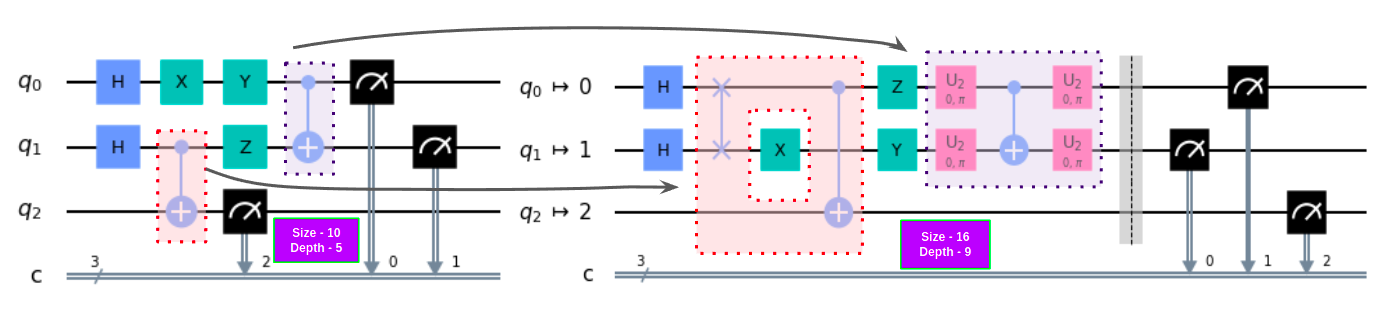
\includegraphics[width=\linewidth]{figures/intro/routing-transform.png}
    \caption{Transformation of a Quantum Circuit where non-local operations are scheduled to one implementable on the hardware (qubits 1 and 2 are not a local pair, 0 and 1, and 0 and 2 are). The decomposition of some gates is shown with arrows.}
\end{figure}

The value of the entire set of actions is largely dependent on the independent value of actions in the set, and the values added by the co-occurrance of small subsets of these actions, i.e. operations occuring on qubits significantly separated on hardware do not affect each other. This 

\subsection{qLEET: Variational Circuit Visualization}

\begin{figure}[H]
    \centering
    \hfill
    \begin{subfigure}[b]{0.45\linewidth}
        \centering
        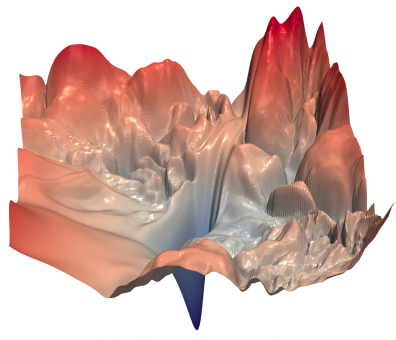
\includegraphics[width=0.7\textwidth]{figures/intro/landscape-rough.png}
        \caption{Loss Landscape without Skip Connections\label{fig:loss-landscape-rough}}
    \end{subfigure}
    \hfill
    \begin{subfigure}[b]{0.45\linewidth}
        \centering
        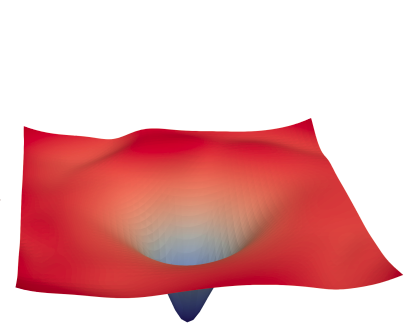
\includegraphics[width=0.7\textwidth]{figures/intro/landscape-smooth.png}
        \caption{Loss Landscape with Skip Connections\label{fig:loss-landscape-smooth}}
    \end{subfigure}
    \hfill
    \caption{The loss landscapes of neural networks with and without skip connections, as visualized by Li et. al.\cite{loss-landscapes}. The architectural decision of adding skip connections makes the feasibility of the optimization process a lot higher, to the extent visualizable on a 2-D random projection.}
    \label{fig:loss-landscape-neural-nets}
\end{figure}

\section{Thesis Layout}

\begin{itemize}
    \item[C1] This is the introductory chapter, which discusses the scope of the work carried out in this thesis in the context of developments in quantum computation, addresses the problems we are attempting to pose solutions to, and adds some motivation for the methods that we will develop in the following chapters.
    \item[C2] Here we presents a background in Quantum Computing and Reinforcement Learning which is requisite for understanding the motivations of the methods developed and the algorithms used in the remainder of this dissertation. We conclude this chapter by enlisting some ideas that we are going to use to address the problems posed in \ref{enum:problems-addressed-by-thesis}.
    \item[C3] As the first major contribution of this thesis, we present \textbf{qRoute: Qubit Routing using Graph Neural Network aided Monte Carlo Tree Search}, which is a reinforcement learning algorithm we propose for depth-minimized (used as a proxy for noise-mitigated) compilation. We discuss the problem of routing problem, discuss the specifics of our algorithm and associated neural architecture design.
    \item[C4] The other contribution of this thesis is \textbf{qLEET: Visualizing Loss Landscapes, Expressibility, Entangling power and Training Trajectories for Parameterized Quantum Circuits}, in which we present a way to analyze the properties of variational methods that can be implemented on present day quantum computers, and build a software framework for the same.
    \item[C5] We conclude with a summary of methods and results discussed in this thesis and the scope of extension of this work in the future.
\end{itemize}



%--------------------------------------------------------

\chapter{Quantum Computation and Reinforcement Learning}
\label{ch:background}
In this chapter, we introduce the basics of quantum computing and reinforcement learning. We start with discussing the basics of the mathematical and computational framework around quantum circuit design. We then describe some algorithms that give quantum computers their advantage.


\section{Quantum Computation}


\subsection{Qubits and Quantum Computation Model}

Quantum Computers store information as quantum bits, or qubits. These qubits can be evolved by operating on them with unitary operators, also called gates. The gate model of computation is rather familiar, following is a diagramatic illustration of the same:

\begin{figure}[ht]
    \centering
    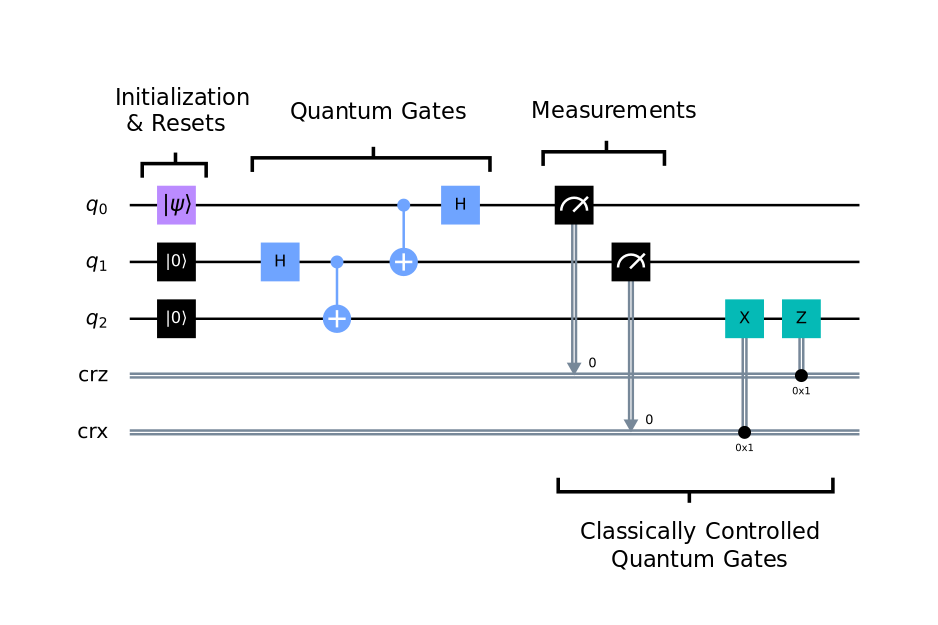
\includegraphics[width=0.8\linewidth]{figures/quantum/quantum_circuit_example.png}
    \caption{The image shows the parts of a typical quantum circuit, with 3 qubits represented by the wires and a set of gates applied to them, followed by measurement of those qubits.}
    \label{fig:quantum-circuit-example}
\end{figure}


A classical bit can be either 0 or 1. However, a qubit can live in any state inbetween 0 or 1, which is understood as being in a weighted superposition of the 0 and 1 states. So the state of a qubit 
\begin{equation}
    \ket{\psi} = \alpha \ket{0} + \beta \ket{1} = \begin{bmatrix}\alpha \\ \beta\end{bmatrix} \;\;\text{such that }\alpha^2 + \beta^2 = 1 \text{ and } \alpha, \beta \in \mathbb{C}
\end{equation}
where the normalization of probabilities forces. However this state of the qubit is not accessible to us, and we can only measure the qubit probabilistically, with probability of being $\ket{0}$ being $\alpha^2$ and that of $\ket{1}$ being $\beta^2$.

Each qubit, in addition to the superposition it is in also has a phase term, which is represented on the bloch-sphere \ref{fig:bloch-sphere} on the x-y plane. The phase doesn't affect the immediate measurement of the qubit, but can affect the resultant phase and superposition when some unitary operation is applied on the qubit.

\begin{figure}[H]
    \centering
    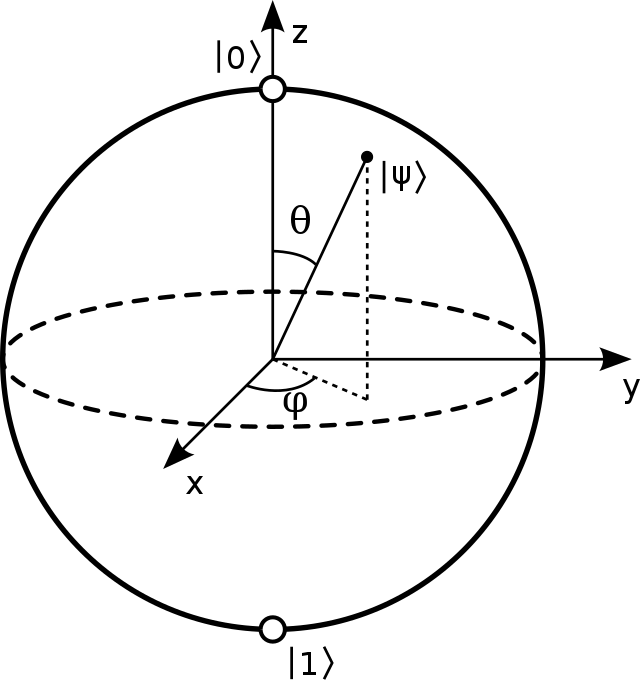
\includegraphics[width=0.5\linewidth]{figures/quantum/bloch_sphere.png}
    \caption{Bloch Sphere represents the state of a qubit $\ket{\psi}$. The pure states $\ket{0}$ and $\ket{1}$ are the vectors along the z-axis on the opposite poles. The angle along the x-y plane represents the phase of the qubits.}
    \label{fig:bloch-sphere}
\end{figure}


\subsection{Unitaries, Gates, and Entanglement}
\label{sec:background-unitary-gate-entanglement}

The state of a system of qubits can be modified by the application of unitary gates on those qubits.

\begin{figure}[h]
    \centering
    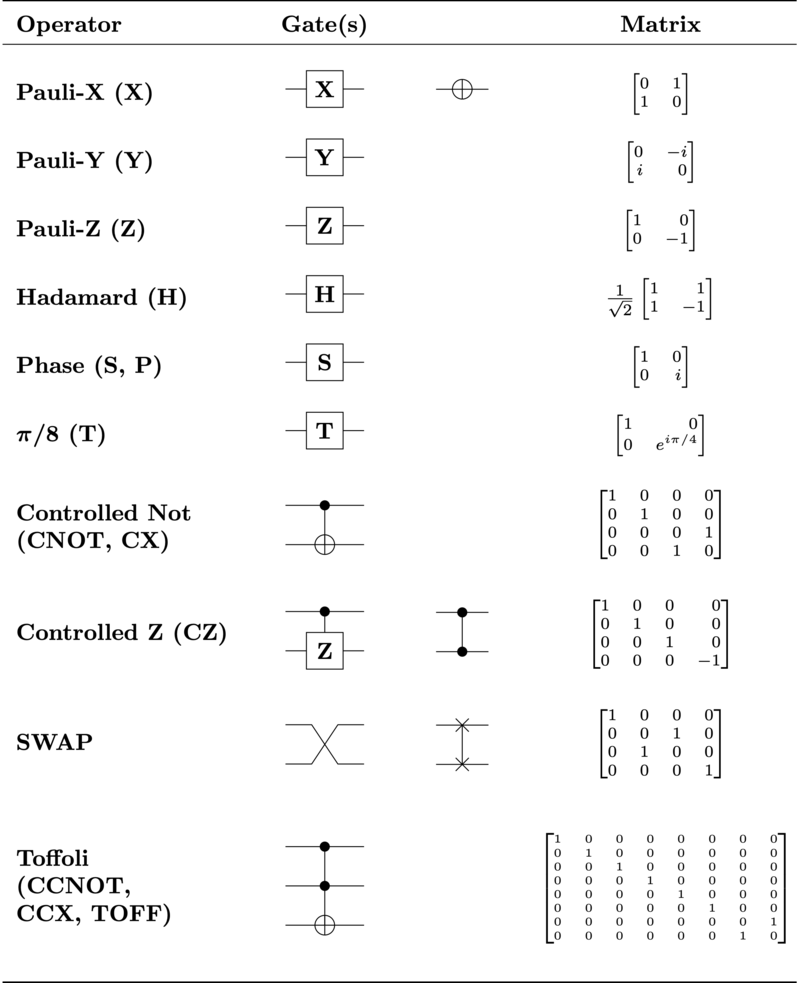
\includegraphics[width=0.7\linewidth]{figures/quantum/quantum_logic_gates.png}
    \caption{Popular logic gates along with their in-circuit representations and corresponding unitary matrices.}
    \label{fig:quantum-unitary-gates}
\end{figure}

Some multi-qubit gates introduce a property called entanglement. Examples of such gates are CNOT, CZ, etc. Once two qubits are ``entangled'' through some such operation like CNOT, their state cannot be written as a product of the individual states of the qubits, their are now linked in a way that the probability distribution of collapsing to either state along th measurement axis is not factorizable. 


\subsection{Density Matrices and Noise}

State preparation on a quantum computer is subject to noise, therefore there often exists some uncertainty in state of qubits on actual physical hardware. This uncertainty can be modelled as a classical probability distribution over the different quantum states that might have been prepared. Such a state is called a mixed state, as opposed to a pure state. Mixed states can be represented using Density matrices $\rho$, which are 2-D matrices with $2^n \times 2^n$ elements for $n$ qubits.
\begin{equation}
    \rho = \sum_{i} p_i \ket{x_i} \bra{x_i}
\end{equation}

Much like unitary operations on state vectors, the application of unitaries on density matrices can be represented through simple matrix multiplication:
\begin{equation}
    \mathcal{O} (\rho) = \sum_i p_i \mathcal{O}(\ket{x_i}) \mathcal{O}(\bra{x_i}) = \sum_i p_i U \ket{x_i} \bra{x_i} U^\dagger = U \rho U^\dagger
\end{equation}


\section{Quantum Algorithms}
\label{sec:quantum-algorithms}

Superposition and Entanglement together provide quantum computers with natural parallel processing power. While full access to this parallelism gets bottlenecked at the measurement layer since we can sample only one of the many states in weighted superposition, it is conceivable that for many an algorithm, this parallelism can result in a processing speed-up. A near-term goal with Quantum Computers is to achieve quantum supremacy, which is to solve a problem (possibly one of no practical use) that no classical computer can solve in a feasible amount of time. \cite{quantum-complexity-survey}

\begin{itemize}
    \item Grover Like - If a quantum algorithm succeeds with probability $p$, classically $1/p$ iterations are needed to succeed with constant certainty, whereas in the quantum setting using a technique called amplitude amplification, we can do the same in $O(1/\sqrt{p})$ iterations.
    \item Shor's Like - Algorithms which
    \item Hamiltonian Simulation - For several systems like the Quantum Harmonic Oscillator, or  
\end{itemize}


\subsection{Grover's Search}

Grover's search is an algorithm to search in a unordered list of size $n$ in $\sqrt{n}$ time proposed by Grover in 1996 \cite{grover-search-original}.

Since then, it has been the inspiration for many other algorithms, and many use it as a subroutine call, leading to a class of algorithms called amplitude amplification algorithms \cite{quantum-amplitude-amplification-algorithms}.

\paragraph*{The Problem:} Grover attacks the problem of unstructured search, where we have a list of $n$ elements in an any permutation and we have an oracle which marks each of these elements $1$, which is one of the results of the search procedure we wished to find, or as $0$ which is for those elements which were not one of those elements. We are told that the oracle only returns a value of $1$ for some $m$ of those elements, where $m << n$.

\paragraph*{Overview of the Algorithm:} Following is a brief explaination of how the Grover's algorithm operates:

\begin{enumerate}
    \item \textbf{Preparing the initial superposition of bitstrings:} The initial state should be the superposition of all elements in our search domain. Since these are the indices of the elements we are searching over, we can take this to be an equal superposition of all basis states, constructed by applying the hadamard gate over all qubits.
    \begin{equation}
        \ket{x} = \ket{s} = \frac{1}{\sqrt{n}} \sum_{i=1}^{n} \ket{b_i}
    \end{equation}

    \item \textbf{Application of a phase-kickback oracle:} For any input state $\ket{x}$, if it is a valid solution (i.e. $f(x) = 1$), then the oracle that bitstring with a negative phase. If $\ket{x}$ is not a basis state but rather is a superposition of states, then the oracle operates on each basis component of the state independently as shown in equation. \ref{eqn:grover-oracle}
    \begin{equation}\label{eqn:grover-oracle}
        \mathcal{O} \big(\ket{x} \big) = \mathcal{O}\bigg(\sum_i w_i(x) \ket{b_i} \bigg) = \sum_i w_i(x) \begin{cases}
            -\ket{b_i} & \text{if } f(b_i) = 1 \\
            \ket{b_i} & \text{if } f(b_i) = 0
        \end{cases}
    \end{equation}
    
    \item \textbf{Performing a reflection around the average amplitude:} Following the application of the oracle, we can apply a reflection around the mean amplitude of the superposition of all solutions via an application of the Diffuser operator.
    \begin{equation}
        \mathcal{D} \big(\ket{x} \big) = \big( 2 \ket{s}\bra{s} - 1 \big) \ket{x}
    \end{equation}
    Given that there are small number of solutions 
    \item \textbf{Repeat 2 steps above and measure the final state:} We iteratively apply the oracle and the diffuser circuit to take the present superposition closer and closer to the goal state. Measurement of this state along the computational basis gives us a bitstring, which with some constant probability is the solution $x$ such that $f(x) = 1$.
\end{enumerate}

\subsection{Shor's Algorithm}



\section{Variational Circuits}
\label{sec:variational-circuits}

In the previous section we have discussed purely quantum algorithms which do posess an advantage over their presently classical competitors, but need fault-tolerant quantum computers with a large number of qubits to be executed.

\subsection{Quantum Approximate Optimization Algorithm}
\label{sec:variational-circuits-qaoa}

\begin{figure}[ht]
    \centering
    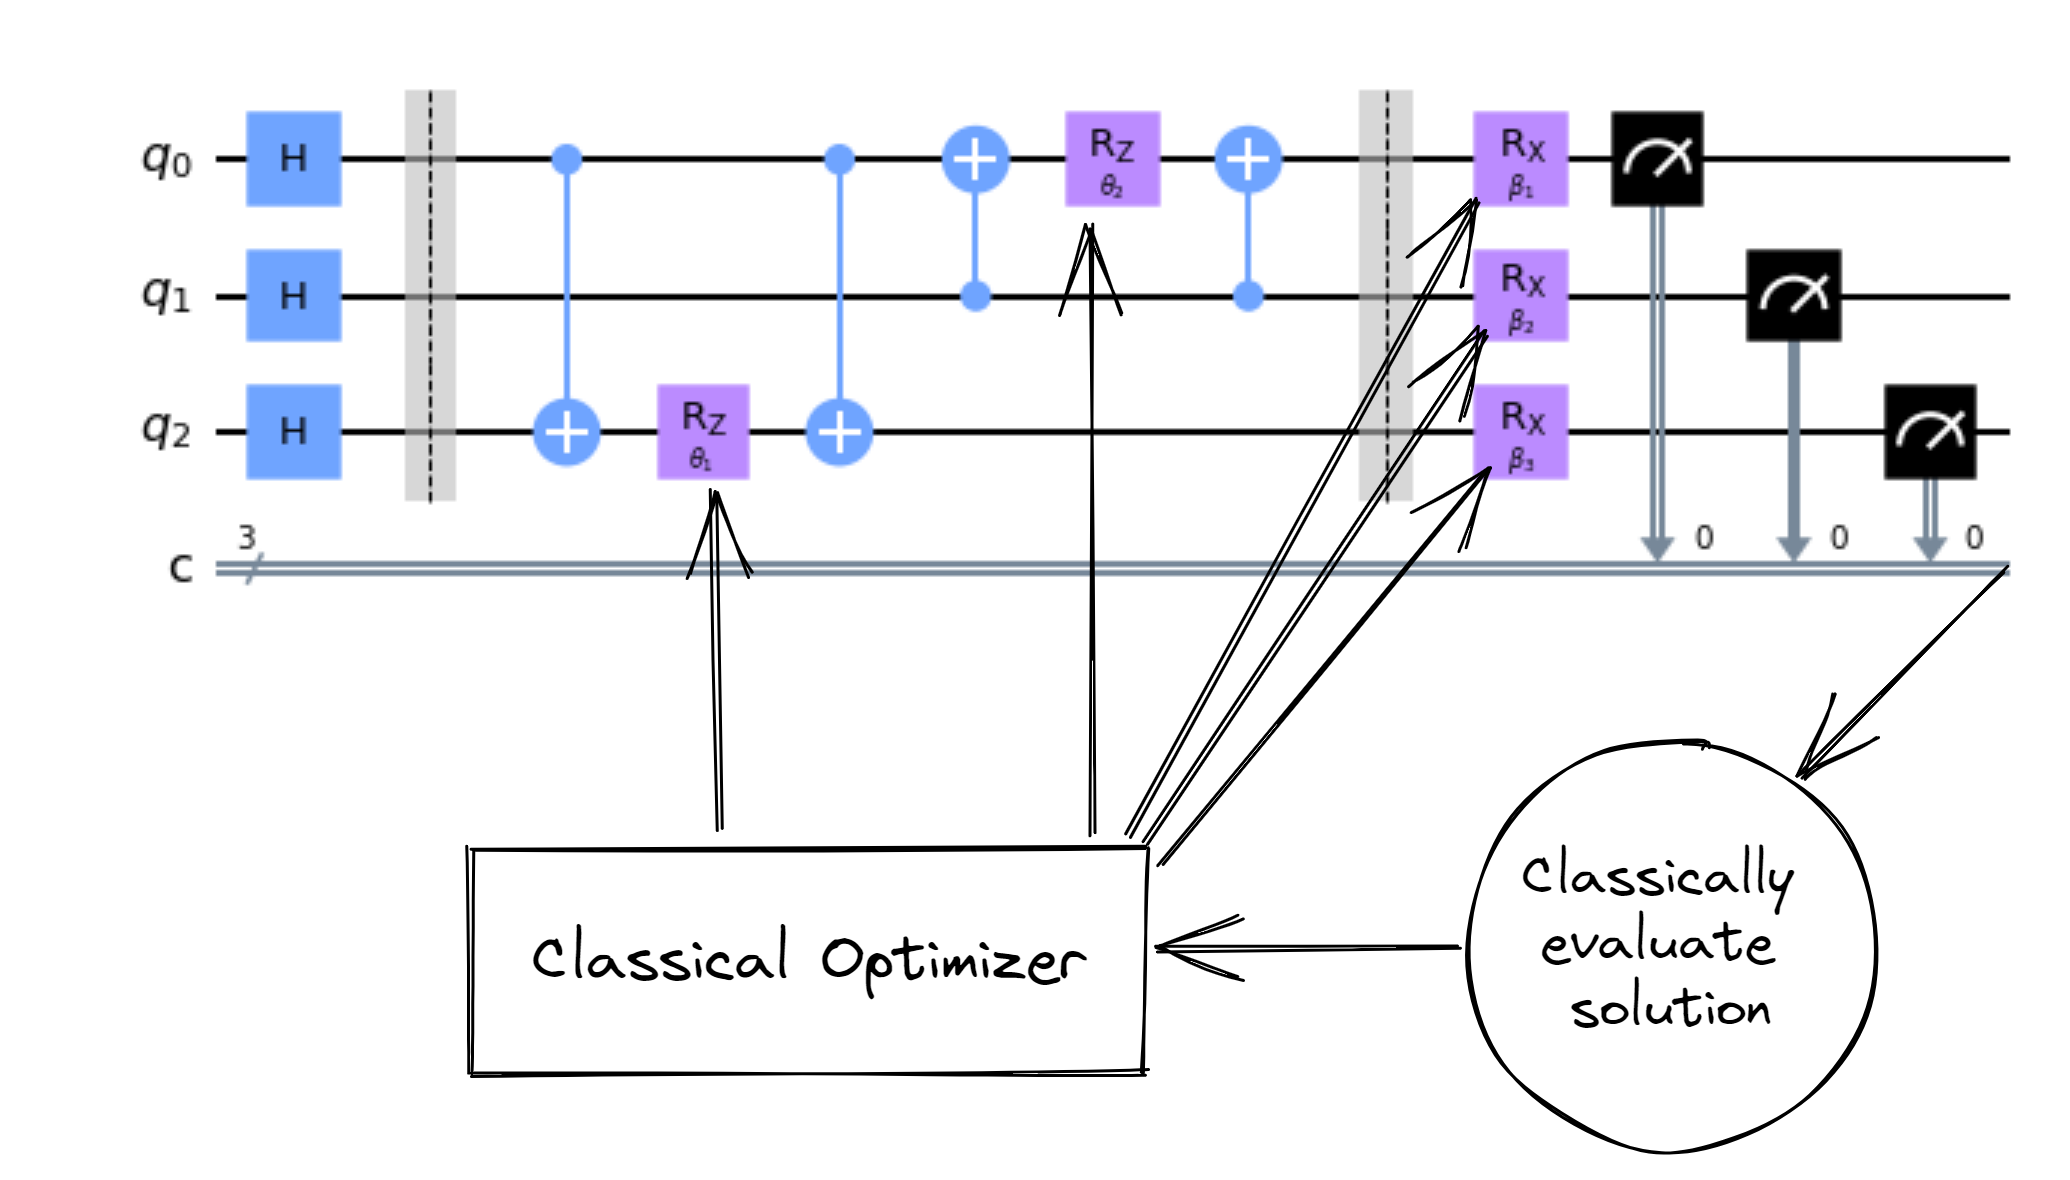
\includegraphics[width=0.7\linewidth]{figures/intro/qaoa-optimization.png}
    \caption[Variational Circuit for QAOA]{An example of a QAOA circuit with $p = 1$ blocks and generated to compute max-cut on a graph with 3-nodes and 2 edges between (0, 2) and (1, 0). The state generated by the circuit is parameterized in terms of the 5 parameters in the circuit. The output along the z-axis gets measured and is used to compute the classical loss value, i.e. the size of the max-cut given which set each node (represented by a qubit) belongs to. Finally, a classical optimizer is used to reduce the value of the loss function such that }
\end{figure}



\section{Reinforcement Learning}

\subsection{What is Reinforcement Learning}

Machine Learning and all associated sub-disciplines are motivated by the goal of achieving artificial general intelligence, that is being able to mimic the human mind and even surpass it's capacity to percieve, compute and actuate. The human mind deals with a veritable variety of problems differing greatly in their phrasing, in the solutions they admit, etc. Of this host of problem types, 

Deep Learning is an extremely powerful and popular one of these methods, which uses parameterized function approximators (aka. neural networks) to learn arbitrary functions directly from examples. We typically learn functions which take as input numerical data and associated structure (e.g. graphs) and produce one or many continuous-valued outputs (regression) or discrete-value outputs (classification). This has been employed with great success in computational chemistry, for instance, on predicting properties of molecules like solubility, smell, energy, etc. % Come up with more examples

Despite all their predictive power, these methods are limited in the set of problems they can solve. One limitation is our inability to provide a large number of labeled examples since running laboratory experiments or expensive in-silico simulations are often too time and resource-consuming. Another issue is that the output may not be a simple function of its inputs. For instance, when predicting molecular coordinates from molecular graphs, our outputs depend greatly on each other the position of one atom affects that of all others, and therefore a single step function cannot solve such a problem, an iterative approach to optimize these coordinates is required. In such cases where a problem is solved in many steps, there is no notion of the correct result after a single step, we can only score if the final result is produced by the composite of steps. All these problems necessitate a machine learning method which can produce outputs over several timesteps, and be able to reason about the correctness of its outputs based on rewards it may obtain at a different time in our process. This method is Reinforcement Learning. \cite{rl-intro-sutton-barto}


\subsubsection{Markov Decision Processes}

% What is environment, state, action

A Markov Decision Processes is any real or simulated process going on in time where each each decision follows the Markovian Property, i.e, any future state transitions or rewards are conditionally independent of the past states and actions given the present state the environment is in.

A Markov Decision Process (MDP) can be represented as a tuple $\braket{S, A, T_a(s, s^\prime), R_a(s, s^\prime)}$, where $S$ is the set of all states, $A$ is the set of all actions available from any given state, $T_a(s, s^\prime)$ is the transition model which represents the probability of going from a starting state $s$ to a next state $s^\prime$ given that the action $a$ was taken, and $R_a(s s^\prime)$ is the reward obtained when this transition is realized.

Reinforcement Learning is a method of solving Markov Decision Processes. For our problem to be solved by RL, we need to ensure that our formulation is Markovian, i.e. our state has enough information to, given the action, predict the probability of the next state and the associated reward.

\subsubsection{Value Function and Policy Function}

At every point in time, our agent has access to the state gets to choose an action, for which it gets a reward and the state of the simulation is updated. 
This process continues indefinitely until a terminal state is reached, i.e. one where no further progress needs to be made and no future rewards can be collected. This entire trajectory of states and actions together comprises an episode.

The agent maintains a function which is called it's \textbf{policy function} $\pi(s, a)$, which given the current state gives the probability of each action it can take from that state. Our agent is allowed to be stochastic for various practical and theoretical reasons, so the probability for more than one action in a given state is allowed to be non-zero. This is the function that we shall attempt to optimize while learning from our environment.

While acting according to any policy function, we can associate which each state what we call the \textbf{value function} $V_{\pi}(s)$, which represents the expected sum of rewards till the end of the episode obtainable by following the policy. The optimal policy function $\pi$ is that which leads to the maximum value function for the starting state.

Value-function of one state can be written in terms of that of others, and to compute these values over all the states we need to iteratively apply our updates.

\begin{equation}
    V(s) = \sum_{a \in A} \pi(s, a) \sum_{s^\prime} T_a(s, s^\prime) (V(s^\prime) + R_a(s, s^\prime))
\end{equation}

Instead of associating a value with each state, we can associate it with a state-action pair. This function is called the Q-function, and it carries equivalent information to the value function.
\begin{eqnarray}\label{eqn:defn-q-v-fn}
    Q(s, a) &=& \sum_{s^\prime} T_a(s, s^\prime) \bigg(R(s, s^\prime) + V(s^\prime) \bigg)\\
            &=& \sum_{s^\prime} T_a(s, s^\prime) \bigg(R(s, s^\prime) + \sum_{a \in A} \pi(s^\prime, a) Q(s^\prime, a)\bigg)
\end{eqnarray}

\subsection{Reinforcement Learning Algorithms}

In the following sections, we shall see three kinds of models:
\begin{itemize}
    \item Value Function Optimizers
    \item Policy Function Optimizers
    \item Actor-Critic Systems
    \item Planning based Reinforcement Learning
\end{itemize}


\subsubsection{Deep Q-Networks}

The first class of models attempt to approximate the value function. Assuming that our policy function will be that which is optimal, and assuming that our actions are deterministic (i.e. transition probabilities are 1 for the state we result in after an action and 0 otherwise), we can rewrite equation \ref{eqn:defn-q-fn} as:
\begin{eqnarray}\label{eqn:defn-q-fn}
    Q(s, a) \leftarrow R(s, s^\prime) + \max_{a \in A} Q(s^\prime, a)
\end{eqnarray}

For almost all problems in the real world, the state space is too large to maintain explicitly. Therefore we use a parameterized function $Q_{\theta}$, typically a neural network, to approximate the q-value from any given state-action pair.

The parameters $\theta$ can be updating using gradient based methods. The update operation in equation \ref{eqn:q-update} is 
\begin{equation}
    \label{eqn:q-update}
    \begin{split}
        \theta_{k+1} = \theta_k - \alpha \nabla_\theta \Bigg[\frac{1}{2} \bigg(Q_\theta(s, a) - \Big(R(s, a, s^\prime) + \gamma \max_{a^\prime} Q_{\theta_k}(s^\prime, a^\prime)  \Big) \bigg) \Bigg] \Bigg\vert_{\theta_k}
    \end{split}
\end{equation}

Several improvements to the training efficiency and stability to the DQN algorithm have been made, a few examples are the Double DQN by \cite{double-dqn}. These set of improvements put together have been analyzed by \cite{rainbow-dqn} under the name Rainbow DQN.

\subsubsection{Policy Function Approximators}

The policy function $\pi_\theta(s, a)$ gives the probability of each action given the state. In value function methods, we computed the policy by finding the action with the maximum expected value and assigning it a probability of 1 and other actions 0 for each state. When learning the policy directly, we use a stochastic policy instead, which makes the choice of actions smooth and optimizable.

\paragraph{Reasons to use policy gradients:}
\begin{enumerate}
    \item Learning value function may be much harder than learning the relative quality of actions, e.g. given the task of designing molecules with high solubility, and a procedure which keeps adding bonds iteratively, it can be very hard to predict the expected solubility of the molecule formed at the end of trajectories (value function), while predicting that adding a highly polar bond is more beneficial than adding non-polar ones (policy function).
    \item We might want to obtain a policy which is inherently stochastic, where policy based methods are the better choice. One example is when designing molecules with certain properties, we want a stochastic policy so that we can sample different molecules that optimize on the target property and then rank them based on synthetic ease or the such.
    \item Many a times, the action space is continuous or intractably large, and maximizing value over all actions is not feasible. Here we can only use policy based methods. Geometry optimization is one example, where the action is predicting the molecular coordinates of a single atom, which leads to a un-countably infinite sized action space.
\end{enumerate}

\paragraph{Method}:
To optimize our policy, we sample trajectories from our policy and increase the probability of actions in trajectories which high reward get increase, and those with lower reward decrease.

The utility of our policy is the expected reward under trajectories sampled from this policy, this is the quantity we wish to maximize over the parameters $\theta$. To perform this maximization, we compute $\nabla_\theta U(\theta)$ and update the parameter vector as $\theta \leftarrow \theta + \epsilon \nabla_\theta U(\theta)$. The gradient only depends on the gradient of the log of our policy function scaled by the rewards obtained along the trajectory, and very importantly does not depend on the true transition model. Equation \ref{eqn:policy-grad} follows from a mathematically involved derivation done in \cite{}.

\begin{equation}\label{eqn:policy-grad}
    \nabla_\theta U(\theta) \leftarrow \frac{1}{m} \sum_{i=1}^{m} \sum_{t=0}^{H-1} \nabla_\theta \log \pi_\theta (u_t^{(i)}|s_t^{(i)}) \Bigg(\sum_{k=t}^{H-1} R(s_k^{(i)}, u_k^{(i)}) - b(s_t^{(i)})\Bigg)
\end{equation}

\paragraph{Other Nuances}: Despite having the gradient that we need to update along, it's unclear what learning rate we should use to perform said update. Unlike in deep learning where the next iteration would correct if we overstep along the gradient, an overstep in our policy can lead to evaluation over an incorrect policy and can essentially wipe out all we have learnt till now. Trust Region policy optimizations (TRPO) by \cite{trpo} and Proximal Policy Optimizations (PPO) by \cite{ppo} are methods that address this. Furthermore, to increase sample efficiency, Direct Deterministic Policy Gradients (DDPG) by \cite{ddpg} and Soft Actor critic (SAC) \cite{sac} are used. These methods have not seen great application in chemistry but hold great promise given their popularity in other reinforcement learning sub-domains.

\subsubsection{Actor Critic Methods}

In equation \ref{eqn:policy-grad}, we are free to subtract a baseline value $b(s_t^{(i)})$ from the summed up rewards for each action, however this baseline should be independent of the action and can only depend on the state. Subtraction of this baseline leads to lower variance estimates in the value of actions. The network for each action now has to predict a quantity called the advantage, which represents the relative value of the actions and abstracts out the value of the state.
\begin{equation}\label{eqn:advantage}
    A(s, a) = Q(s, a) - V(s)
\end{equation}

This is implemented in practice using two networks, an actor network, which estimates the values of the actions, and a critic network, that estimates the resultant values of the states which we subtract as baseline from the rewards. These methods are often known to be stabler than their pure policy-gradient counterparts.

There are several variants on how the critic network and the explicit rollout together lead to the estimate of the value for each state, which have been discussed in detail by \cite{actor-critic-a2c, actor-critic-a3c, actor-critic-gae}

\subsubsection{Monte Carlo Tree Search}

When the transition model (next state and reward given action) is known, we can plan explicitly using a tree search. Since tree would grow combinatorially big (molecule generation via such means would have every possible molecule and it's substructure as a node in the tree), we use reinforcement learning to find out the most promising nodes. Monte Carlo Tree Search is one such method, which has gained prominence due to it's use in AlphaGo by \cite{mcts-alphago} to play Go and in AlphaZero by \cite{mcts-alphazero} to play Chess, Go, and other games with no human supervision during training. 

MCTS has been used in extensively chemistry wherever the exact transition model is known, in problems like Molecule Generation and Reaction path prediction. 



% Progress in computational techniques and speed is intimately tied to the furtherance of scientific inquiry. Over the past many decades, we have built computers that can simulate systems better and search for courses of action to modify the evolution of these systems to human advantage. In this endeavor, the manifold increase in computational speed and memory has helped us to date, but now that computational components have reached the size of atoms, we seem to be on the verge of meeting a hard limit. Therefore, we have started to look towards other paradigms to develop computers more suited to performing simulations of nature. Quantum computing, the idea of using the fundamental quantum nature of the universe to simulate itself but in much greater generality, has held the most promise.

% Richard Feynman said: “Nature isn't classical, dammit, and if you want to make a simulation of nature, you'd better make it quantum mechanical, and by golly it's a wonderful problem, because it doesn't look so easy.” \cite{feynman-quantum-simulating-physics}

% Though Quantum Computers are realizable even today, the devices in the present day are said to be a part of the Noisy Intermediate-Scale Quantum era (NISQ). Presently, the quantum bits and operations are noisy and lack the reliability to perform any computation infeasible on classical computers of the day.


%--------------------------------------------------------

\chapter{qRoute: Qubit Routing using Graph Neural Network aided Monte Carlo Tree Search}
\label{ch:qroute}
\section{\label{sec:abstract}Abstract}

Near-term quantum hardware can support two-qubit operations only on the qubits that can interact with each other. Therefore, to execute an arbitrary quantum circuit on the hardware, compilers have to first perform the task of qubit routing, i.e., to transform the quantum circuit either by inserting additional SWAP gates or by reversing existing CNOT gates to satisfy the connectivity constraints of the target topology.  The depth of the transformed quantum circuits is minimized by utilizing the Monte Carlo tree search (MCTS) to perform qubit routing by making it both construct each action and search over the space of all actions. It is aided in performing these tasks by a Graph neural network that evaluates the value function and action probabilities for each state. Along with this, we propose a new method of adding mutex-lock like variables in our state representation which helps factor in the parallelization of the scheduled operations, thereby pruning the depth of the output circuit. Overall, our procedure (referred to as QRoute) performs qubit routing in a hardware agnostic manner, and it outperforms other available qubit routing implementations on various circuit benchmarks.

{\smaller (Published in the Proceedings of AAAI Conferenence on Artificial Intelligence, 2022 \cite{self-qroute})}    
%\tableofcontents

\section{\label{sec:intro}Introduction}

The present-day quantum computers, more generally known as Noisy Intermediate-Scale quantum (NISQ) devices \cite{nisq_preskill} come in a variety of hardware architectures \cite{IBMQ, hardware_sycamore, hardware_rigetti_aspen, hardware_xanadu}, but there exist a few problems pervading across all of them. These problems constitute the poor quality of qubits, limited connectivity between qubits, and the absence of error-correction for noise-induced errors encountered during the execution of gate operations. These place a considerable restriction on the number of instructions that can be executed to perform useful quantum computation \cite{nisq_preskill}. Collectively these instructions can be realized as a sequential series of one or two-qubit gates that can be visualized more easily as a quantum circuit as shown in Fig. \ref{fig:orig_circ} \cite{others_childs}.

To execute an arbitrarily given quantum circuit on the target quantum hardware, a compiler routine must transform it to satisfy the connectivity constraints of the topology of the hardware \cite{qroute_tket}. These transformations usually include the addition of SWAP gates and the reversal of existing CNOT gates. This ensures that any non-local quantum operations are performed only between the qubits that are nearest-neighbors. This process of circuit transformation by a compiler routine for the target hardware is known as qubit routing \cite{qroute_tket}. The output instructions in the transformed quantum circuit should follow the connectivity constraints and essentially result in the same overall unitary evolution as the original circuit \cite{qroute_dqn2}.

In the context of NISQ hardware, this procedure is of extreme importance as the transformed circuit will, in general, have higher depth due to the insertion of extra SWAP gates. This overhead in the circuit depth becomes more prominent due to the high decoherence rates of the qubits and it becomes essential to find the most optimal and efficient strategy to minimize it \cite{qroute_tket, qroute_dqn1, qroute_dqn2}. In this chapter, we present a procedure that we refer to as \textit{QRoute}. We use Monte Carlo tree search (MCTS), which is a look-ahead search algorithm for finding optimal decisions in the decision space guided by a heuristic evaluation function \cite{mcts_bandit_1, mcts_bandit_2, mcts_uct}. We use it for explicitly searching the decision space for depth minimization and as a stable and performant machine learning setting. It is aided by a Graph neural network (GNN) \cite{nn_edge_conv}, with an architecture that is used to learn and evaluate the heuristic function that will help guide the MCTS.

%\textit{Structure}: In Section \ref{sec:qubit-routing}, we introduce the problem of qubit routing, the previous works that are done in the field, and show how our work differs from them. The methodology of the QRoute algorithm is described in Section \ref{sec:method}. In Section \ref{sec:results}, we benchmark the performance of our algorithm against other state-of-the-art quantum compilers. Finally, we discuss our results and  possible improvements in Section \ref{sec:discussion-conclusion}.

\begin{figure}
    \centering
    \hfill
    \begin{subfigure}[b]{0.30\linewidth}
        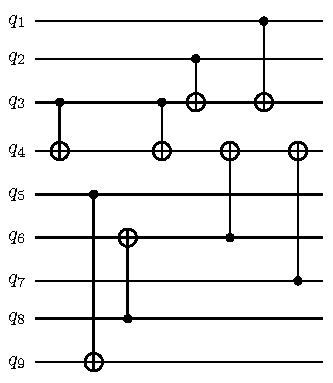
\includegraphics[width=\textwidth]{figures/qroute/orig_circ.pdf}
        \caption{Quantum circuit\label{fig:orig_circ}}
    \end{subfigure}
    \hfill
    \begin{subfigure}[b]{0.30\linewidth}
        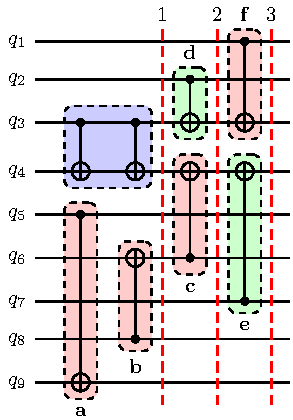
\includegraphics[width=0.85\textwidth]{figures/qroute/sliced_circ.pdf}
        \caption{Decomposed circuit\label{fig:sliced_circ}}
    \end{subfigure}
    \hfill
    \begin{subfigure}[b]{0.35\linewidth}
        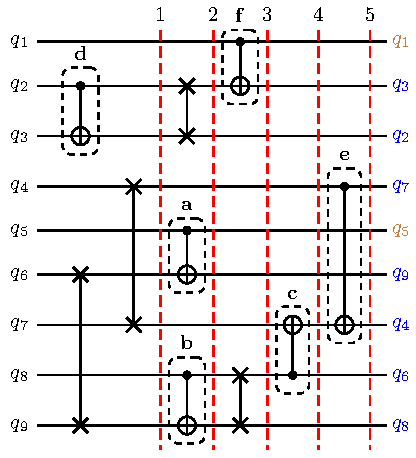
\includegraphics[width=\textwidth]{figures/qroute/transformed_circ.pdf}
        \caption{Decomposed transformed circuit\label{fig:transformed_circ}}
    \end{subfigure}
    \hfill
    \caption[Topologies of Quantum Computing hardware qRoute is tested on]{An example of qubit routing on a quantum circuit for 3$\times$3 grid architecture (Figure \ref{fig:3-3-arch}). (a) For simplicity, the original quantum circuit consists only of two-qubit gate operations. (b) Decomposition of the original quantum circuit into series of slices such that all the instructions present in a slice can be executed in parallel. The two-qubit gate operations: $\{d,e\}$ (green) comply with the topology of the grid architecture whereas the operations: $\{a, b, c, f\}$ (red) do not comply with the topology (and therefore cannot be performed). Note that the successive two-qubit gate operations on $q_3\rightarrow q_4$ (blue) are redundant and are not considered while routing. (c) Decomposition of the transformed quantum circuit we get after qubit routing. Four additional SWAP gates are added that increased the circuit depth to $5$, i.e., an overhead circuit depth of $2$. The final qubit labels are represented at the end right side of the circuit. The qubits that are not moved (or swapped) are shown in brown ($\{q_1, q_5\}$), while the rest of them are shown in blue.}
    %Note that the overall unitary operation performed by the circuit is preserved despite the changes in the order of two-qubit gate operations.}
    \label{fig:routing-example}
\end{figure}

\begin{figure}
    \centering
    \begin{subfigure}[b]{0.4\linewidth}
        \centering
        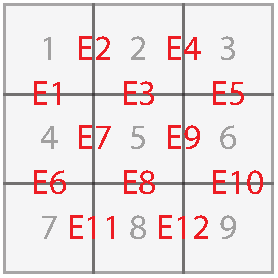
\includegraphics[width=0.5\linewidth]{figures/qroute/Grid-device.pdf}
        \caption{3$\times$3 grid architecture with edges (i.e. neighboring qubits) labelled \label{fig:3-3-arch}}
    \end{subfigure}
    \begin{subfigure}[b]{0.5\linewidth}
        \centering
        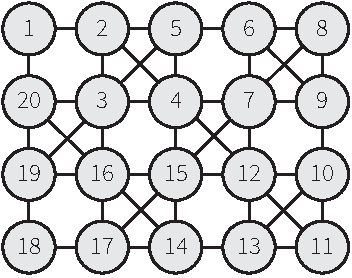
\includegraphics[width=0.5\linewidth]{figures/qroute/QX20-device.pdf}
        \caption{IBMQX-20 architecture represented as a graph}
    \end{subfigure}
    \caption{Examples of qubit connectivity graphs for some common quantum architectures}
    \label{fig:topology-example}
\end{figure}

\section{\label{sec:qubit-routing}Qubit Routing}
In this section, we begin by defining the problem of qubit routing formally and discussing the work done previously in the field.

\subsection{\label{sec:intro-defn}Describing the Problem}
The topology of quantum hardware can be visualized as a qubit connectivity graph (Fig. \ref{fig:topology-example}). Each node in this graph would correspond to a physical qubit which in turn might correspond to a logical qubit. The quantum instruction set, which is also referred to as quantum circuit (Fig. \ref{fig:orig_circ}), is a sequential series of single-qubit and two-qubit gate operations that act on the logical qubits. The two-qubit gates such as CNOT can only be performed between two logical qubits iff there exists an edge between the nodes that correspond to the physical qubits, \cite{qroute_dqn1}. This edge could be either unidirectional or bidirectional, i.e., CNOT can be performed either in one direction or in both directions. In this work, we consider only the bidirectional case, while noting that the direction of a CNOT gate can be reversed by sandwiching it between a pair of Hadamard gates acting on both control and target qubits \cite{utk_equiv_circuits}. 

Given a target hardware topology $\mathcal{D}$ and a quantum circuit $\mathcal{C}$, the task of qubit routing refers to transforming this quantum circuit by adding a series of SWAP gates such that all its gate operations then satisfy the connectivity constraints of the target topology (Fig. \ref{fig:transformed_circ}). Formally, for a routing algorithm $\textrm{R}$, we can represent this process as follows:
\begin{equation}
\textrm{R}(\mathcal{C},\ \mathcal{D}) \rightarrow \mathcal{C}^{\prime}
\end{equation}
Depth of $\mathcal{C}^{\prime}$ (transformed quantum circuit) will, in general, be more than that of the original circuit due to the insertion of additional SWAP gates. This comes from the definition of the term \textit{depth} in the context of quantum circuits. This can be understood by decomposing a quantum circuit into series of individual slices, each of which contains a group of gate operations that have no overlapping qubits, i.e., all the instructions present in a slice can be executed in parallel (Fig. \ref{fig:sliced_circ}). The depth of the quantum circuit then refers to the minimum number of such slices the circuit can be decomposed into, i.e., the minimum amount of parallel executions needed to execute the circuit. The goal is to minimize the overhead depth of the transformed circuit with respect to the original circuit.

This goal involves solving two subsequent problems of (i) qubit allocation, which refers to the mapping of program qubits to logic qubits, and (ii) qubit movement, which refers to routing qubits between different locations such that interaction can be made possible \cite{utk_qubit_noise}. In this work, we focus on the latter problem of qubit movement only and refer to it as qubit routing. However, it should be  noted that qubit allocation is also an important problem and it can play an important role in minimizing the effort needed to perform qubit movement.



\subsection{\label{sec:intro-related}Related Work}

The first major attraction for solving the qubit routing problem was the competition organized by IBM in 2018 to find the best routing algorithm. This competition was won by \cite{zulehner2018mapping}, for developing a Computer Aided Design-based (CAD) routing strategy. Since then, this problem has been presented in many different ways. These include graph-based architecture-agnostic solution by \cite{qroute_tket}, showing equivalence to the travelling salesman problem by \cite{paler_torus}, machine learning based methods by \cite{paler_ml}, and heuristic approaches by \cite{review-1}, \cite{review-2}, \cite{review-3}, etc. A reinforcement learning in a combinatorial action space solution was proposed by \cite{qroute_dqn1}, which suggested used simulated annealing to search through the combinatorial action space, aided by a Feed-Forward neural network to judge the long-term expected depth. This was further extended to use Double Deep Q-learning and prioritized experience replay by \cite{qroute_dqn2}. 

Recently, Monte Carlo tree search (MCTS), a popular reinforcement learning algorithm \cite{mcts_survey} previously proven successful in a variety of domains like playing puzzle games such as Chess and Go \cite{mcts_alphago}, and was used by \cite{qroute_mcts} to develop a qubit routing solution. 
%However, they used MCTS in the context of minimizing the total volume of quantum circuits (i.e., the number of gates ignoring the parallelization).

% \begin{figure*}[t]
%     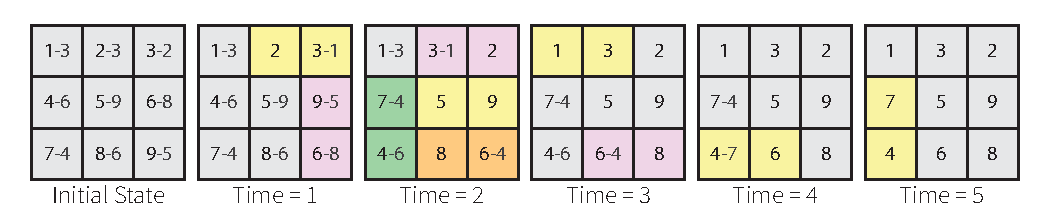
\includegraphics[width=\linewidth]{figures/qroute/Evolution.pdf}
% 	\caption{\label{fig:routing-progress}Routing progress for 3$\times$3 grid architecture while for the quantum circuit in Fig. \ref{fig:orig_circ}. Initial state shows the gate scheduled on each qubit which gets executed as control and target qubit adjacent to each other via SWAPs (shown in green and purple). The final state (at time=$5$) shows the final evolved qubit mapping. Here, each state (at time step=$t$) corresponds to the $t^{\rm{th}}$ time slice in Fig. \ref{fig:transformed_circ}}
% \end{figure*}

\subsection{\label{sec:intro-contribution}Our Contributions}

Our work demonstrates the use of MCTS on the task of Qubit Routing and presents state of the art results. Following are the novelties of this approach:

\begin{itemize}
    \item We use an array of mutex locks to represent the current state of parallelization, helping to reduce the depth of the circuits instead of the total quantum volume, in contrast to previous use of MCTS for qubit routing in \cite{qroute_mcts}.
    \item The actions in each timestep (layer of the output circuit) belong to a innumerably large action space. We phrase the construction of such actions as a Markov decision process, making the training stabler and the results better, particularly at larger circuit sizes, than those obtained by performing simulated annealing to search in such action spaces \cite{qroute_dqn1, qroute_dqn2}. Such approach should be applicable to other problems of a similar nature.
    \item Graph neural networks are used as an improved architecture to help guide the tree search.
\end{itemize}

Finally, we provide a simple python package containing the implementation of QRoute, together with  an easy interface for trying out different neural net architectures, combining algorithms, reward structures, etc.

\begin{figure}[ht]
    \centering
    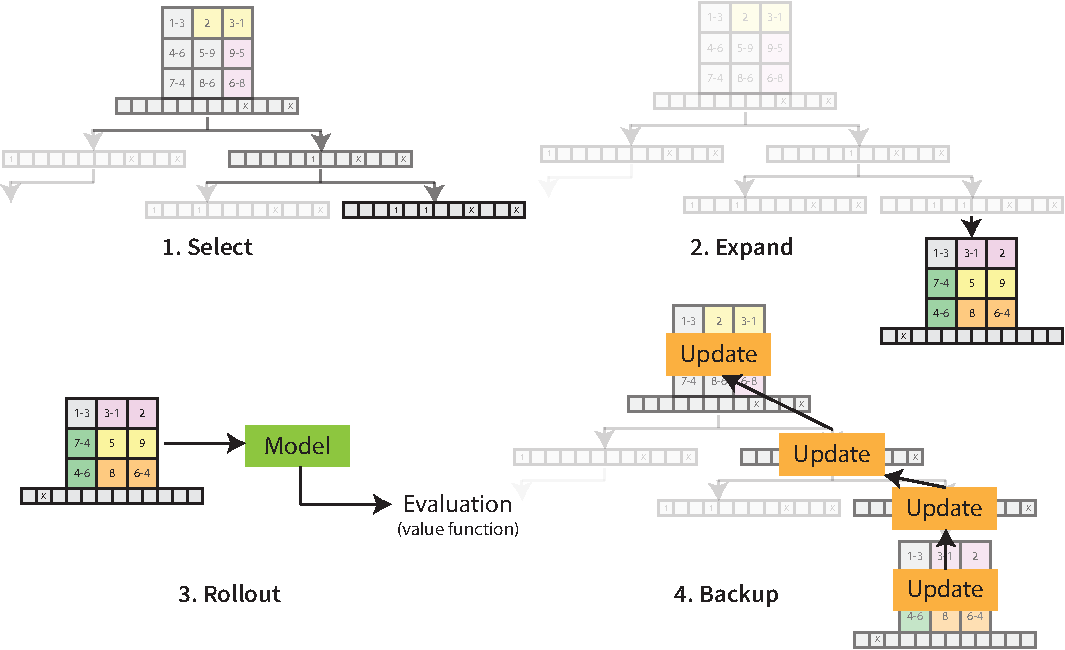
\includegraphics[width=\linewidth]{figures/qroute/Search.pdf}
    \caption[Visualization of steps in Monte Carlo Tree Search]{
        Iteration of a Monte Carlo tree search: (i) select - recursively choosing a node in the search tree for exploration using a selection criteria, (ii) expand - expanding the tree using the available actions if an unexplored leaf node is selected, (iii) rollout - estimating long term reward using a neural network for the action-state pair for the new node added to search tree, and (iv) backup - propagating reward value from the leaf nodes upwards to update the evaluations of its ancestors.}
    \label{fig:mcts-explainer}
\end{figure}


\newtheorem{defn}{Definition}[section]

\section{\label{sec:method}Method}

The QRoute algorithm takes in an input circuit and an injective map, $\mathcal{M}: Q \rightarrow N$, from logical qubits to nodes (physical qubits). Iteratively, over multiple timesteps, it tries to schedule the gate operations that are present in the input circuit onto the target hardware. To do so, from the set of unscheduled gate operations, $\mathcal{P}$, it takes all the current operations, which are the first unscheduled operation for both the qubits that they act on, and tries to make them into local operations, which are those two-qubit operations that involve qubits that are mapped to nodes connected on the target hardware.

In every timestep $t$, QRoute starts by greedily scheduling all the operations that are both current and local in $\mathcal{P}$. To evolve $\mathcal{M}$, it then performs a Monte Carlo tree search (MCTS) to find an optimal set of SWAPs by the evaluation metrics described in the Section \ref{sec:method-mcts} such that all operations in the current timestep put together form a parallelizable set, i.e., a set of local operations such that no two operations in the set act on the same qubit. The number of states we can encounter in the action space explodes exponentially with the depth of our search, therefore an explicit search till the circuit is done compiling is not possible. Therefore we cut short our search at some shallow intermediate state, and use a neural network to get its heuristic evaluation.


The following subsections describe in greater detail the working of the search and the heuristic evaluation.

\subsection{\label{sec:method-state} State and Action Space}

\begin{defn}[State]
    It captures entire specification of the state of compilation at some timestep t. Abstractly, it is described as:
    \begin{equation}
        s_{t} = (\mathcal{D}, \ \mathcal{M}_{t},\ \mathcal{P}_{t},\ \mathcal{L}_{t})
    \end{equation}

    where, $\mathcal{D}$ is the topology of target hardware, and $\mathcal{M}_t$ and $\mathcal{P}_t$ represents the current values of $\mathcal{M}$ and $\mathcal{P}$ respectively. $\mathcal{L}_{t}$ is the set of nodes that are locked by the gate operations from the previous timestep and therefore cannot be operated in the current timestep. 
\end{defn}


\begin{defn}[Action]
    It is a set of SWAP gates (represented by the pair of qubits it acts on) such that all gates are local, and its union with the set of operations that were scheduled in the same timestep forms a parallelizable set.
\end{defn}

We are performing a tree search over state-action pairs. Since the number of actions that can be taken at any timestep is exponential in the number of connections on the hardware, we are forced to build a single action up, step-by-step. 

\begin{defn}[Move]
    It is a single step in a search procedure which either builds up the action or applies it to the current state. Moves are of the following two types:
    \begin{enumerate}
        \item SWAP($n_1$, $n_2$): Inserts a new SWAP on nodes $n_1$ and $n_2$ into the action set. Such an insertion is only possible if the operation is local and resulting set of operations for the timestep form a parallel set.
        \item COMMIT: Finishes the construction of the action set for that timestep. It also uses the action formed until now to update the state $s_t$ (schedules the SWAP gates on the hardware), and resets the action set for the next step.
    \end{enumerate}
\end{defn}

In reality, different gate operations take different counts of timesteps for execution. For example, if a hardware requires SWAP gate to be broken down into CNOT gates, then it would take three timesteps for complete execution \cite{utk_equiv_circuits}. This means, operations which are being scheduled must maintain mutual exclusivity with other other operations over the nodes which participates in them. This is essential to minimizing the depth of the circuit since it models paralleizability of operations.

However, constructing a parallelizable set and representing the state of parallelization to our heuristic evaluator is a challenge. But an analogy can be drawn here to the nodes being thought of as ``resources" that cannot be shared, and the operations as ``consumers" \cite{mutex_dijkstra}. This motivates us to propose the use of Mutex Locks for this purpose. These will lock a node until a scheduled gate operation involving that node executes completely. Therefore, this allows our framework to naturally handle different types of operations which take different amounts of time to complete.

% On some hardware, SWAP gates are not primitive and get decomposed to three CNOT gates. Therefore they are thrice as slow as other primitive gates. This is easily modelled by keeping the mutex locks for those nodes locked for three timesteps. Therefore, this allows our framework to naturally handle different types of operations which take different amounts of time to complete.

For every state-action pair, the application of a feasible move $m$ on it will result in a new state-action pair: $(s,a) \xrightarrow[]{m} (s^\prime,a^\prime)$. This is a formulation of the problem of search as a Markov Decision Process. Associated with each such state-action-move tuple $((s, a), m)$, we maintain two additional values that are used by MCTS:

\begin{enumerate}
\item \textit{N-value} - The number of times we have taken the said move $m$ from said state-action pair $(s,a)$.
\item \textit{Q-value} - Given a reward function $\mathcal{R}$, it is the average long-term reward expected after taking said move $m$ over all iterations of the search. (Future rewards are discounted by a factor $\gamma$)

\begin{equation}
\begin{split}
    Q((s,a), m) =&\ \mathcal{R}((s,a), m)\ + \\ & \gamma \frac{\sum_{m^\prime} N((s^\prime, a^\prime), m^\prime) \cdot Q((s^\prime, a^\prime), m^\prime)}{\sum_{m^\prime} N((s^\prime, a^\prime), m^\prime)}
\end{split}
\end{equation}

\end{enumerate}

\begin{figure*}[th]
\centering
    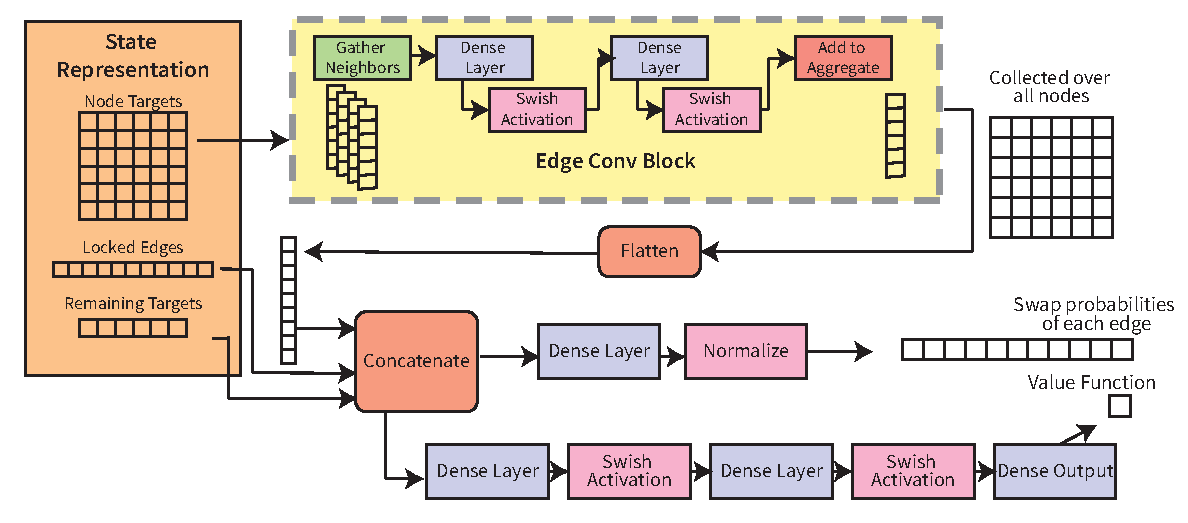
\includegraphics[width=\textwidth]{figures/qroute/Architecture.pdf}
    \caption[Graph neural network architecture that approximates value and policy function]{\label{fig:network-architecture}
     Graph neural network architecture that approximates the value function and the policy function.}
     %The $state$ object (orange), shown on the far left, is provided as an input. The edge convolution block (yellow) extracts the features from the input object, collects them, flattens them, and concatenates them with the rest of the input for further processing. Here, the network diverges into two segments, one called the value head, which gives a scalar output representing the quality of the state, and another policy head, which provides the probability distribution over the best action from this state.}
\end{figure*}

\subsection{\label{sec:method-mcts} Monte Carlo Tree Search}

Monte Carlo tree search progresses iteratively by executing its four phases: select, expand, rollout, and backup as illustrated in Fig. \ref{fig:mcts-explainer}. In each iteration, it begins traversing down the existing search tree by selecting the node with the maximum UCT value (Eq. \ref{eq:uct}) at each level. During this traversal, whenever it encounters a leaf node, it expands the tree by choosing a move $m$ from that leaf node. Then, it estimates the scalar evaluation for the new state-action pair and backpropagates it up the tree to update evaluations of its ancestors.

To build an optimal action set, we would want to select the move $m$ with the maximum true Q-value. But since true Q-values are intractably expensive to compute, we can only approximate the Q-values through efficient exploration. We use the Upper Confidence Bound on Trees (UCT) objective \cite{mcts_uct} to balance exploration and exploitation as we traverse through the search tree. Moreover, as this problem results in a highly asymmetric tree, since some move block a lot of other moves, while others block fewer moves, we use the formulation of UCT adapted for asymmetric trees \cite{mcts_assymetric}:

\begin{equation}\label{eq:uct}
\begin{split}
    \textrm{UCT}((s,a), m) =&\ Q((s,a), m)\ + \\ & c \frac{\sqrt{\sum_m N((s,a), m)}}{N((s,a), m)} \times p(m \vert (s,a))
\end{split}
\end{equation}

Here, the value $p(m | (s,a))$ is the prior policy function, which is obtained by adding a Dirichlet noise to the policy output of the neural network \cite{mcts_alphazero}. As MCTS continues probing the action space, it gets a better estimate of the true values of the actions. This means that it acts as a policy enhancement function whose output policy (Eq. \ref{eq:mcts_output}) can be used to train the neural network's prior ($\pi$), and the average Q-value computed can be used to train its scalar evaluation (Eq. \ref{eq:train_nn}).

\begin{equation}\label{eq:mcts_output}
    \pi(m | (s,a)) \propto N((s, a), m))
\end{equation}

\begin{equation}\label{eq:train_nn}
    \mathcal{V}((s,a)) = \frac{\sum_{m} Q((s,a), m)}{\sum_{m} N((s,a), m)}
\end{equation}



The details of how MCTS progresses have been elaborated in the supplementary. Once it gets terminated, i.e., the search gets completed, we go down the tree selecting the child with the maximum Q-value at each step until a COMMIT action is found, we use the action set of the selected state-action pair to schedule SWAPs for the current timestep, and we re-root the tree at the child node of the COMMIT action to prepare for the next timestep.

\subsection{\label{sec:method-model}Neural Network Architecture}

Each iteration of the MCTS requires evaluation of Q-values for a newly encountered state-action pair. But these values are impossible to be computed exactly since it would involve an intractable number of iterations in exploring and expanding the complete search tree. Therefore, it is favorable to heuristically evaluate the expected long-term reward from the state-action pair using a Neural Network, as it acts as an excellent function approximator that can learn the symmetries and general rules inherent to the system.

So, once the MCTS sends a state-action pair to the evaluator, it begins by committing the action to the state and getting the resultant state. We then generate the following featurized representation of this state and pass this representation through the neural-network architecture as shown in Fig. \ref{fig:network-architecture}.

\begin{enumerate}
    \item \textit{Node Targets} - It is a square boolean matrix whose rows and columns correspond to the nodes on a target device. An element $(i, j)$ is true iff some logical qubits $q_x$ and $q_y$ are currently mapped to nodes $i$ and $j$ respectively, such that ($q_x$, $q_y$) is the first unscheduled operation that $q_x$ partakes in.
    \item \textit{Locked Edges} - It is a set of edges (pairs of connected nodes) that are still locked due to either of its qubits being involved in an operation in the current timestep or another longer operation that hasn't yet terminated from the previous timesteps.
    \item \textit{Remaining targets} - It is a list of the number of gate-operations that are yet to be scheduled for each logical qubit. 
\end{enumerate}

% \begin{enumerate}
%     \item The \textbf{target node} for some node $n_1$ is a node $n_2$, such that if qubit $q_1$ is currently mapped to $n_1$ and $q_2$ is mapped to $n_2$, then the operation ($q_1$, $q_2$) is the first operation in the input circuit that $q_1$ partakes in, which has not already been scheduled.
%     \item The number of \textbf{remaining targets} for some qubit $q$ is the number of operations involving it which are yet to be scheduled.
%     \item \textbf{Locked edges} is the set of edges (pairs of connected qubits) which are still locked due to either of it's qubits being involved in an operation in the current timestep or a longer operation that hasn't yet terminated from the previous timestep.
% \end{enumerate}

The SWAP operations each qubit would partake in depends primarily on its target node, and on those of the nodes in its neighborhood that might be competing for the same resources. It seems reasonable that we can use a Graph Neural Network with the device topology graph for its connectivity since the decision of the optimal SWAP action for some node is largely affected by other nodes in its physical neighborhood. Therefore, our architecture includes an edge-convolution block \cite{nn_edge_conv}, followed by some fully-connected layers with Swish \cite{nn_swish} activations for the policy and value heads. The value function and the policy function computed from this neural network are returned back to the MCTS.



\section{\label{sec:results}Results}
We compare QRoute against the routing algorithms from other state-of-the-art frameworks on various circuit benchmarks: (i) Qiskit and its three variants \cite{comp_qiskit}: (a) basic, (b) stochastic, and (c) sabre, (ii) Deep-Q-Networks (DQN) from \cite{qroute_dqn2}, (iii) Cirq \cite{comp_cirq}, and (iv) t$\ket{\text{ket}}$ from Cambridge Quantum Computing (CQC) \cite{comp_pytket}. 
% The routing algorithm in t$\ket{\text{ket}}$ uses BRIDGE gates along with SWAP gates and
Qiskit's transpiler uses gate commutation rules while perform qubit routing. This strategy is shown to be advantageous in achieving lower circuit depths \cite{bridge_gate} but was disabled in our simulations to have a fair comparison. The results for DQN shown are adapted from the data provided by the authors \cite{qroute_dqn2}.

\begin{figure}[t]
    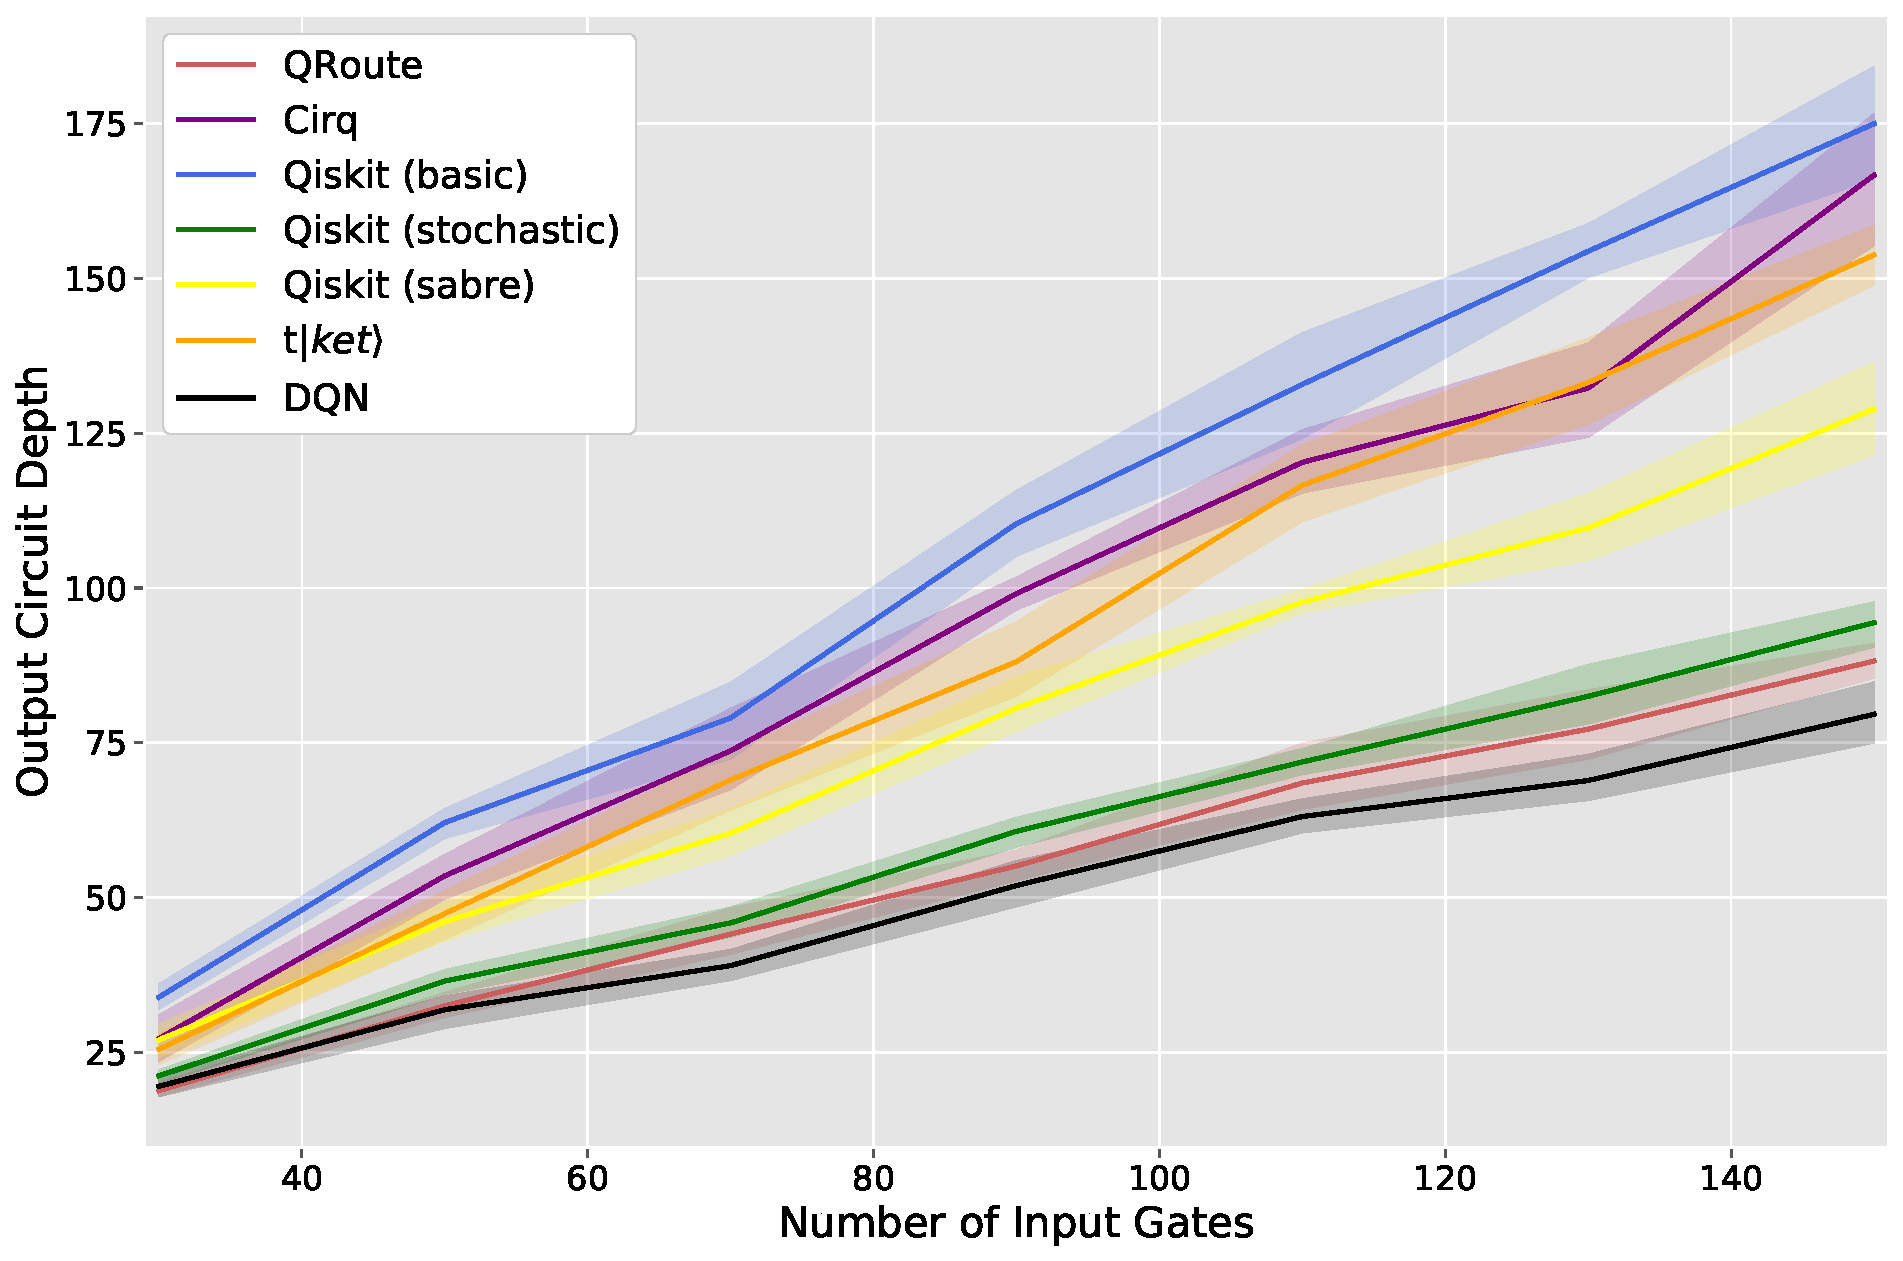
\includegraphics[width=\linewidth]{figures/qroute/random_benchmark.pdf}
    \caption[qRoute Results on randomly generated circuits]{\label{fig:results-random}
        Comparative performance of routing algorithms on random circuits as a function of the number of two-qubit operations in the circuit.}
\end{figure}

\subsection{\label{sec:results-random}Random Test Circuits}

The first benchmark for comparing our performance comprises of random circuits. These circuits are generated on the fly and initialized with the same number of qubits as there are nodes on the device. Then two-qubit gates are put between any pair of qubits chosen at random. In our simulations, the number of such gates is varied from 30 to 150 and the results for assessing performance of different frameworks are given in Fig. \ref{fig:results-random}. The experiments were repeated 10 times on each circuit size, and final results were aggregated over this repetition. 


Amongst the frameworks compared, QRoute ranks a very close second only to Deep-Q-Network guided simulated annealer (DQN). Nevertheless, QRoute still does consistently better than all the other major frameworks: Qiskit, Cirq and t$\ket{\text{ket}}$, and it scales well when we increase the number of layers and the layer density in the input circuit. QRoute shows equivalent performance to DQN on smaller circuits, and on the larger circuits it outputs depths which are on average $\leq 4$ layers more than those of DQN. Some part of this can be attributed to MCTS, in its limited depth search, choosing the worse of two moves with very close Q-values, resulting in the scheduling of some unnecessary SWAP operations.


\subsection{\label{sec:results-small}Small Realistic Circuits}

Next we test on the set of all circuits which use 100 or less gates from the IBM-Q realistic quantum circuit dataset used by \cite{data_realistic}. The comparative performance of all routing frameworks has been shown by plotting the depths of the output circuits summed over all the circuits in the test set in Fig. \ref{fig:results-small}. Since the lack of a good initial qubit allocation becomes a significant problem for all pure routing algorithms on small circuits, we have benchmarked QRoute on this dataset from three trials with different initial allocations.

The model presented herein has the best performance on this dataset. We also compare the best result from a pool of all routers including QRoute against that of another pool of the same routers but excluding QRoute. The pool including QRoute gives on average $2.5\%$ lower circuit depth, indicating that there is a significant number of circuits where QRoute is the best routing method available.

\begin{figure}[t]
    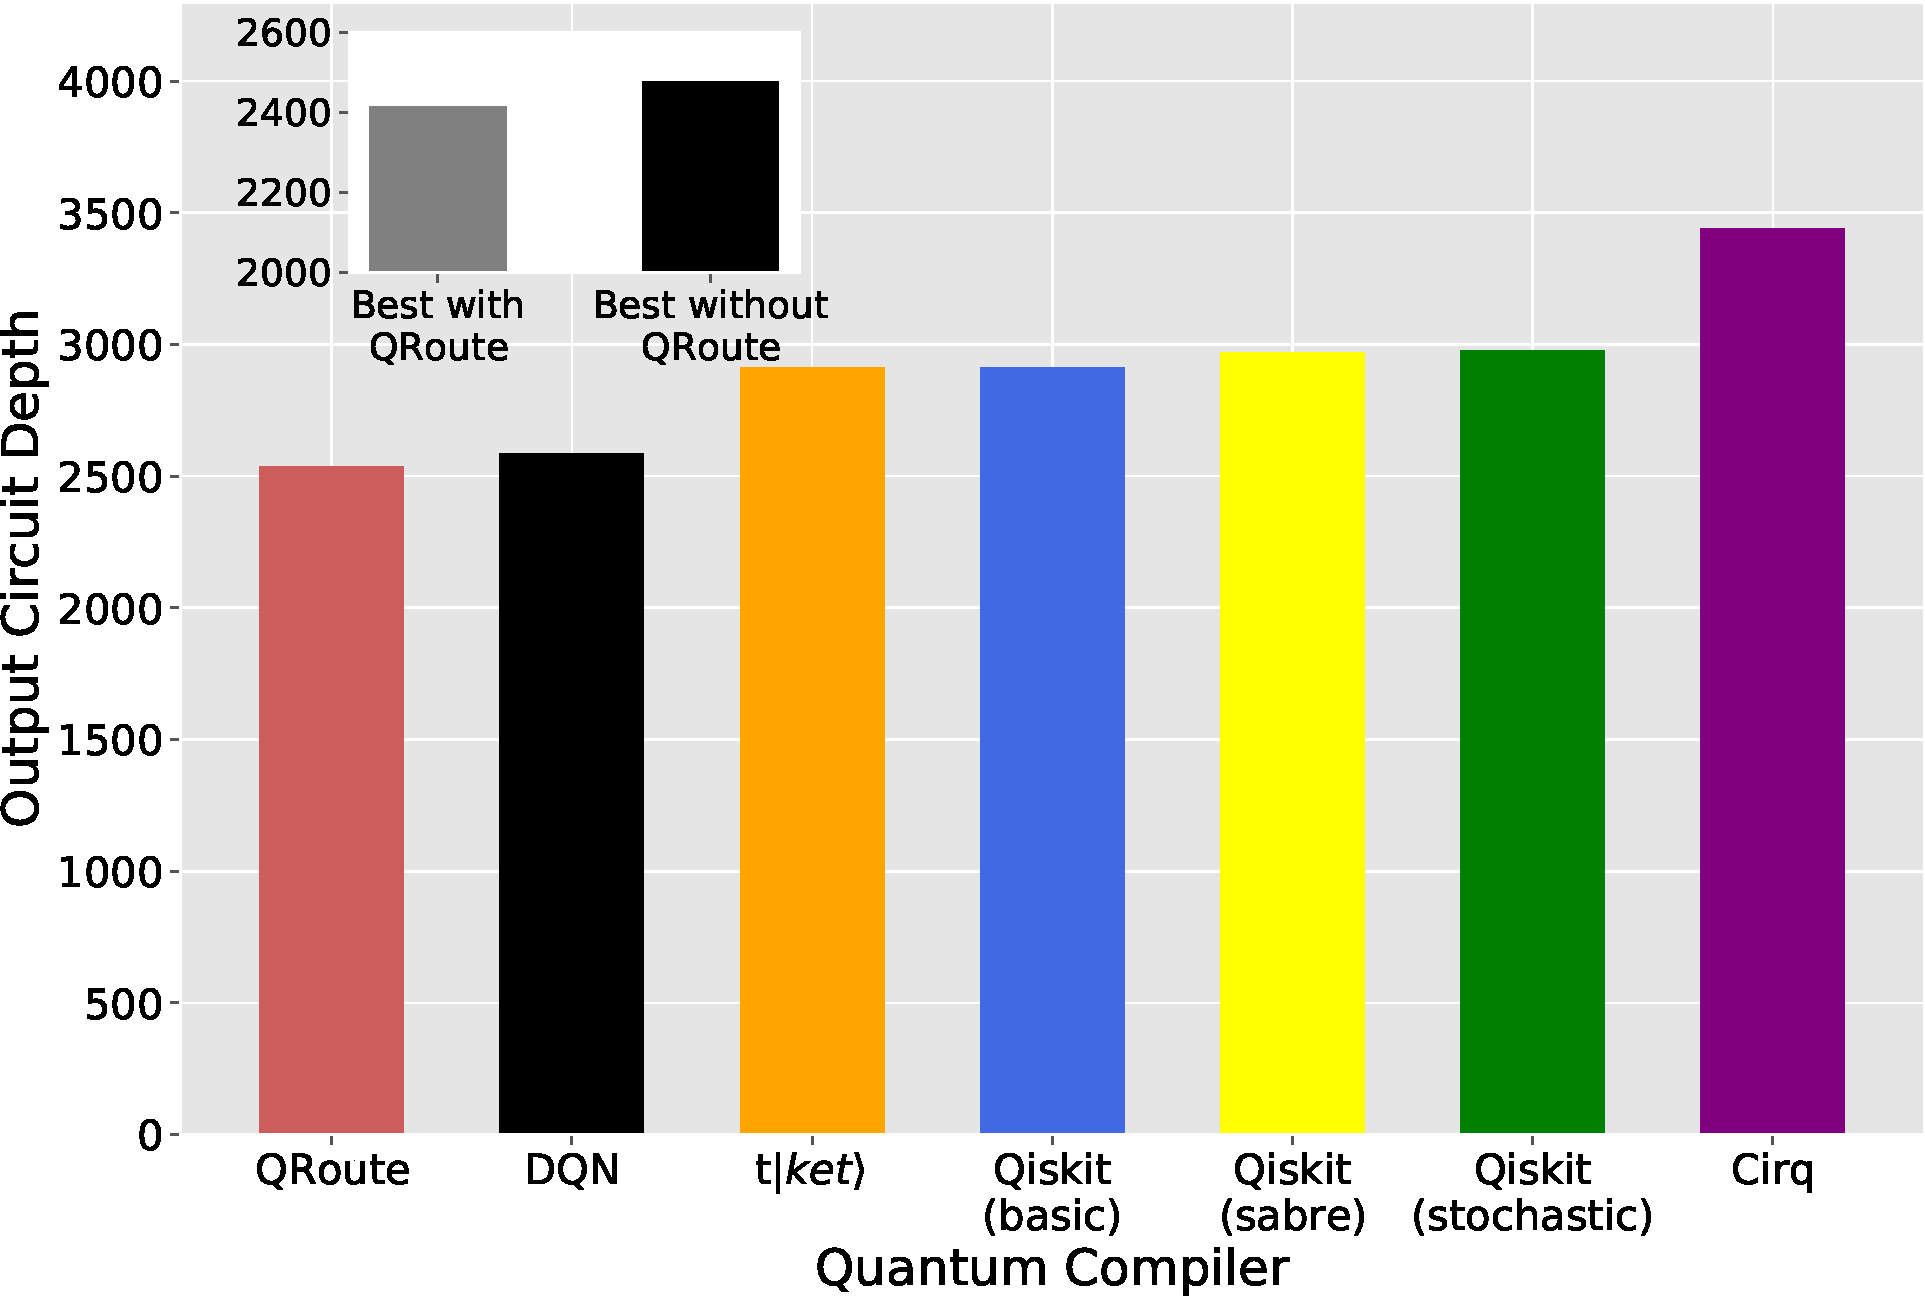
\includegraphics[width=\linewidth]{figures/qroute/realistic_small_benchmark.pdf}
    \caption[qRoute Results on small realistic circuit set]{\label{fig:results-small}
        Plots of output circuit depths of routing algorithms over small realistic circuits ($\leq 100$ gates), summed over the entire dataset. The inset shows the results on the same data comparing the best performant scheduler excluding and including QRoute on each circuit respectively.}
\end{figure}



\begin{figure*}[ht]
    \centering
    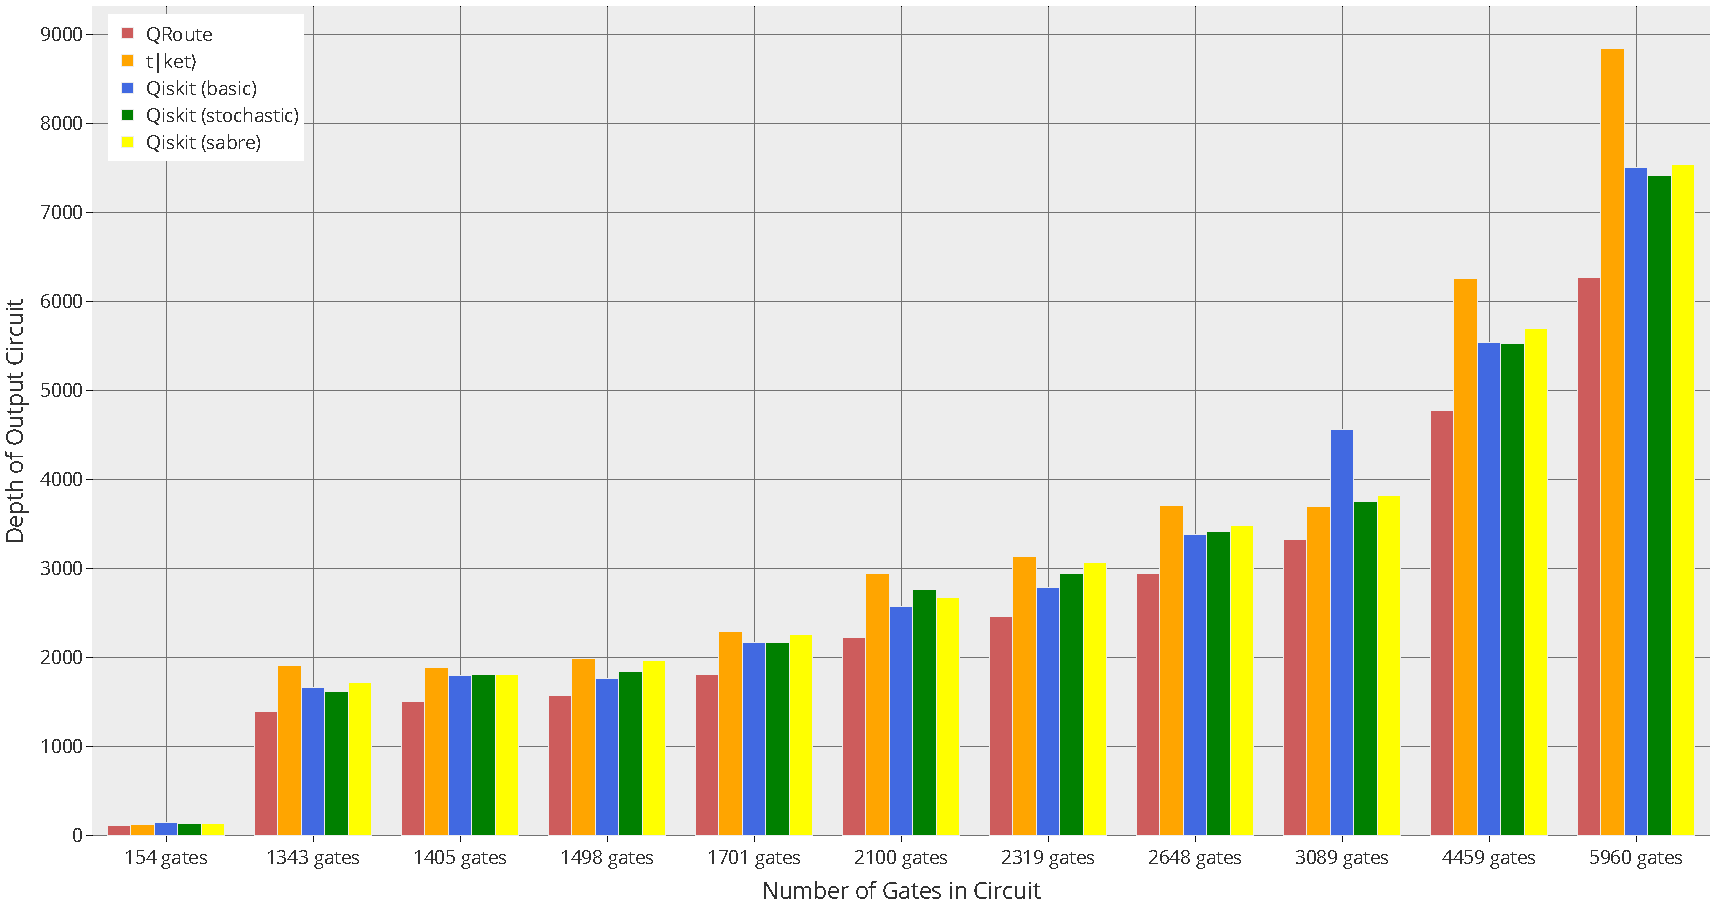
\includegraphics[width=\linewidth]{figures/qroute/realistic_large_benchmark.pdf}
    \caption[qRoute Results on large realistic circuit set]{\label{fig:results-large}
        The results over eight circuits sampled from the large realistic dataset benchmark, the outputs of each routing algorithm are shown for every circuit.}
\end{figure*}

On this dataset also, closest to QRoute performance is shown by Deep-Q-Network guided simulated annealer. To compare performances, we look at the average circuit depth ratio (CDR), which is defined by \cite{qroute_dqn2}:
\begin{equation}
    \text{CDR} = \frac{1}{\textrm{\#circuits}} \sum_{\textrm{circuits}} \frac{\textrm{Output Circuit Depth}}{\textrm{Input Circuit Depth}}
    \label{eq:CDR}
\end{equation}
The resultant CDR for QRoute is $1.178$, where as the reported CDR for the DQN is $1.19$. In fact, QRoute outperforms DQN on at least $80\%$ of the circuits. This is significant because in contrast to the random circuit benchmark, the realistic benchmarks consist of the circuits that are closer to the circuits used in useful computation.


\subsection{\label{sec:results-realistic}Large Realistic Circuit}

For final benchmark, we take eight large circuits ranging from 154 gates to 5960 gates in its input from the IBM-Quantum realistic test dataset \cite{data_realistic}. The results are plotted in Fig.  \ref{fig:results-large}. QRoute has the best performance of all available routing methods: Qiskit and t$\ket{\text{ket}}$, on every one of these sampled circuits with on an average $13.6\%$ lower circuit depth, and notable increase in winning difference on the larger circuits.



The results from DQN and Cirq are not available for these benchmarks as they are not designed to scale to such huge circuits. In case of DQN, the CDR data results were not provided for the circuits over $200$ gates, mainly because simulated annealing used in it is computationally expensive. Similarly, for Cirq, it takes several days to compile each of the near $5000$ qubit circuits. In contrast, QRoute is able to compile these circuits in at most 4 hours, and its compilation process can be sped up by reducing the depth of the search. Spending more time, however, helps MCTS to better approximate the Q-values leading to circuits with lower resulting depth.



\section{\label{sec:discussion-conclusion}Discussion and Conclusion}
%I'm writing this vaguely. Improve upon stuff wherever possible and let's meet at night. 

In this chapter, we have shown that the problem of qubit routing has a very powerful and elegant formulation in Reinforcement Learning (RL) which can surpass the results of any classical heuristic algorithm across all sizes of circuits and types of architectures. Furthermore, the central idea of building up solutions step-by-step when searching in combinatorial action spaces and enforcing constraints using mutex locks, can be adapted for several other combinatorial optimization problems \cite{comb_survey, comb_1, comb_2, comb_3, comb_4}. Our approach is flexible enough to compile circuits of any size onto any device, from small ones like IBMQX20 with 20 qubits, to much larger hardware like Google Sycamore (results provided in supplementary) with 53 qubits (the Circuit Depth Ratio for small realistic circuits on Google Sycamore was 1.64). Also, it intrinsically deals with hardware having different primitive instruction set, for example on hardware where SWAP gates are not a primitive and they get decomposed to 3 operations. QRoute enjoys significant tunability; hyperparameters can be changed easily to alter the tradeoff between time taken and optimality of decisions, exploration and exploitation, etc.

QRoute is a reasonably fast method, taking well under 10 minutes to route a circuit with under 100 operations, and at most 4 hours for those with upto 5000 operations, when tested on a personal machine with an i3 processor (3.7 GHz) and no GPU acceleration. Yet more can be desired in terms of speed. However, it is hard to achieve any significant improvement without reducing the number of search iterations and trading off a bit of performance. More predictive neural networks can help squeeze in better speeds.

One of the challenges of methods like DQN, that use Simulated Annealing to build up their actions is that the algorithm cannot plan for the gates which are not yet waiting to be scheduled, those which will come to the head of the list once the gates which are currently waiting are executed \cite{qroute_dqn2}. QRoute also shares this deficiency, but the effect of this issue is mitigated by the explicit tree search which takes into account the rewards that will be accrued in the longer-term future. There is scope to further improve this by feeding the entire list of future targets directly into our neural network by using transformer encoders to handle the arbitrary length sequence data. This and other aspects of neural network design will be a primary facet of future explorations. Another means of improving the performance  would be to introduce new actions by incorporating use of BRIDGE gates \cite{bridge_gate} and gate commutation rules \cite{utk_equiv_circuits} alongside currently used SWAP gates. The advantage of former is that it allows running CNOT gates on non-adjacent qubit without permuting the ordering of the logical qubits; whereas, the latter would allow MCTS to recognize the redundancy in action space, making its exploration and selection more efficient.

Finally, we provide an open-sourced access to our software library. It will allow researchers and developers to implement variants of our methods with minimal effort. We hope that this will aid future research in quantum circuit transformations. For review we are providing, the codebase and a multimedia in the supplementary.  

On the whole, the Monte Carlo Tree Search for building up solutions in combinatorial action spaces has exceeded the current state of art methods that perform qubit routing. Despite its success, we note that QRoute is a primitive implementation of our ideas, and there is great scope of improvement in future. 


%--------------------------------------------------------

\chapter{qLEET: Visualizing Loss Landscapes, Expressibility, Entangling power and Training Trajectories for Parameterized Quantum Circuits}
\label{ch:qleet}
\section{\label{qleet-sec:abstract}Abstract}

We present qLEET, an open-source Python package for studying parameterized quantum circuits (PQCs), which are widely used in various variational quantum algorithms (VQAs) and quantum machine learning (QML) algorithms. qLEET enables computation of properties such as expressibility and entangling power of a PQC by studying its entanglement spectrum and the distribution of parameterized states produced by it. Furthermore, it allows users to visualize the training trajectories of PQCs along with high-dimensional loss landscapes generated by them for different objective functions. It supports quantum circuits and noise models built using popular quantum computing libraries such as Qiskit, Cirq, and Pyquil. In our work, we demonstrate how qLEET provides opportunities to design and improve hybrid quantum-classical algorithms by utilizing intuitive insights from the ansatz capability and structure of the loss landscape.

{\smaller (Whitepaper on Arxiv, quant-ph, May 2022 \cite{self-qleet})}    

\section{\label{qleet-sec:intro}Introduction}

Recent advances in the field of quantum technologies have led to the development of near-term quantum hardware, more popularly referred to as noisy intermediate-scale quantum (NISQ) devices \cite{nisq_preskill, RevModPhys.94.015004}. Unfortunately, due to restrictive qubit connectivity, imperfect qubit control, and minimal error correction, their computation capabilities are limited to executing only low depth algorithms \cite{9251243}. For this reason, these devices are supposedly used as accelerators for their classical counterparts instead of stand-alone devices themselves. This has led to the development of hybrid quantum-classical (HQC) algorithms, which use both quantum and classical hardware either iteratively or sequentially. The problems are decomposed into classically tractable and intractable parts in such a setup, where the latter is solved using the quantum processor \cite{Endo2021-zy}. 

Parameterized quantum circuits (PQCs) are one of the fundamental components of these algorithms \cite{Benedetti2019-gz}. They are responsible for evolving the qubits system to a state which is dependent on the series of parameters ($\vec{\theta}$) provided by a classical processor and the objective function from some initial state $\ket{\psi_0}$. The initial state of the qubit system here could either be ground state $\ket{0\ldots0}$, or some other particular state such as Hartree-Fock state $\ket{\psi}_{HF}$ as in the case of electronic structure problems. The PQC ($U(\vec{\theta})$) is also popularly referred to as \textit{ansatz} \cite{Benedetti2019-gz}. Their structure dramatically affects the performance of HQCs as they influence both the (i) convergence speed, i.e., the number of quantum-classical feedback iterations, and (ii) closeness of the final state ($\ket{\psi({\vec{\theta}})}$) to a state that optimally solves the problem ($\ket{\psi({\vec{\theta}^*})}$), i.e., the overlap or the fidelity ($\mathcal{F} = |\langle\psi({\vec{\theta})} | \psi({\vec{\theta}^*})\rangle|^{2}$) \cite{9781107002173} between the final state and the target state. 

Therefore, it becomes imperative to design optimal PQCs for a given problem. However, this is not straightforward because their design depends not only on the problem instances themselves but also on the quantum hardware that executes them. After all, some essential properties like depth of circuit post compilation depend on the hardware's topology and the supported native gates. Overall, there exist three main classes of ansätze: (i) problem-inspired ansatz, where the evolutions of generators derived from properties of the given system are used to construct the PQCs \cite{Romero2018-uc}, (ii) hardware-efficient ansatz, where a minimal set of quantum gates native to a given device are used to construct the PQCs \cite{Kandala2017-wn}, and (iii) adaptive ansatz, which is midway between the former two ansätze \cite{PRXQuantum.2.020310}. Using these three classes, one can develop numerous ansatz designs for any given problem. However, to finally choose one, we need to have insights from the problems and a concrete strategy to compare their performances.

\begin{figure*}[!th]
    \centering
    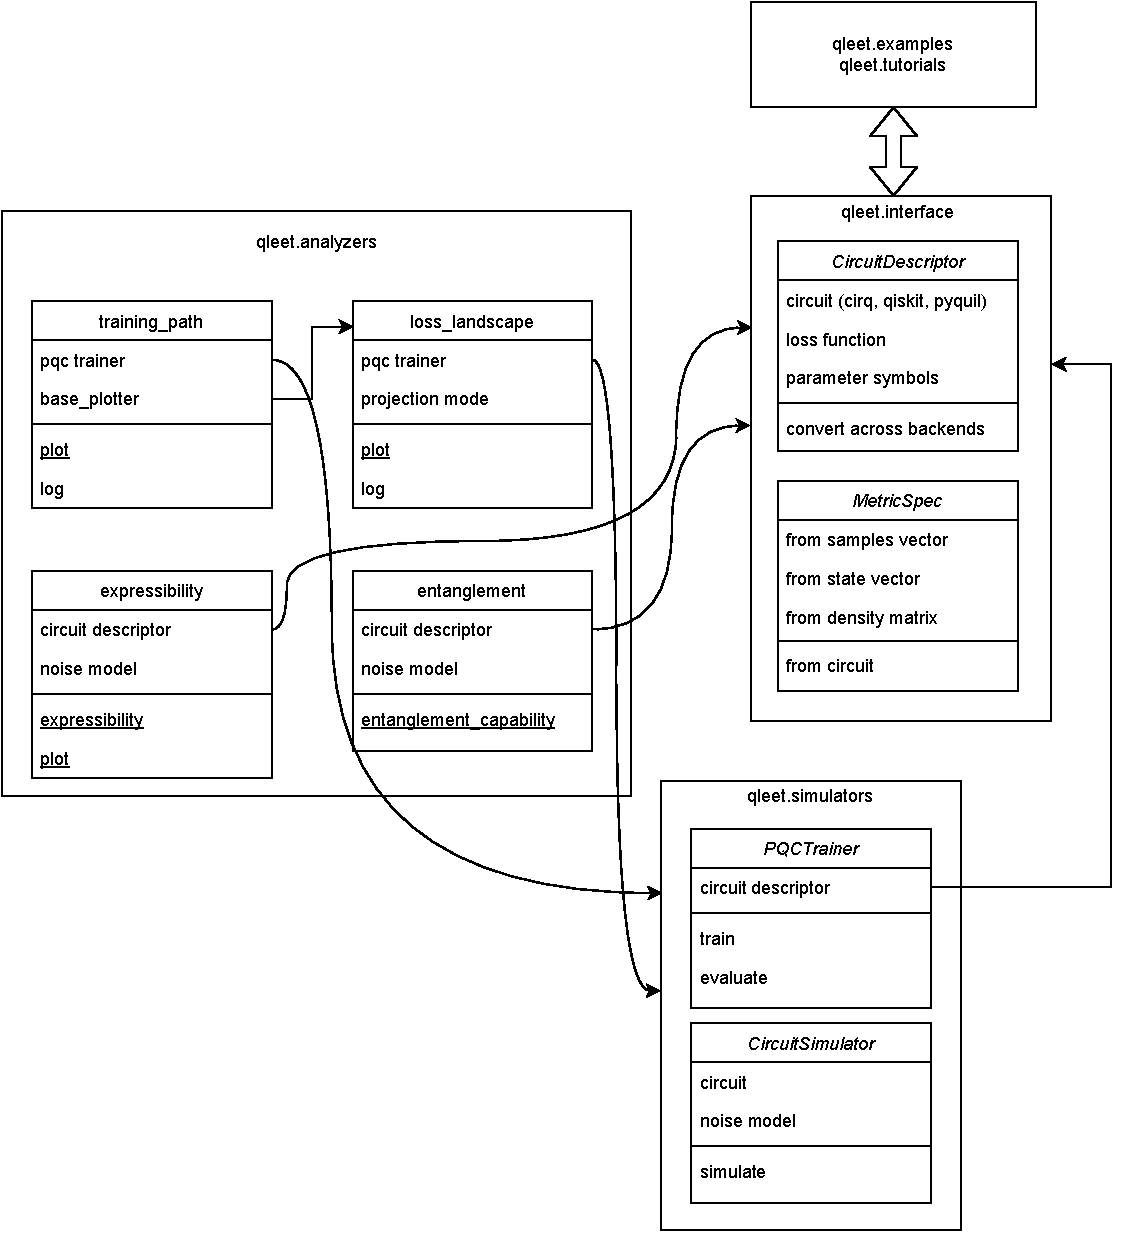
\includegraphics[width=0.65\linewidth]{figures/qleet/qleet-architecture.pdf}
    \caption[The architecture stack for qLEET]{The architecture stack for qLEET: Each block directed from qLEET represents a module. For the analyzers and simulators modules, each sub-block represents a submodule with class objects defined and used them (camel case) and function methods provided by them (underlined). For the interface module, each block represents the class objects defined in it (camel case header) and contains succinct description of their inputs and outputs.}
    \label{fig:qleet-architecture}
\end{figure*}

In this work, we present a python library called qLEET \footnote{\href{https://github.com/QLemma/qleet}{https://github.com/QLemma/qleet}}, \cite{qleet-zenodo}. The primary motivation behind the development of qLEET stems from this need to have a framework for analyzing the capabilities of parameterized quantum circuits and comparing their performances. It does so by allowing users to study various properties related to the behavior of PQCs and assess their effectiveness for a given problem instance. In particular, it will enable visualization of the loss landscape of a PQC for a given objective function and its training trajectory in the parameter space. Furthermore, it allows the calculation of some essential properties of PQCs, such as their expressibility and entangling power \cite{10.1002/qute.201900070}. It is integrable with other popular libraries such as Qiskit \cite{comp_qiskit}, Cirq \cite{comp_cirq}, or PyQuil \cite{ccquad_Pyquil} and also supports instruction-set languages like OpenQASM \cite{2021arXiv210414722C} and Quil \cite{ccquad_Pyquil}.

\textit{Structure} - In Sec. \ref{sec:overview} we present an overview of the architecture stack of qLEET. Then in Sec. \ref{sec:training} and Sec. \ref{sec:challenges}, we demonstrate the use of qLEET in the context of analyzing training of PQCs and mitigating the challenges associated with them. Finally, in Sec. \ref{sec:conclusion}, we conclude with a discussion about our current limitation and possible future extensions of this work.

\section{\label{sec:overview}Overview}

All the functionalities present in qLEET are grouped under four modules, which reside under the top-level module called \texttt{qleet}. Each such module provides modularity in feature development and interacts with one another via a specified workflow or API. We present the complete architecture stack for qLEET in Fig. \ref{fig:qleet-architecture}, listing down the following modules and identifying the interactions within them:

\begin{enumerate}

	\item \textbf{Interface module}: \texttt{qleet.interface} serves as the interface for users to build workflow of the variational computation by specifying the parameterized quantum circuit (PQC) along with its key components like symbolic placeholders for variational parameters ($\vec{\theta}$), an objective or a cost function ($\mathcal{C}$) as an observable in Pauli basis and some metrics for evolving the circuit to the final state defined by \texttt{MetricSpec}. It also contains \texttt{CircuitDescriptor}, which allows for the building of PQC using any supported framework, therefore making the computation software agnostic, and \texttt{MetaLogger}, which maintains the record for events that happen during qLEET's execution. 

	\item \textbf{Simulators module}: \texttt{qleet.simulator} contains the  simulation engine for performing the computation. Depending upon the type of workflow you want to execute, you can choose between \texttt{PQCTrainer} and \texttt{CircuitSimulator} for running training routing and for performing standalone circuit simulation, respectively. At this stage, you may also describe the simulation environment for the computation by providing a noise model for the system. 

	\item \textbf{Analyzers module}: \texttt{qleet.analyzers} performs execution of \texttt{CircuitDescriptor} object using \texttt{PQCTrainer} or \texttt{CircuitSimulator} functions present in the \texttt{qleet.simulator} module. Therefore, \texttt{qleet.analyzers} acts as a linkage between the previous two modules and is responsible for estimating various essential properties regarding PQC. These include loss landscape and training trajectory calculation or histogram prediction for variational computation and expressibility, entangling power and entanglement spectrum calculations for a given ansatz structure. This module also offers plotting functionality for some of these features.
	
	\item \textbf{Example module}: \texttt{qleet.examples} contains basic set of introductory tutorials and predefined templates for users to get started with using qLEET and contribute to it. These include examples of using \texttt{qleet.analyzers} for various kinds of calculations, as mentioned before.

\end{enumerate} 

We maintain the consistency of our codebase via unit testing, type checking, and format checker via pytest \cite{pytestx.y}, mypy \cite{mypy}, and black \cite{black}, respectively. Overall, we aim for the architecture stack for qLEET to follow object-oriented design principles, which helps us create a clean and modular software tool that is easy to test, debug, and maintain in the future. 

% \begin{figure*}[!tp]
%     \centering
%     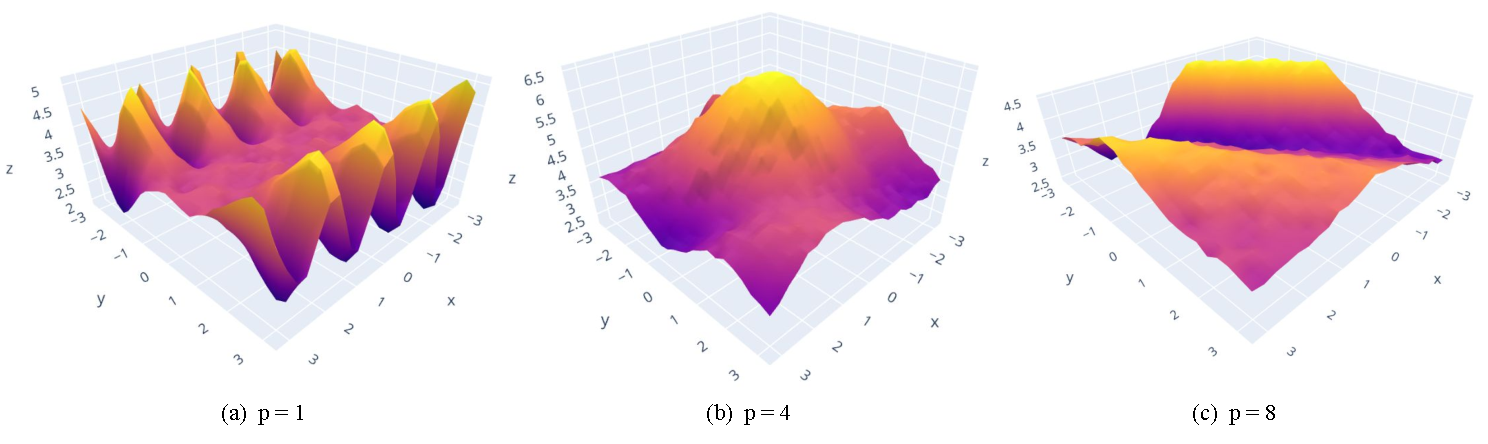
\includegraphics[width=\linewidth]{figures/qleet/loss-landscape.pdf}
%     \caption[Loss landscapes for QAOA]{Loss landscapes for solving Max-Cut problem for an Erdos-Renyi graph with $12$ nodes and $0.5$ edge probability, using QAOA for different values of $p$.}
%     \label{fig:qleet-loss}
% \end{figure*}


\section{\label{sec:features}Features}

This section presents the theory and examples for the features supported by the qLEET. We begin by introducing the idea of the trainability of a parameterized quantum circuit (PQC). From there, we would motivate the idea of studying different properties related to PQC to improve and analyze its trainability. We end the discussion in each subsection by demonstrating how modules in \texttt{qleet} can be used for analyzing the mentioned properties. 

\subsection{\label{sec:training}Trainability of PQCs}

We consider an N-qubit PQC $\hat{U}(\vec{\theta})$ with an objective function defined by a Hermitian observable $O$ in the Pauli basis. For an input quantum state $\rho$, the process of training is defined as minimizing the following function $\mathcal{C}$:
\begin{equation}
	\min \mathcal{C}(\vec{\theta}) = \min \text{Tr}[O \hat{U}(\vec{\theta}) \rho \hat{U}^{\dagger}(\vec{\theta})]
\end{equation}
A PQC $\hat{U}(\vec{\theta})$ evolves the input state $\rho$ to a parameterized target state $\rho(\vec{\theta})$ and to minimize $C(\vec{\theta})$ we update paramters $\vec{\theta}$ via some classical optimization routine such that:
\begin{equation}
	\vec{\theta}_{k+1} = \vec{\theta}_k - \gamma f(\nabla_{\vec{\theta}})\ \mathcal{C}, \quad f(\textbf{0})= 0 
\end{equation}
\begin{figure}[!tp]
    \centering
    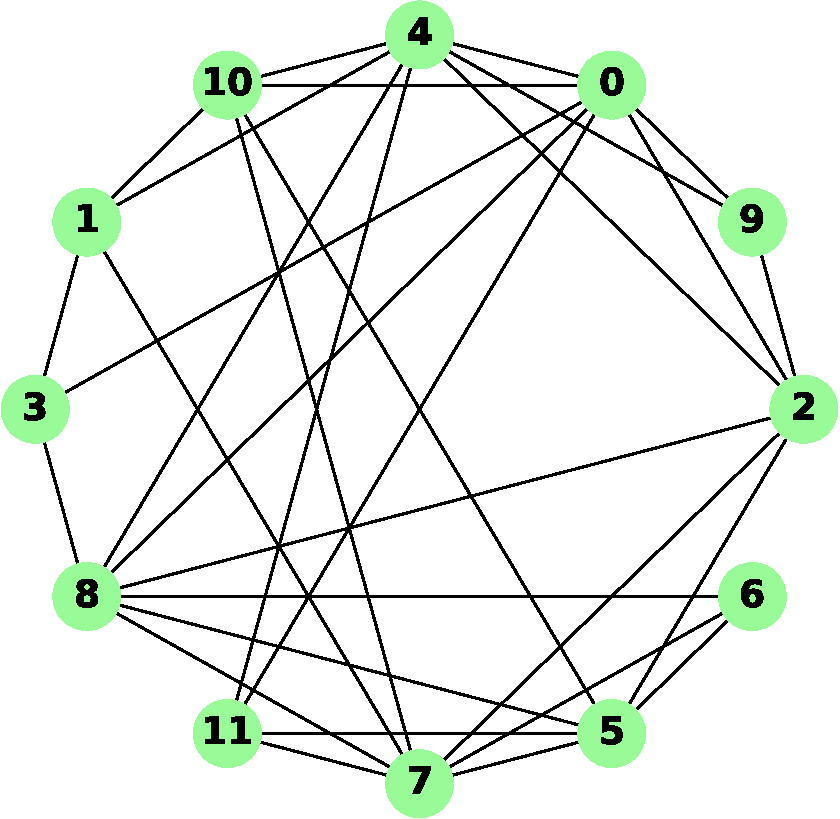
\includegraphics[width=0.6\linewidth]{figures/qleet/qaoa-graph.pdf}
    \caption[Problem graph for QAOA]{Problem graph considered for MaxCut using QAOA. It is generated as an Erdos-Renyi graph with $12$ nodes and $0.5$ edge probability.}
    \label{fig:qoao-maxcut-graph}
\end{figure}
Therefore, for successfully training a PQC, we would require contributions from any variational parameter $\theta_v$ to $\nabla_{\vec{\theta}}$, i.e., $\partial\mathcal{C}/\partial\theta_v$ to be non-vanishing, non-exploding and unbiased. This means that we expect $\mathbb{E}(\partial\mathcal{C}/\partial\theta_v) = 0$ and $\text{Var}(\partial\mathcal{C}/\partial\theta_v) > 0$  $\forall \theta_v \in \vec{\theta}$. However, this is not always the case, as we would see later in Sec. \ref{sec:challenges}. To better understand this behavior, it is critical to look at the evolution of $\mathcal{C}$ with respect to changes in variational parameters for which loss landscape and training path is beneficial. Furthermore, it has also been shown that circuits with $\nabla_{\vec{\theta}}\ \mathcal{C} \rightarrow 0$ for circuits with large expressibility. Hence, it is also crucial to not just look at the evolution of $\mathcal{C}$ but also get insights from the intrinsic properties of the PQC itself, such as its expressibility and entangling power.

\begin{figure*}[htp]
    \centering
    \begin{subfigure}[b]{0.32\linewidth}
        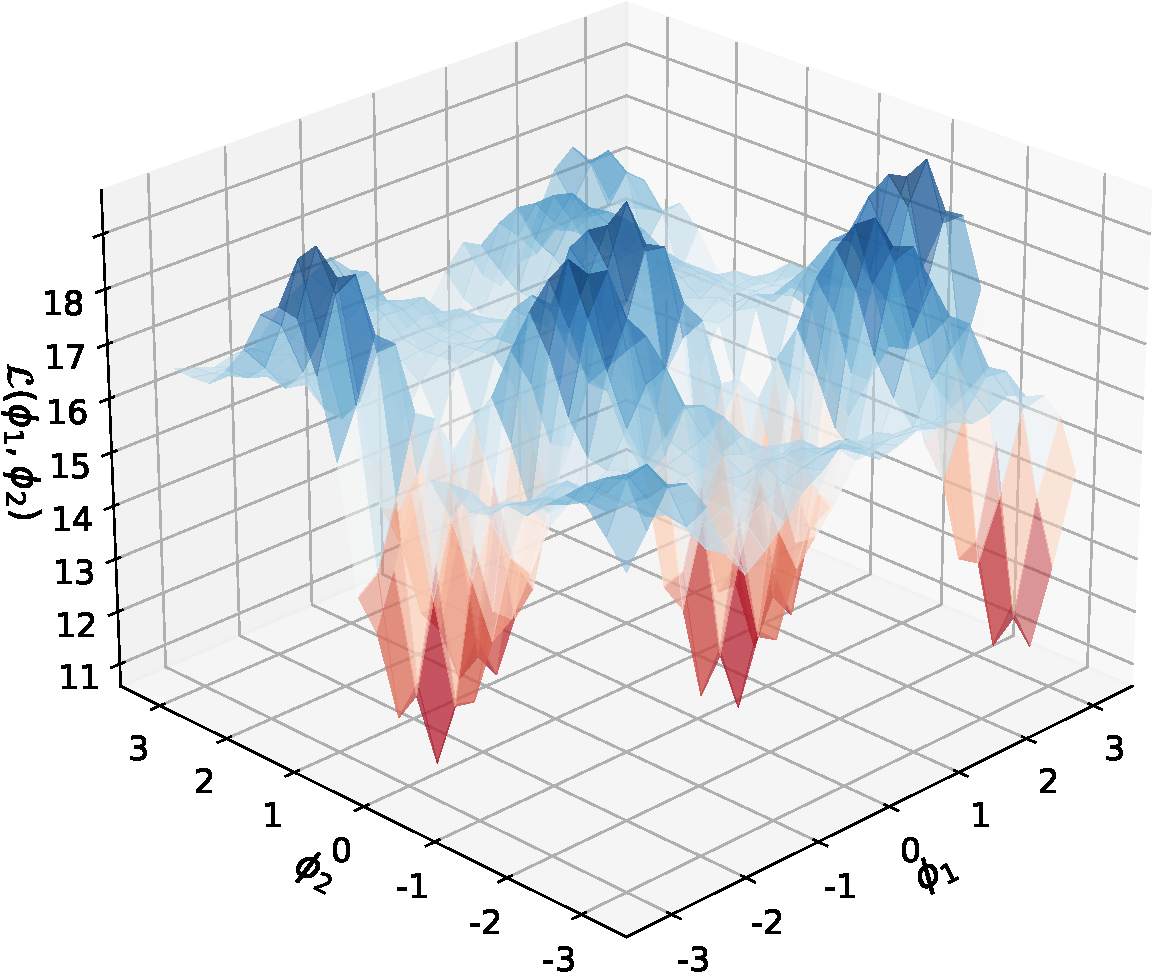
\includegraphics[width=\textwidth]{figures/qleet/loss_landscape_p1.pdf}
        \caption{Loss Landscape for $p=1$\label{fig:loss-p1}}
    \end{subfigure}
    \begin{subfigure}[b]{0.32\linewidth}
        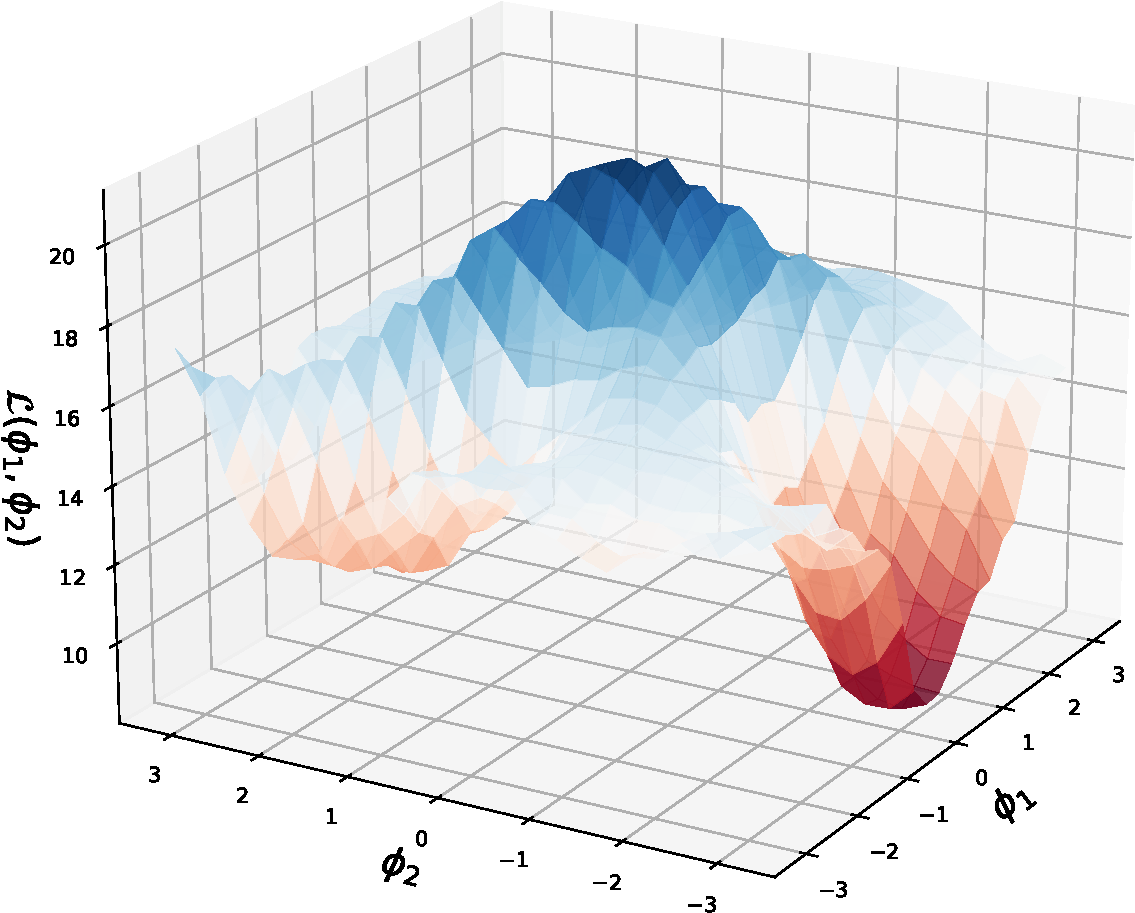
\includegraphics[width=\textwidth]{figures/qleet/loss_landscape_p2.pdf}
        \caption{Loss Landscape for $p=4$\label{fig:loss-p4}}
    \end{subfigure}
    \begin{subfigure}[b]{0.32\linewidth}
        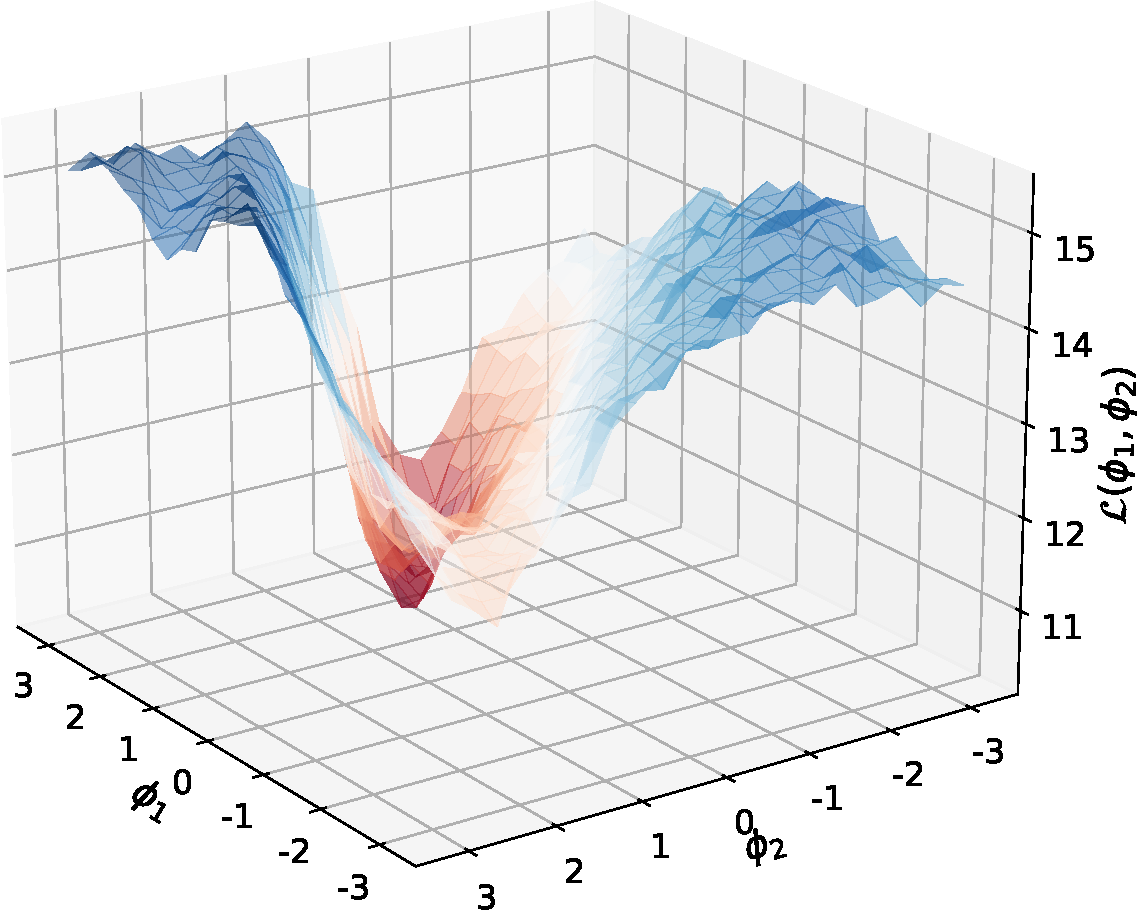
\includegraphics[width=\textwidth]{figures/qleet/loss_landscape_p3.pdf}
        \caption{Loss Landscape for $p=8$\label{fig:loss-p8}}
    \end{subfigure}%
    \hfill\newline
    \begin{subfigure}[b]{0.32\linewidth}
        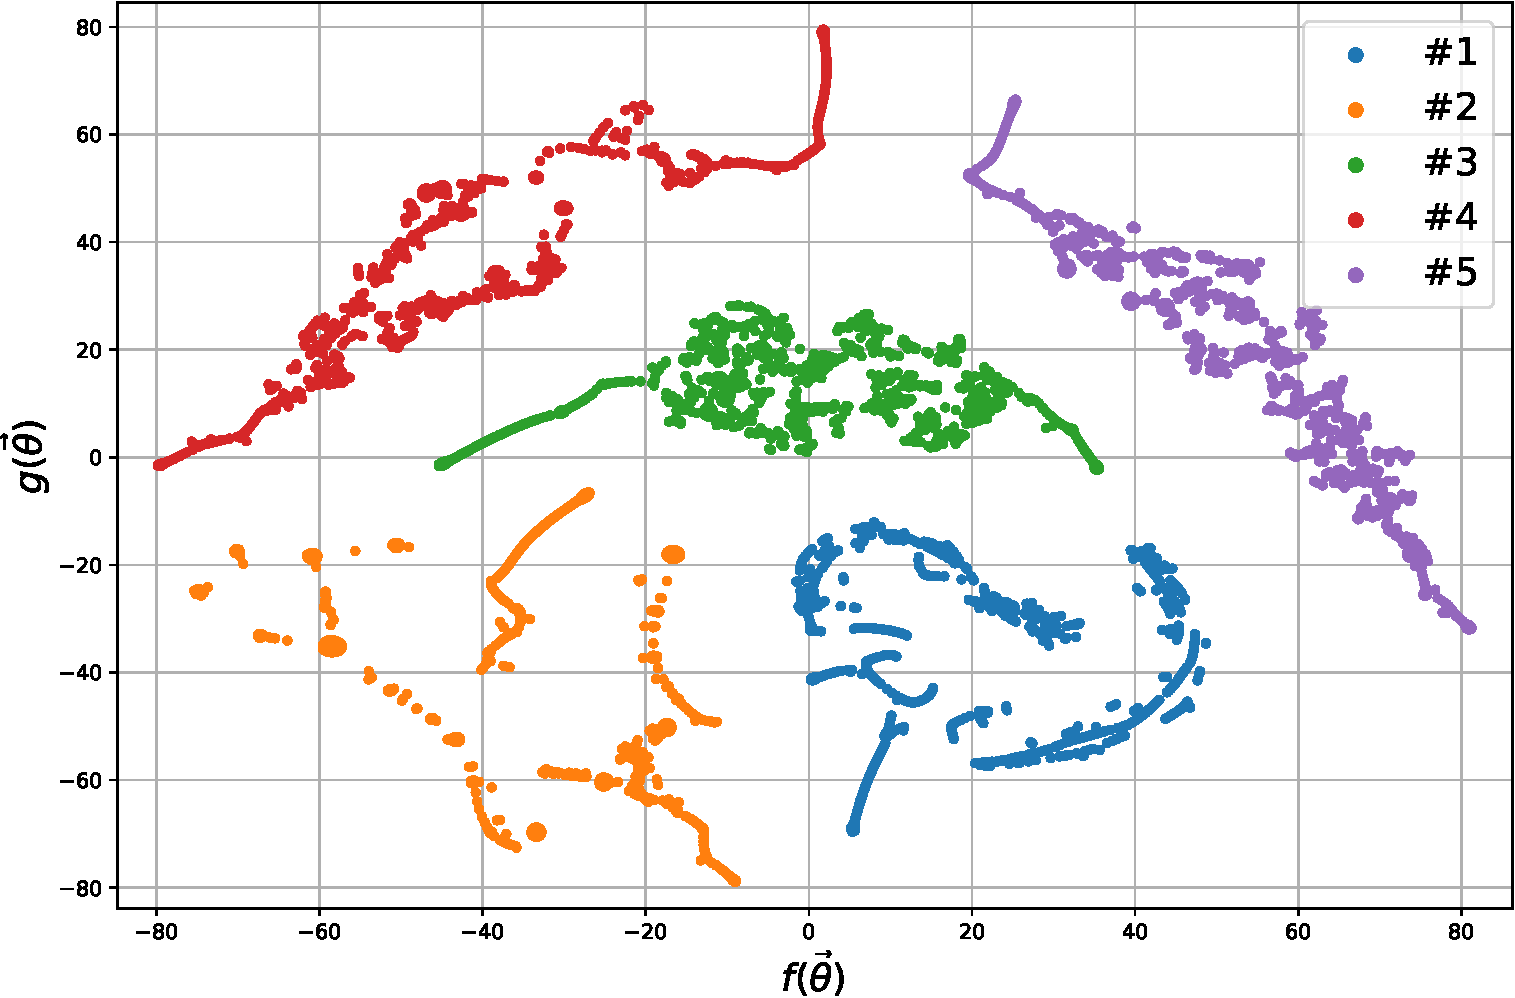
\includegraphics[width=\textwidth]{figures/qleet/training_trajectory_p1.pdf}
        \caption{Training trajectories for $p=1$\label{fig:train-p1}}
    \end{subfigure}
    \begin{subfigure}[b]{0.32\linewidth}
        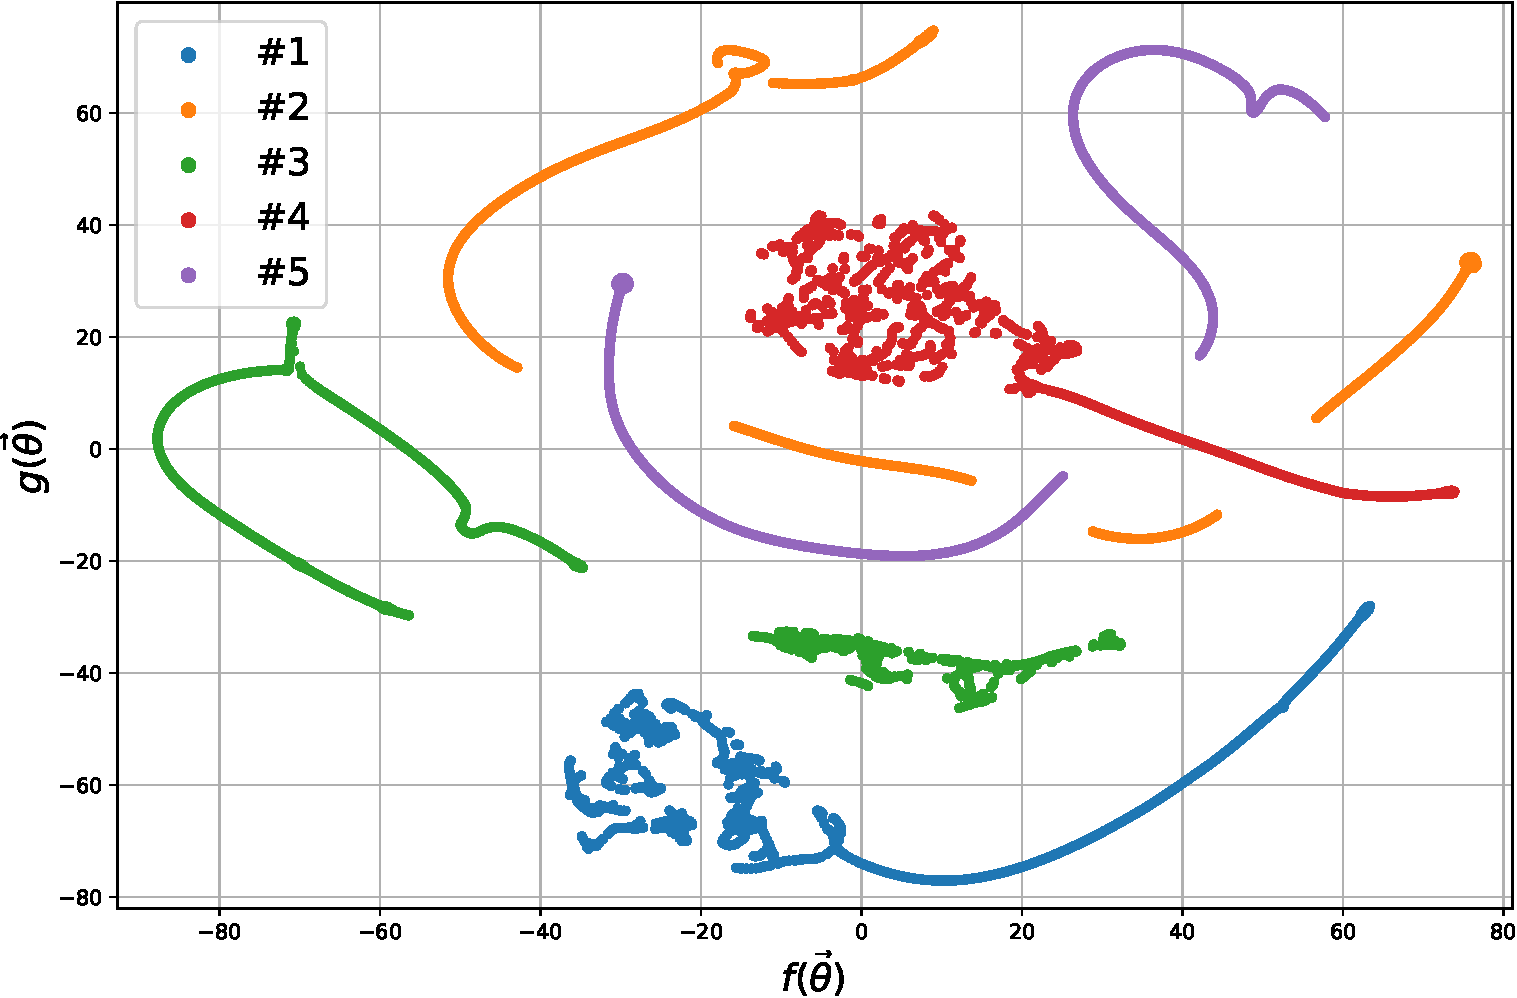
\includegraphics[width=\textwidth]{figures/qleet/training_trajectory_p2.pdf}
        \caption{Training trajectories for $p=4$\label{fig:train-p4}}
    \end{subfigure}
    \begin{subfigure}[b]{0.32\linewidth}
        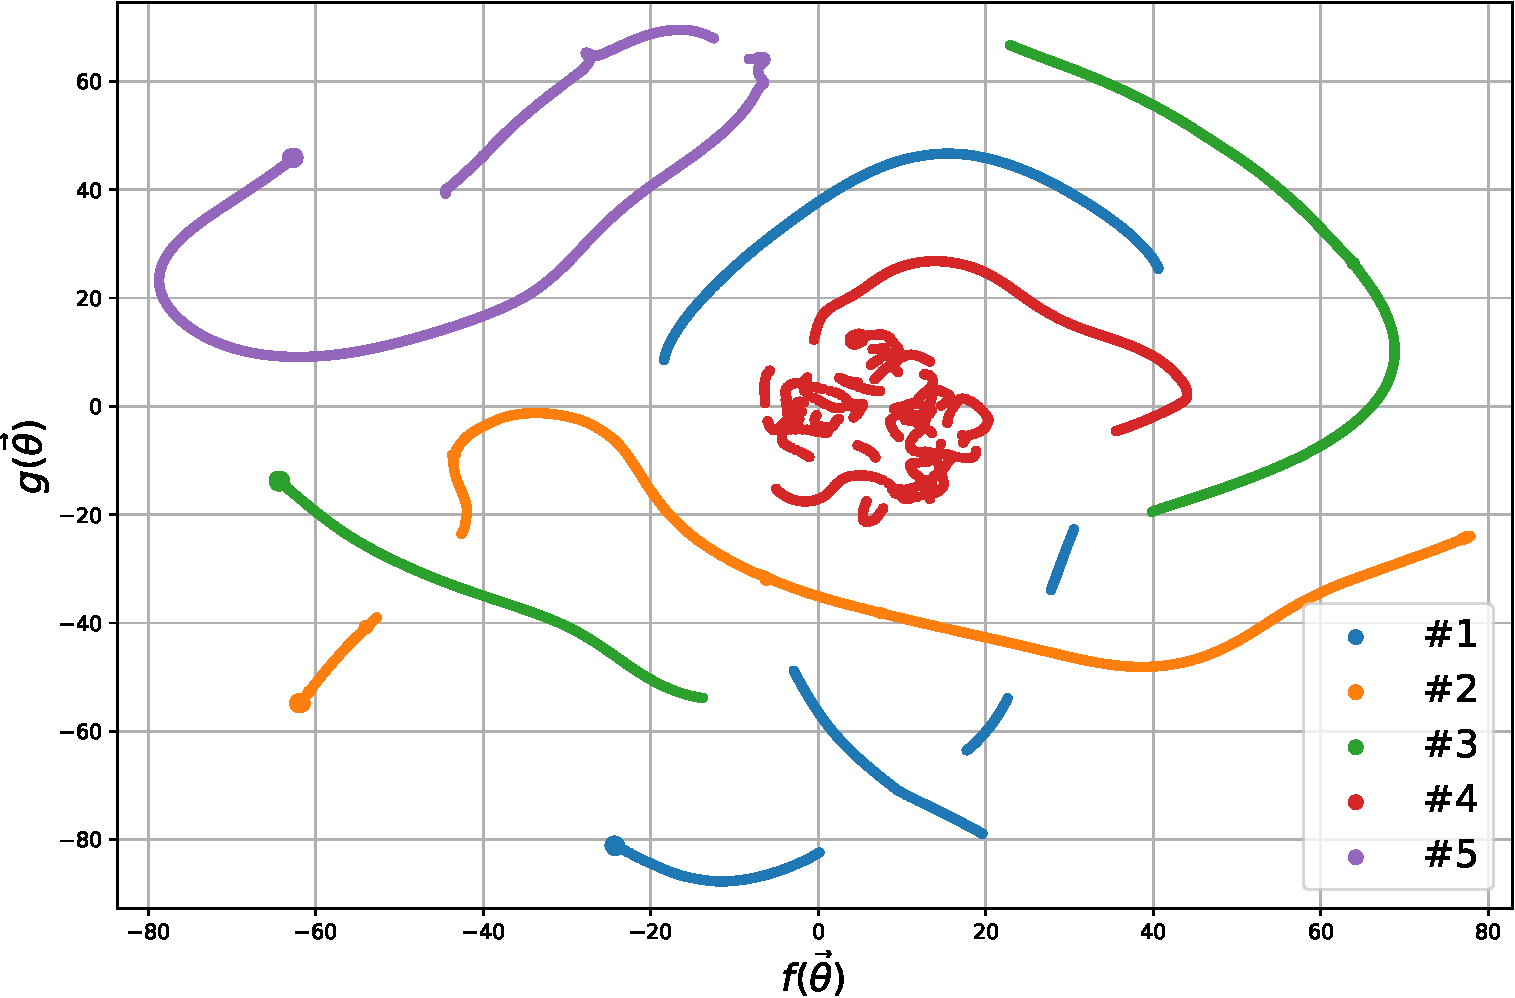
\includegraphics[width=\textwidth]{figures/qleet/training_trajectory_p3.pdf}
        \caption{Training trajectories for $p=8$\label{fig:train-p8}}
    \end{subfigure}%
    \caption[Loss Landscape and Training Trajectory for QAOA Max-Cut]{Loss landscape and training trajectories plots for solving the MaxCut problem using QAOA routine implemented with qLEET for the graph presented in Fig. \ref{fig:qoao-maxcut-graph}. The training trajectories have been plotted for five instances of training with different random initializations of variational parameters $\vec{\theta}$ for each value of $p\in\{1, 4, 8\}$, where $p$ denotes the number of times QAOA ansatz is repeated and functions $f(\vec{\theta})$ and $g(\vec{\theta})$ represented functions obtained after dimensionality reduction using t-SNE}
    \label{fig:loss-land-train-traj-qleet}
\end{figure*}

\subsection{Loss Landscape}

Loss landscape is a visual representation of the loss values or the $\mathcal{C}(\vec{\theta})$ around the trainable variational parameter space of the PQC. This inspection is usually done around the optimal variational parameters $\vec{\theta}^{*}$ to identify features like local minima, ridges, and valleys present in the loss surface. Such analysis helps in analyzing smoothness off the surface, indicating the ease with which a gradient-based optimizer might be able to perform on it \cite{loss-landscapes}. 

\begin{figure*}[!tp]
    \centering
    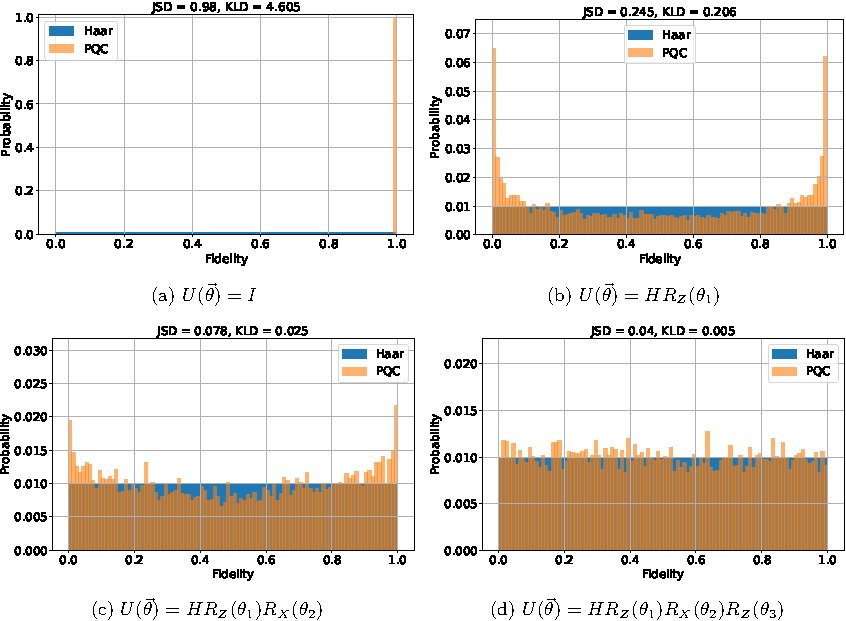
\includegraphics[width=0.82\textwidth]{figures/qleet/expressibility.pdf}
    \caption[Quantifying expressibility for single-qubit circuits]{Quantifying expressibility for single-qubit circuits. For each of the four circuits show here, 1000 sample pairs of circuit parameter vectors were uniformly drawn, corresponding to 2000 parameterized states. Histograms of estimated fidelities (orange) are shown, overlaid with fidelities of the Haar-distributed ensemble (blue), with the computed Kullback-Leibler (KL) divergence and Jensen-Shannon Distance (JSD) reported above the histograms.}
    \label{fig:expressibility}
\end{figure*}

For example, in Fig. \ref{fig:loss-land-train-traj-qleet}, we look at the loss landscape associated with solving the MaxCut problem using the QAOA algorithm \cite{2014arXiv1411.4028F} for an Erdos-Renyi graph (Fig. \ref{fig:qoao-maxcut-graph}). We see that as the number of layers of QAOA ansatz, parameterized by $p$, are increased, the loss landscape becomes much smoother, and local minima pits disappear. Therefore, it would be much easier for a descent-based optimizer to traverse to global minima in case of higher $p$. This and similar loss landscape calculations in qLEET are done using the \texttt{loss\_landscape} function present in the analyzer module. As shown in Eq. \ref{eqn:loss-landscape-plot}, we compute the value of the loss function $\mathcal{L}$ for all the parameters in an orthonormalized 2-D subspace $S$ with basis vectors $\phi_i$ sampled from the whole trainable variational parameter space. 
\begin{equation}\label{eqn:loss-landscape-plot}
    \begin{split}
        \mathcal{L}(\phi_i) 
        &= \mathcal{C}_{\text{PQC}}(\vec{\theta}^* + \vec{\phi_i}), \quad \vec{\phi_i} = \sum_i \alpha_i \theta_i\\ 
        &= \sum_{O} \text{Tr}\Bigg[O\rho \bigg(\vec{\theta}^* + \vec{\phi_i} \bigg) \Bigg]
    \end{split}
\end{equation}
We gather different information about the loss of landscape based on how we choose to perform the sampling. For example, using principal component analysis (PCA) over the set of variational parameters $\vec{\theta}$ at each training step would give us the vectors $\vec{\phi}$ that represent the directions in parameter space for which major changes happen during that training step. Similarly, other methods for obtaining subspace could be used, such as doing random sampling of basis vectors or t-SNE (t-Distributed Stochastic Neighbor Embedding) of the parameter vectors encountered in the training trajectory. All such methods provide beneficial insights about the structure of the loss landscape using which one could adapt their training strategy by tweaking the optimization routine, evaluation metric, etc. 

\subsection{Training Trajectory}

In many cases, just looking at the loss landscape for a given PQC model is not enough as we define the subspace $S$ using two of many possible directions as axes by taking linear combinations of variational parameters, while the loss landscape itself is highly nonlinear. Moreover, the high dimensionality of the parameter space makes the task of visualization of loss landscape extremely challenging. However, both of these difficulties can somewhat be alleviated by visualizing the loss landscape via the evolution of variational parameters of PQC during training in low dimensions. This evolution of variational parameters can be realized as the training trajectory for the PQC, and plotting them over several re-initializations helps us learn about the convergence properties of the PQCs and their optimization schedules. 

In qLEET, training trajectories are calculated inside the analyzer module by the \texttt{training\_path} function. We use the entire set of variational parameters $\vec{\theta}^{t}$ to generate the trajectory over all re-initialization for every time step $t$ in the training process. We project the parameter vectors down to an orthonormalized 2-D subspace $S$ using techniques such as PCA \cite{Jolliffe2016}, t-SNE \cite{NIPS2002_6150ccc6}, or PHATE \cite{Moon2019}. Similar to the case of loss landscape visualization, each of the mentioned techniques reveals different trajectory characteristics depending on its ability to preserve both global and local structures of higher-dimensional data in low dimensional subspace. Furthermore, the 2-D projections of the parameter trajectories can also be plotted on the loss surface, with the loss values as its third axis \cite{training-trajectories}.

For example, we present the training trajectories with t-SNE projection in Fig. \ref{fig:loss-land-train-traj-qleet} for the same MaxCut problem that we discuss in the previous subsection about the loss landscape. We look at five different training instances for each $p$, where we begin with randomized initialization of variational parameters $\vec{\theta}$ every time. We see that for $p=1$ evolutions of $\vec{\theta}$ for every instance happen in their own respective clusters, suggesting the optimizer unsuccessfully gets stuck for different local minima every time. In contrast, for both $p=4$ and $p=8$, we see much lesser clusters formation and more intercrossing, hinting at certain parameters $\theta_k$ evolving to the same values while the optimizer reaches the global minima.

% \begin{figure}[!tp]
%     \centering
%     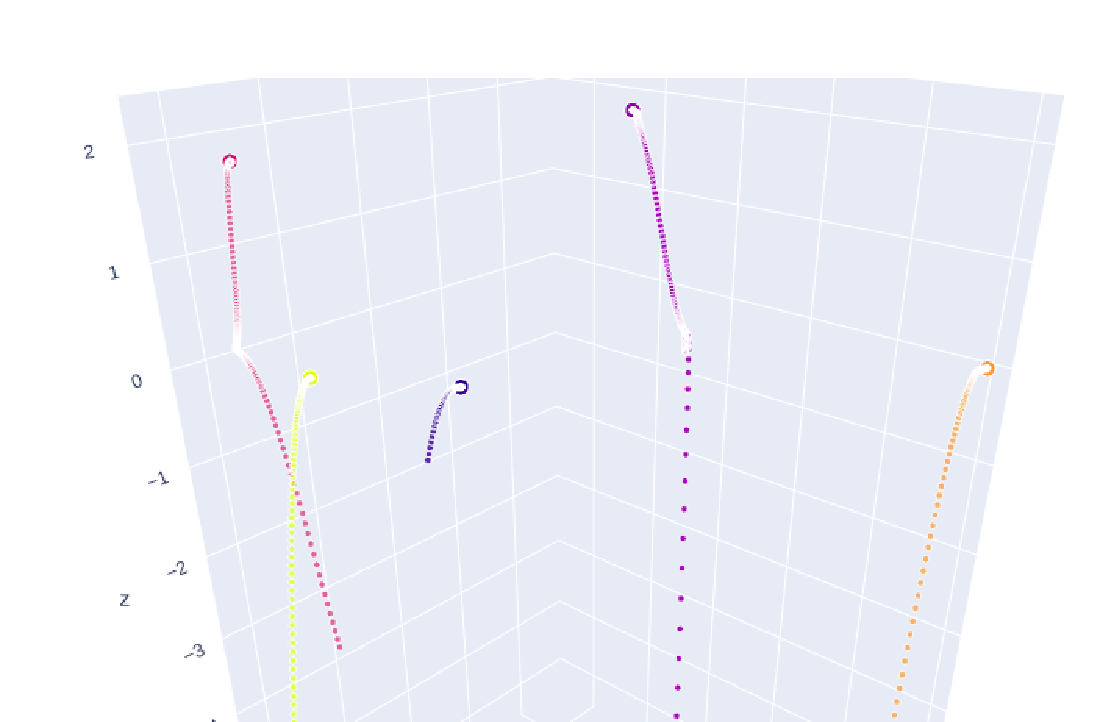
\includegraphics[width=\linewidth]{figures/qleet/training-trajectories.pdf}
%     \caption[Parameters in from several Training Trajectories]{This shows a 2-D projection of the parameter vectors plotted on the X-Y axes for 5 different re-initializations, each shown using a different color. These are collected over the entire optimization run and the final value of each run is plotted with a larger blob, visible at the top of each trajectory. The z-axis shows the loss value at that parameter vector. In this plot, it is visible that the trajectories do not mix and instead ascend up their own local optima, which indicates that sufficient exploration of the loss landscape was not performed and the optimization was very much local in nature and vary over different runs.}
%     \label{fig:expressibility}
% \end{figure}

\subsection{Expressibility}

We generate a distribution of states $\rho(\vec{\theta})$ for a PQC $\hat{U}(\vec{\theta})$ by randomly sampling over the variational parameter space. We quantify the deviation of this distribution from the one obtained from the maximally expressive Haar distribution as the \textit{Expressibility} of the given ansatz.
\begin{equation}\label{qleet:eq3}
    A^{(t)} =\left\Vert \int_\text{Haar}\rho^{\otimes t} \text{d}\rho - \int_{\vec{\theta}}\rho(\vec{\theta})^{\otimes t} \text{d}\rho(\vec{\theta}) \right\Vert_\text{HS}^2\,
\end{equation}
where $\int_\text{Haar}\text{d}\rho$ denotes the integration over the states $\rho$ distributed according to the Haar measure over the unitary group $\mathcal{U}$, $t$ represent the $t^{\text{th}}$ moment,  and $\left\Vert A \right\Vert_\text{HS}^2$ is the Hilbert-Schmidt norm calculated as $\text{Tr}(A^\dagger A)$. We compute Eq. \ref{qleet:eq3} as the divergence between the state fidelities $\mathcal{F}(\rho, \sigma) = \left(\text{Tr}\sqrt{\sqrt{\rho}\sigma\sqrt{\rho}} \right)^2$ \cite{Jozsa1994} generated from the ensemble of uniformly sampled parameterized states $\rho(\vec{\theta})$ to that of the ensemble obtained from uniform Haar distribution \cite{10.1002/qute.201900070}.
\begin{equation}
    \text{Expr} = D(\hat{P}_{PQC}(\mathcal{F}; \vec{\theta}) | P_{Haar}(\mathcal{F})), \quad \text{Expr} \geq 0
\end{equation}
According to this definition, a PQC $U(\vec{\theta})$ is more expressible if the distribution of state fidelities generated by the ansatz circuit $U(\vec{\theta})$ is closer to the one generated by the unitaries $U_{\text{Haar}}$ sampled uniformly from the unitary group $\mathcal{U}$. Therefore, the smaller the \textit{Expr} value, the more is the expressibility of the parameterized unitary. We see this in  Fig. \ref{fig:expressibility}, where we compare the fidelity distribution of PQC and Haar random states with respect to the number of Pauli rotation gates present in the single-qubit circuits and calculate the \textit{Expr} values for both Kullback-Leibler (KL) and Jensen-Shannon (JS) divergence. Furthermore, in Fig. \ref{fig:expressibility-measure}, we measure the increasing expressibility of the five qubit ansatz $U(\vec{\theta}) =  \prod_{1}^{L}\big(\bigotimes_{i=1}^{5}R_x(\theta_i^1)R_z(\theta_i^2)R_x(\theta_i^3) \ldots \bigotimes_{i<j}CX(i, j)\big)$, where we see how expressibility increases with the number of layers $L$.  Finally, we note that, in addition to experiments like these, \texttt{expressibility} function in qLEET can also be used to predict the likelihood of whether the given PQC would be able to represent an unknown N-qubit target state and do a comparative analysis between different ansätze.

\begin{figure}[!t]
    \centering
    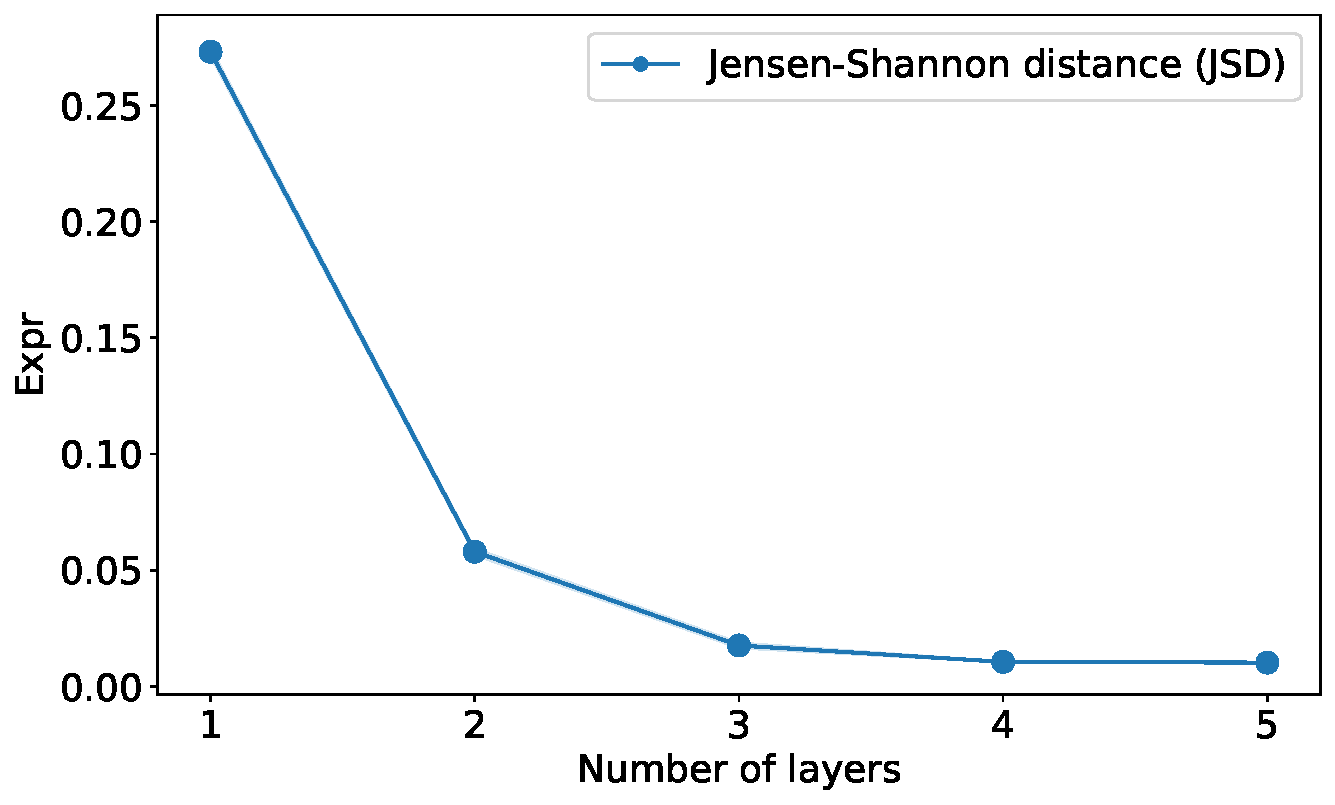
\includegraphics[width=\linewidth]{figures/qleet/expressibility-measure.pdf}
    \caption[Visualizing entanglement spectrum for parameterized quantum circuits]{Measuring expressibility for the parameterized quantum circuit $U(\vec{\theta}) =  \prod_{1}^{L}\big(\bigotimes_{i=1}^{5}R_x(\theta_i^1)R_z(\theta_i^2)R_x(\theta_i^3) \ldots \bigotimes_{i<j}CX(i, j)\big)$ using the Jensen-Shannon distance (JSD) measure as a function of number of layers $L$. }
    \label{fig:expressibility-measure}
\end{figure}

\begin{figure}[!t]
    \centering
    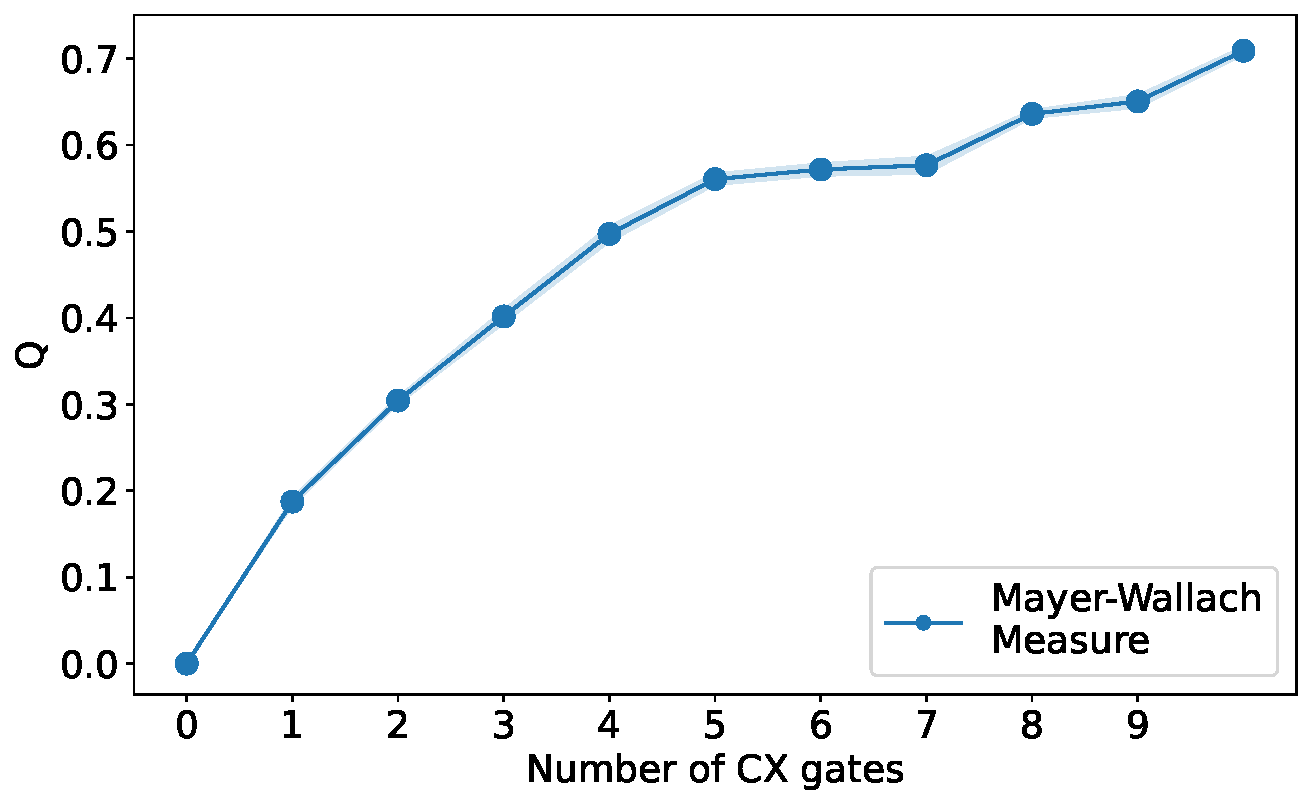
\includegraphics[width=\linewidth]{figures/qleet/entanglement-capability.pdf}
    \caption[Visualizing entanglement spectrum for parameterized quantum circuits]{Measuring entangling power for the parameterized quantum circuit $U(\theta)$ using the Mayer-Wallach measure as a function of the number of CX (or CNOT) gates appended to the circuit $U(\vec{\theta}) = \bigotimes_{i=1}^{5}R_x(\theta_i^1)R_z(\theta_i^2)R_x(\theta_i^3)$.}
    \label{fig:entanglement-capability}
\end{figure}

\subsection{Entangling Capability}

A fundamental property that makes quantum computation different from the classical one is the existence of entanglement in the system, which can be potentially exploited to gain a computational advantage. Hence, it is essential to quantify its ability to generate entanglement in the system to assess the effectiveness of a parameterized quantum circuit. We use entanglement measures to capture different properties of multipartite entanglement present in the system. The first measure that we use is the Meyer-Wallach $Q$ measure \cite{10.1002/qute.201900070, doi:10.1063/1.1497700} in which the amount of entangled states produced by a PQC is estimated by measuring the average entanglement between individual qubits and the rest of the system. In this context, the entangling capability of a PQC can be defined directly via the considered entanglement measure $Q$ averaged over all states $\rho(
\vec{\theta})$ generated by the PQC from the uniform sampling of variational parameters $\vec{\theta}$:

\begin{equation}
	Q = \frac{2}{|\vec{\theta}|}\sum_{\theta_{i}\in \vec{\theta}}\Bigg(1-\frac{1}{n}\sum_{k=1}^{n}\text{Tr}(\rho_{k}^{2}(\theta_{i}))\Bigg),
\end{equation}
where $\rho_k$ is the density matrix for the state of the $k$-th qubit. In a similar spirit, we can use another entanglement measure called Scott Measure \cite{10.1007/s11128-007-0052-7}, which generalizes the Meyer-Wallach measure using $m$ entanglement measures, each of which will measure the average entanglement between blocks of $m$ qubits and the rest of the system. Therefore, as pointed out before, each measure would give access to different properties related to multipartite entanglement, and as $m$ increases, $Q_m$ becomes more sensitive to correlations of an increasingly global nature. Similar to the previous case, the entangling capability of the PQC can be defined by the value of $Q_m$ measures, averaged over uniformly sampled $\vec{\theta}$ too:
\begin{equation}
    \begin{split}
        Q_{m} &= \frac{2^{m}}{(2^{m}-1) |\vec{\theta}|}\sum_{\theta_i \in \vec{\theta}} \bigg(1 - \\ 
        & \quad \quad \frac{m! (n-m)!)}{n!}\sum_{|S|=m} \text{Tr} (\rho_{S}^2 (\theta_i)) \bigg) \\
        m &= 1, \ldots, \lfloor n/2 \rfloor
    \end{split}
\end{equation}

In qLEET, we perform these calculations inside the $\texttt{entanglement}$ function in the analyzer module, where one can choose between both Meyer-Wallach and Scott measures for any PQC loaded as a $\texttt{CircuitDescriptor}$ object. For example, in Fig. \ref{fig:entanglement-capability}, we use it to plot the entangling capability of a five qubit circuit template $U(\vec{\theta}) = \bigotimes_{i=1}^{5}R_x(\theta_i^1)R_z(\theta_i^2)R_x(\theta_i^3)$ against the numbers of CNOT gates appended to circuit in a pair-wise fasion, i.e., CNOT$(i, j)$, where $i < j$ and $i,j <5$. We see that as the number of CNOT gates are increased, the entangling capability improves. We also notice a region of minimal increase between $[5, 7]$, which can be attributed to addition on qubits which were already transitive correlated.

\subsection{Entanglement Spectrum}

In the previous subsection, we quantified the entangling capability of an ansatz using entanglement measures. However, these measures might be insufficient to fully characterize all the properties related to multipartite entanglement \cite{PhysRevLett.115.267206}. This problem can be tackled by making use of the entanglement spectrum  \cite{PRXQuantum.1.020319}, which is defined as the eigenspectrum of the entanglement Hamiltonian $H_{\text{ent}}$:

\begin{equation}
    H_{\text{ent}} = -\log (\rho_A),
\end{equation}

where the $\rho_A = \text{Tr}_B(\rho)$ is the reduced density matrix of the qubit system obtained by the typical bipartition of the $N$ qubit system into subsystems $A$ and $B$ with $k = \lceil N/2 \rceil$ and $N-k$ qubits, respectively. For states sampled from maximally expressive Haar distribution, the eigenvalues $\xi_k$ of $H_{\text{ent}}$ follows the Marchenko-Pastur (MP) distribution \cite{10.1088/1751-8113/40/3/f04}. Therefore, we can quantify both expressibility and entangling power of the PQC by looking at the eigenspectrum of $H_{\text{ent}}^{\text{PQC}}$, calculated from uniformly sampled variational parameters $\vec{\theta}$. 

In qLEET, \texttt{entanglement\_spectrum} function in the analyzers module can be used for computing and plotting the entanglement spectrum for any given PQC $U(\vec{\theta})$. For example, in Fig. \ref{fig:entanglement-spectrum}, we use it to perform the entanglement spectrum analysis on a 16 qubit PQC, which is made of $L$ layers comprising three rotation gates on each qubit and CNOT gates between adjacent qubits, i.e., $U(\vec{\theta}) = \prod_{l}^{L}\big(\bigotimes_{i=0}^{15}R_x(\theta_i^1)R_z(\theta_i^2)R_x(\theta_i^3)\bigotimes_{i=0}^{14}CX(i, i+1)\big)$. We see that as the number of layers are increased in the ansatz, the eigenvalue distribution becomes more and more closer to the MP distribution. In fact, computing a divergence measure between these two distributions can also be used as a quantification of capability of the ansatz. 

\begin{figure}[!t]
    \centering
    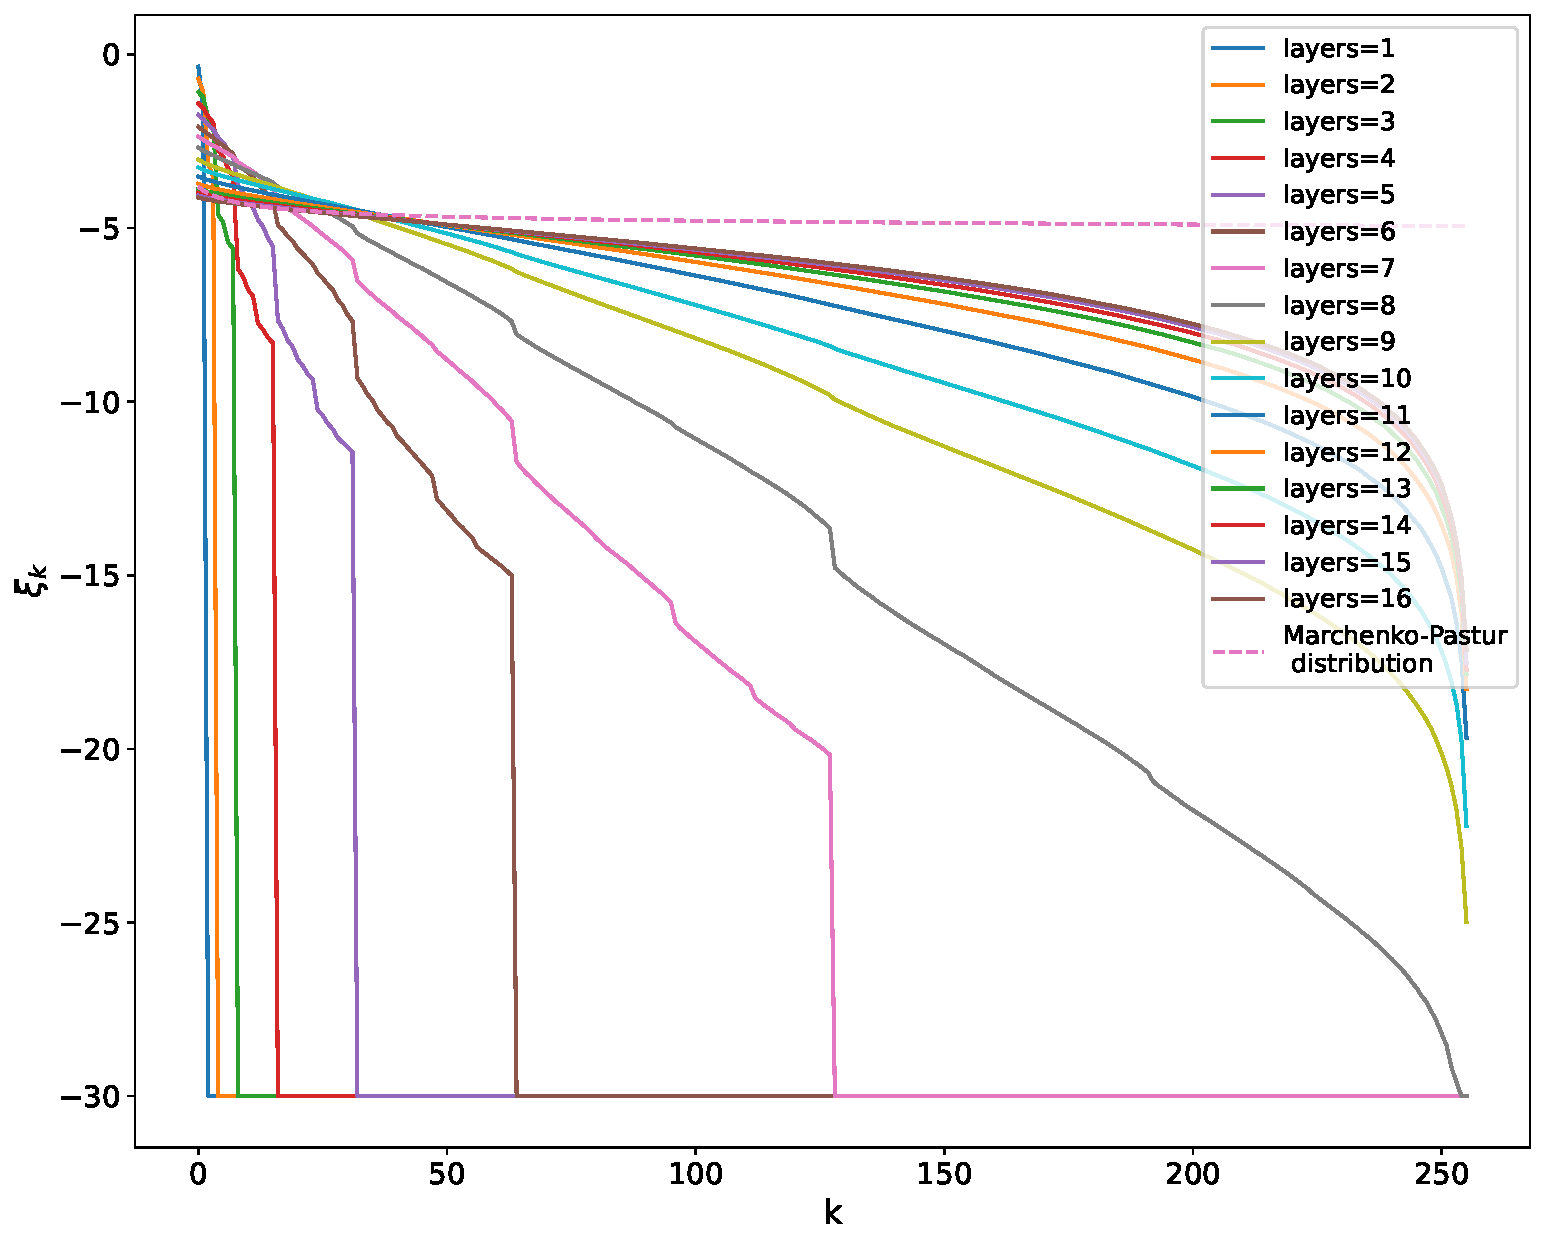
\includegraphics[width=\linewidth]{figures/qleet/entanglement-spectrum.pdf}
    \caption[Visualizing entanglement spectrum for parameterized quantum circuits]{Visualizing entanglement spectrum for a PQC $U(\vec{\theta}) = \prod_{1}^{L}\big(\bigotimes_{i=1}^{12}R_x(\theta_i^1)R_z(\theta_i^2)R_x(\theta_i^3) \ldots \bigotimes_{i=1}^{11}CX(i, i+1)\big)$. Here, $\xi_k$ are the eigenvalues of $H_{\text{ent}}^{U(\vec{\theta})}$ arranged in descending order and cut off at $-30$. The solid lines (blue to brown) represents the distribution $\xi_k$ for different layers $L$ and the dotted line (black) represents the ideal Marchenko-Pastur (MP) distribution. We see that as the number of layers is increased, the distribution of $\xi_k$ becomes more similar to MP distribution.}
    \label{fig:entanglement-spectrum}
\end{figure}


\begin{figure*}[t]
    \centering
    \begin{subfigure}[b]{0.48\textwidth}
    %\hspace{-20pt}
    \begin{minipage}
    {.03\textwidth}
        \caption{}
        \label{fig:barren-plateau-1}
    \end{minipage}%
    \begin{minipage}{0.90\textwidth}
        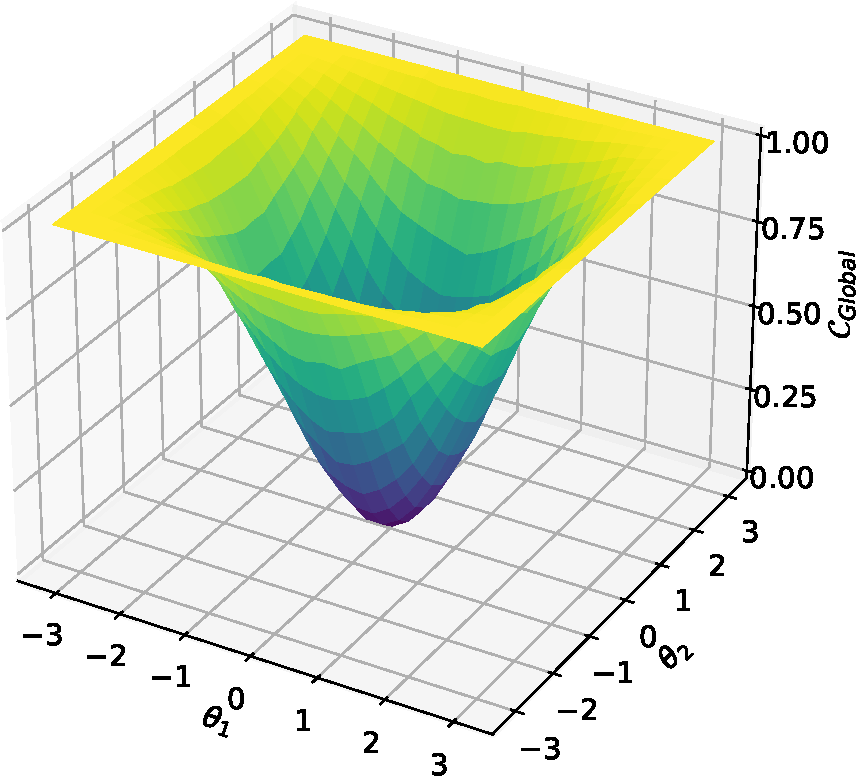
\includegraphics[width=.9\textwidth]{figures/qleet/global_cost_loss_landscape.pdf}
    \end{minipage}
    \end{subfigure}
    \begin{subfigure}[b]{0.48\linewidth}
    %\hspace{-35pt}
    \begin{minipage}{.08\textwidth}
        \caption{}
        \label{fig:barren-plateau-2}
    \end{minipage}%
    \begin{minipage}{0.9\textwidth}
        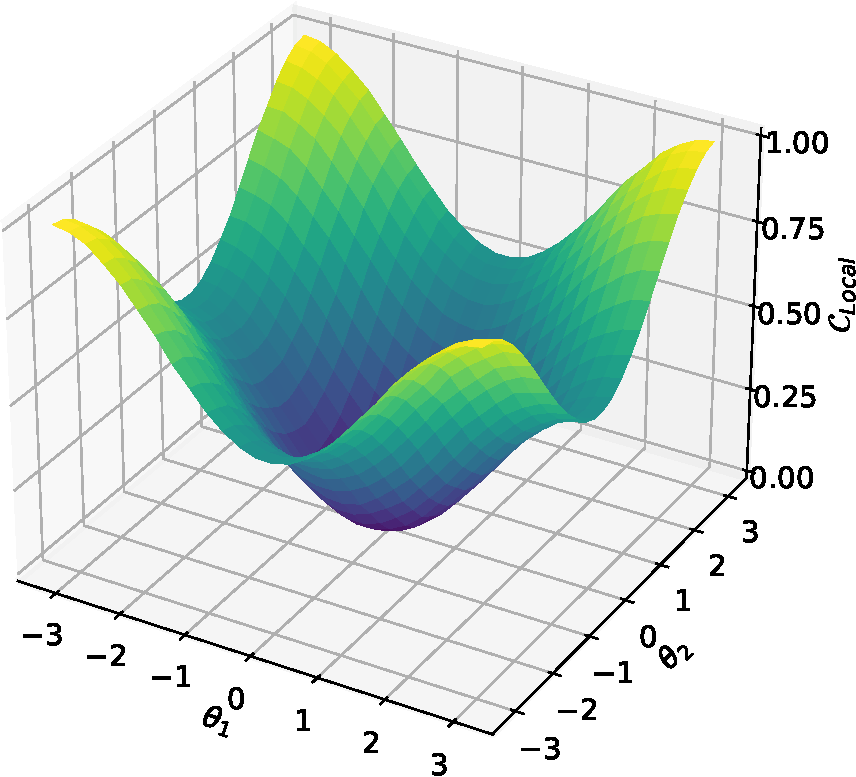
\includegraphics[width=0.9\textwidth]{figures/qleet/local_cost_loss_landscape.pdf}
    \end{minipage}
    \end{subfigure}\\
    \begin{subfigure}[b]{0.48\linewidth}
    %\hspace{-20pt}
    \begin{minipage}
    {.03\textwidth}
        \caption{}
        \label{fig:barren-plateau-3}
    \end{minipage}%
    \begin{minipage}{0.90\textwidth}
        \includegraphics[width=.9\linewidth]{figures/qleet/Global_cost_grad_landscape.pdf}
    \end{minipage}
    \end{subfigure}
    \begin{subfigure}[b]{0.48\textwidth}
    %\hspace{-35pt}
    \begin{minipage}{.08\textwidth}
        \caption{}
        \label{fig:barren-plateau-4}
    \end{minipage}%
    \begin{minipage}{0.9\textwidth}
        \includegraphics[width=0.9\textwidth]{figures/qleet/Local_cost_grad_landscape.pdf}
    \end{minipage}
    \end{subfigure}
    %\hspace{40pt}
    \caption[Presence of barren plateaus in parameterized quantum circuits]{Here we show the emergence of barren plateaus in the task of learning an Identity gate using the ansatz $R_X(0,\theta_1)R_X(1, \theta_2)CZ(0, 1)$ solely based on the choice of the cost function. Figures (a) and (b) represents the loss landscape for the $\mathcal{C}_{Global}$ and local $\mathcal{C}_{Local}$ cost functions, respectively. Similarly, figures (c) and (d) represents coloured heat maps for their  corresponding gradients $\nabla_{\theta_2}\mathcal{C}_{\text{Global}}$ and $\nabla_{\theta_2}\mathcal{C}_{\text{Local}}$} 
    %We see that for $\mathcal{C}_{Global}$, the gradients vanish rapidly towards the boundaries of the loss landscape.}
    \label{fig:barren-plateau}
\end{figure*}

% \begin{figure}[ht]
%     \centering
%     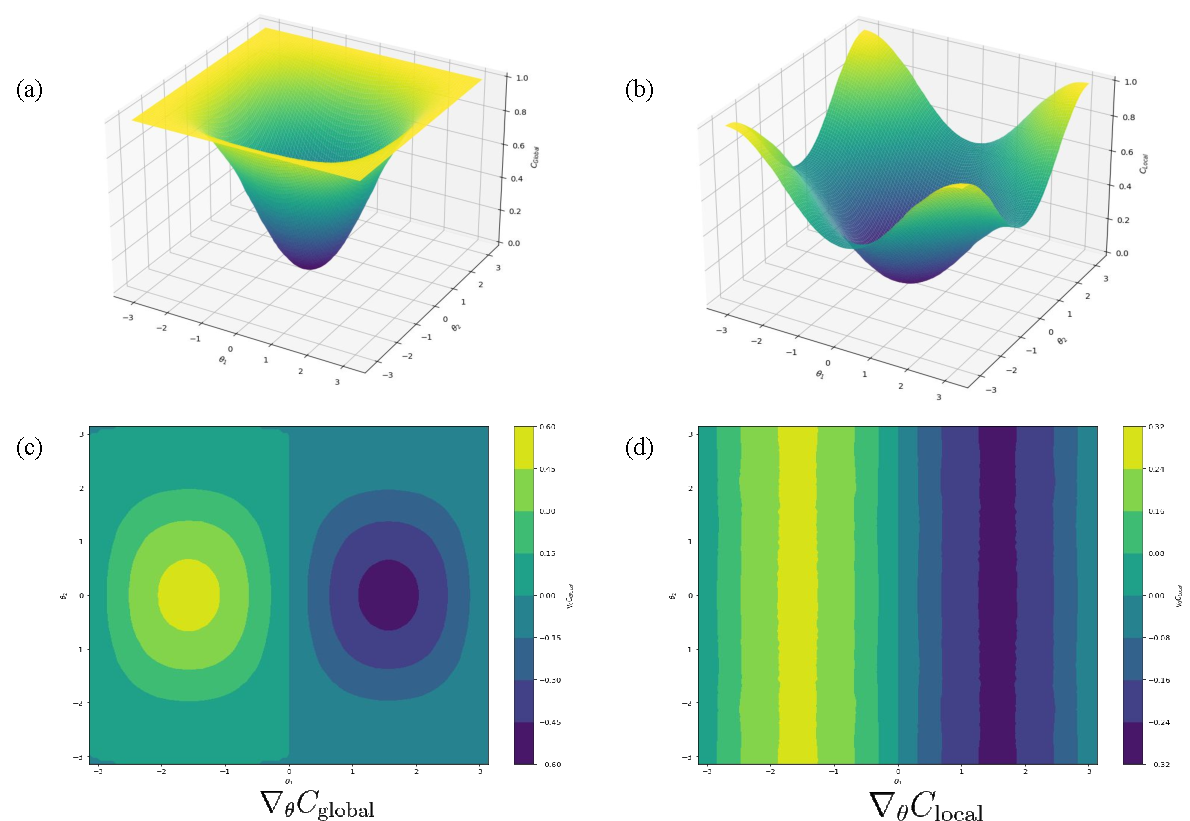
\includegraphics[width=\linewidth]{figures/qleet/barren-plateau.pdf}
%     \caption[Presence of barren plateaus in parameterized quantum circuits]{Here we show the emergence of barren plateaus in the task of learning an Identity gate using the ansatz $R_X(0,\theta_1)R_X(1, \theta_2)CZ(0, 1)$ solely based on the choice of the cost function. Figures (a) and (b) represents the loss landscape for the $\mathcal{C}_{Global}$ and local $\mathcal{C}_{Local}$ cost functions, respectively. Similarly, figures (c) and (d) represents coloured heat maps for their  corresponding gradients $\nabla_{\theta}\mathcal{C}_{\text{Global}}$ and $\nabla_{\theta}\mathcal{C}_{\text{Local}}$. We see that for $\mathcal{C}_{Global}$, the gradients vanish rapidly towards the boundaries of the loss landscape.}
%     \label{fig:barren-plateau}
% \end{figure}


\subsection{Parameter Histograms}

For our $M$-parameter PQC $\hat{U}(\vec{\theta})$, the parameters $\theta_i$ at the start of the training process are sampled from some prior probability distribution $\pi_0(\theta)$. Through the training process, we desire to learn an optimized join probability distribution over the parameters $\pi^*(\theta)$. This learnt parameter distribution
\begin{equation}
    \pi^* = \underset{\pi(\theta)}{\operatorname{argmin}} \; \underset{\theta \sim \pi}{\mathbb{E}} \mathcal{C}(\vec{\theta}) = \underset{\pi(\theta)}{\operatorname{argmin}} \; \underset{\theta \sim \pi}{\mathbb{E}} Tr[O \hat{U}(\vec{\theta}) \rho \hat{U}^\dagger(\vec{\theta})]
\end{equation}

The evolution of the parameter distribution from $\pi_0 \rightarrow \pi_t \rightarrow \pi^*$ is visualized by our parameter histogram module. The probability distributions are analyzed by starting with an ensemble of vectors $\vec{\theta_l} \sim \pi_0$, letting the entire ensemble evolve using our classical optimization subroutine, and sampling the vectors in the ensemble to get the distribution over parameters at time $t$ as $\pi_t(\vec{\theta})$. 

The marginal distribution over each variable $\pi_t(\vec{\theta_i})$ is plotted at each timestep. Change in the profile of this distribution over consecutive timesteps implies a role of those parameters in those timesteps of the learning process.


\section{\label{sec:challenges}Challenges}

In this section, we will discuss some key challenges that we come across in variational quantum computation and possible ways to identify and mitigate these problems by using tools provided in qLEET.

\subsection{Effect of Noise}

The quantum hardware that exists today are imperfect, as a result of which a computation being run on them may suffer various kinds of errors \cite{Chaudhary2022-kl}. Therefore, in order to realistically simulate and characterize the performance of a parameterized quantum circuit (PQC), we must include these errors in our computation. Our library does so by using noise models from libraries such as Cirq and Qiskit, which provides for errors related to coherent gate errors, incoherent errors, and state preparation and measurement (SPAM) errors. Users can provide the \texttt{NoiseModel} to the \texttt{CircuitSimulator} function in the simulator module while running the experiments. 

Another source of error in quantum computation arises from the limited number of times the circuit is repeatedly executed for sampling. This restricts the precision with which one can compute the Pauli observable $\hat{O}$ for calculating the cost function $\mathcal{C}$ as the number of measurements $m$ required for estimating the expectation value $\langle\hat{O}\rangle$ with precision $\epsilon$ would be $O(1/\epsilon^2)$ \cite{Higgott2019variationalquantum}. In qLEET, the default value of the number of repetitions is $1024$ and is determined by the \texttt{shots} variable, which can be provided at the time of calling any analysis function from the analyzer module.

\vspace{-2pt}

\subsection{Presence of Barren Plateaus}

The main crux of the discussion presented in the previous section is that the choice of ansatz and the cost function together is crucial for successfully training a PQC for a given task. One of the critical hindrances for the training to go as expected is the barren plateau (BP) phenomenon, where the partial derivatives $\partial_{\theta_k}\mathcal{C}(\vec{\theta})$ of the cost function $\mathcal{C}(\vec{\theta})$ with respect to variational parameters $\theta_k$ will, on average, exponentially vanish (Eq. \ref{eq:barren-plateau}). This leads to the flattening of the loss landscape, traversing through, which would require an exponentially large number of shots (for more precision) against finite sampling noise to determine the direction that minimizes the cost. Moreover, it was recently shown in \cite{2020arXiv200714384W} that BPs can also be induced due to noise present in the quantum hardware. This could be a significant issue since it could erase the potential computation advantage associated with quantum computation due to the exponential scaling required to attain the necessary precision, making the complexity comparable to classical algorithms.
\begin{equation}\label{eq:barren-plateau}
	\text{Var}_{\vec{\theta}}[\partial_{\theta_k}\mathcal{C}(\vec{\theta})] \in O\left(\frac{1}{m^N}\right),\quad \text{for}\ m > 1
\end{equation}
In qLEET, one can potentially visualize the BP phenomena by visualizing the loss landscape for a chosen PQC and cost function. This could allow users to see if BP can be mitigated by tweaking either the structure of PQC itself or just the cost function. For example, in Fig. \ref{fig:barren-plateau}, we show an example of BP dependent on the cost function in a shallow ansatz \cite{s41467-021-21728-w}. Here we compare global $\mathcal{C}_{\text{Global}}$ and local $\mathcal{C}_{\text{Local}}$ cost functions for learning the Identity gate using a very simple ansatz: $R_X(0,\theta_1)R_X(1, \theta_2)CZ(0, 1)$. 
\begin{equation}
\begin{split}
    \mathcal{C}_{\text{Global}} &= \bra{\psi(\vec{\theta})} (I - \ket{0\ldots0}\bra{0\ldots0}) \ket{\psi(\vec{\theta})} \\
    &= 1 - p_{0\ldots0}
\end{split}
\end{equation}
\begin{equation}
\begin{split}
    \mathcal{C}_{\text{Local}} &= \bra{\psi(\vec{\theta})} \Bigg(I - \frac{1}{n}\sum_j \ket{0}\bra{0}_j\Bigg) \ket{\psi(\vec{\theta})} \\
    &= 1 - \frac{1}{n}\sum_j p_{0_j}
\end{split}
\end{equation}
We see how the loss landscape flattens for the $\mathcal{C}_{\text{Global}}$ and the gradients vanish exponentially in comparison to  $\mathcal{C}_{\text{Local}}$. In addition to the BP phenomena, we also notice the narrow gorge phenomena, where global minima are contained in a steeply deep valley. This makes it difficult for gradient-based optimization to reach the global minima since it might not have a low learning rate to not overstep inside the gorge. 

\subsection{Estimation of Reachability}

Reachability quantifies whether a given PQC, $\hat{U}(\vec{\theta})$, with parameters $\vec{\theta}$ is capable of representing a parameterized quantum state $\ket{\psi(\vec{\theta})}$ that minimizes the cost function $\mathcal{C}$. Mathematically it is defined as \cite{PhysRevLett.124.090504}:
\begin{equation}
f_\text{R}=\text{min}_{\psi\in\mathcal{H}}\bra{\psi}\mathcal{C}\ket{\psi}-\text{min}_{\vec{\theta}}\bra{\psi(\vec{\theta})}\mathcal{C}\ket{\psi(\vec{\theta})},
\end{equation}
where the first and second term is the minimum over all states $\ket{\psi}$ sampled from the Haar measure and all states that the PQC can represent, respectively. The reachability is equal or greater than zero $f_\text{R}\ge0$, with $f_\text{R}=0$ when the PQC can generate an optimal state $\ket{\psi(\vec{\theta}^*)}$ that minimizes the objective function. This can be easily implemented in qLEET using the \texttt{CircuitSimulator} function present in the simulator module.  

\section{\label{sec:conclusion}Conclusion}

This paper presents an open-source library called qLEET and demonstrates its ability to analyze various properties of parameterized quantum circuits (PQCs), such as their expressibility and entangling power. We motivate the importance of studying these properties from the problem of trainability of PQCs. We have discussed and showed how important insights could be gained from visualizing loss landscapes and training trajectories for variational quantum computation. We also present the theory of expressibility and entangling capability of a PQC based on the deviation of the distribution of parameterized states produced from the Haar measure, which samples uniformly from the entire Hilbert space. We also describe the idea of the entanglement spectrum, which allows visualizing the previous two properties at once. Overall, we demonstrate how different modules included in \texttt{qleet} can be used by users to study various variational algorithms and quantum machine learning models. Finally, we discuss some critical challenges for variational quantum algorithms such as Barren Plateaus and Reachability. We conclude that qLEET will provide opportunities for the quantum community to design new hybrid algorithms by utilizing intuitive insights from the ansatz capability and structure of the loss landscape.

%--------------------------------------------------------

\chapter{Conclusions}
\label{ch:conc}
Pushing near-term quantum computers to perform useful computations that surpass the capabilities of any classical method is a daunting task, but it seems achievable through iterative progress in domains like quantum algorithm design, error correction methods, noise modeling, hardware design, and many more. In this dissertation, we have explored compilation strategies that make a small step in this direction.



%--------------------------------------------------------

%%% Optional appendix
\appendix
\chapter{qRoute: Algorithm Details and Additional Results}
\label{ch:appendix-qroute}
\section{\label{appendix:mcts}MCTS Algorithm}

The following is the detailed implementation of our MCTS procedure. In each iteration of the Monte Carlo Tree Search, we start at the root, keep selecting nodes unless we find that we have selected a node never seen before, expand it, and propagate the resultant rewards up the tree to its ancestors.

In our implementation, the value of the decay factor $\gamma$ is different for the COMMIT actions from those of SWAP actions. We use a decay of 1.0 (i.e. no decay) for the non-commit actions and 0.95 for commit actions. So we only have decay in reward propagation across 2 different states, not within the construction of a single action. The function $\textrm{step(s, a)}$ is a call to the environment to schedule the gates as described by the action $a$ and evolve the state $s_{t} \xrightarrow[]{a} s_{t+1}$.

\begin{algorithm}
	\SetAlgoLined
	\DontPrintSemicolon
	\SetKwFor{Loop}{loop}{}{end loop}
	\KwData{state $s_t$} 
	\textbf{Initialize:} root $\leftarrow$ ($s_t$, empty action set) \\
	\Loop{n\_mcts times} {
	(s, a) $\gets$ root\\
	\Repeat{last taken move was \textbf{expand}} {
		Compute \textbf{UCT} values using prior + noise \\
	    \textbf{Select} $move$ that maximizes UCT value \\
    	\eIf{(s, a).child[move] $\neq$ null} {
    	    (s, a) $\gets$ (s, a).child[move]
    	} {
    		\eIf{move $=$ COMMIT} {
    			$s^\prime$ $\gets$ \textbf{step} (s, a) \\
                $a^\prime$ $\leftarrow$ empty set
            } {
                $s^\prime \gets$ s \\
    		    $a^\prime \gets$ \textbf{insert} into $a$ the qubit pair corresponding to the move
    		}
    	    state.child[move] $\gets$ ($s^\prime$, $a^\prime$) \\
    	    \textbf{store} reward[(s, a), move] $\gets$ $\mathcal{R}$($s^\prime$, $a^\prime$) - $\mathcal{R}$($s$, $a$) 
    	}%MainIF
	}%Repeat
	    reward $\gets$ \textbf{evaluation} from model of (s, a) \\
    	\While{(s, a) $\neq$ root}{
    		p-move $\gets$ move from parent of ($s$, $a$) to ($s$, $a$)\\
    		(s, a) $\gets$ parent in tree of (s, a) \\
            reward $\gets$ reward[(s, a), p-move] + $\gamma \cdot$ reward \\
            \textbf{update} (s, a).Q-value[move] with reward \\
            \textbf{increment} (s, a).N-value[move] by 1	
    	}%While
    }%Loop
	\textbf{memorize} the Q-values and N-values at the root for training the model later \\
    (s, a)  $\gets$ root \\
    \Repeat{move $\neq$ COMMIT}{
        (s, a) $\gets$ child of (s, a) with maximum Q-value
    }
    \textbf{return} a
    \caption{Monte Carlo tree search}
\label{algo:mcts}
\end{algorithm}

\section{Results on Google Sycamore}

Following is the plot of the average Circuit Depth ratio produced by our method on the Google Sycamore processor. Sycamore has a much larger size of 53 qubits. Our method manages to give an average depth ratio of 1.64 here, and is the best of all competing routing methods.

\begin{figure}[ht]
    \centering
    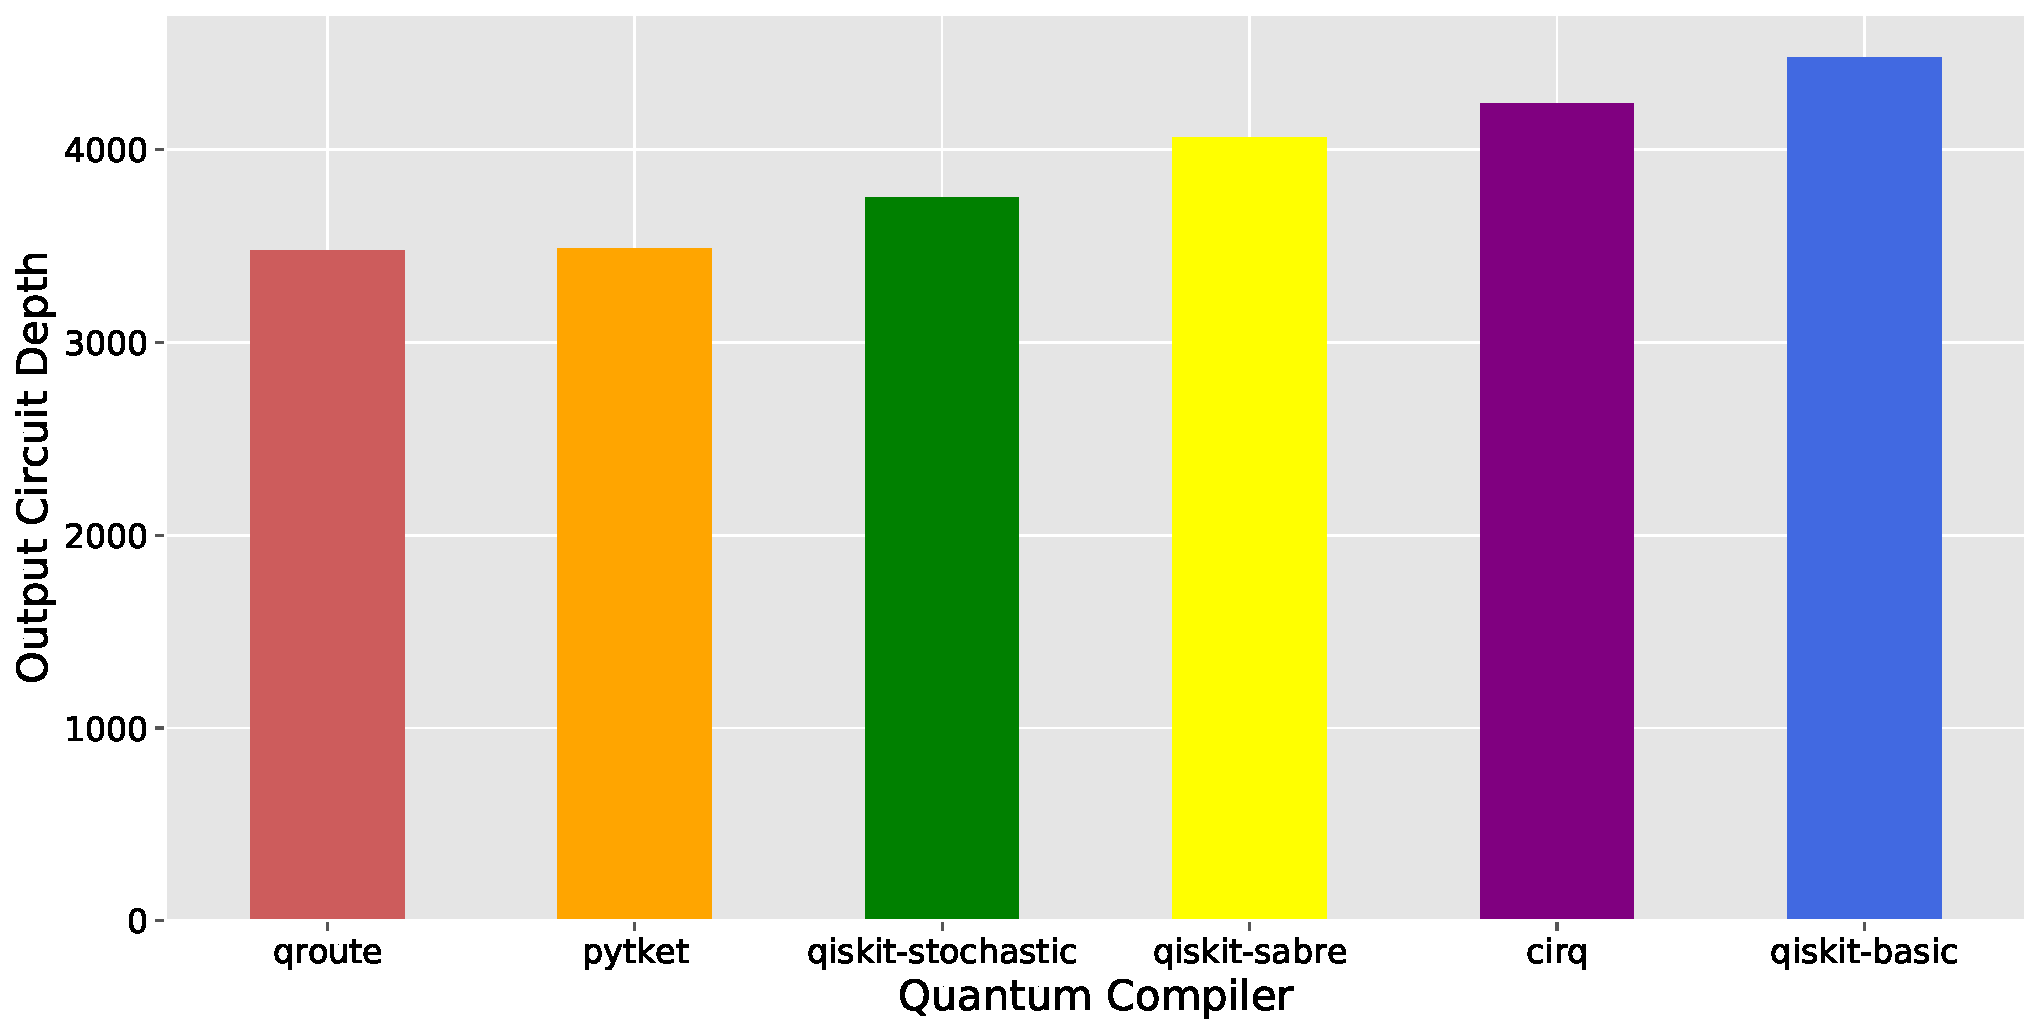
\includegraphics[width=\linewidth]{figures/qroute/sycamore.pdf}
    \caption{\label{fig:supp-sycamore-results}A comparative of the performance of the different routing methods on the small circuit dataset when routing on Google Sycamore device.}
\end{figure}

\onecolumn

\section{Example of Routing Process}

In this section, we show an example run of our algorithm on a $3 \times 3$ device with a normal grid topology, i.e. only qubits adjacent to each other are connected. In the images that follows, we have shown the evolution of the state, the value of the state at each timestep and the action, i.e. the set of gates which are being scheduled. Our MCTS is also responsible for constructing each action by putting together several moves (which are either adding individual gates to the action, or a committing the action for this timestep), that process is not demonstrated in the images. A point to note is that at the start of each timestep, the locks on all qubits may not necessarily be open, because there can be operations which were scheduled in a previous timestep and span over several timesteps. However, this is not the case in our example here where all the gates are assumed to take the same amount of time. We have provided a video simulation of this evolution as a supplementary, as well as the code to visualize this for other circuits.

\begin{figure}[ht]
    \centering
    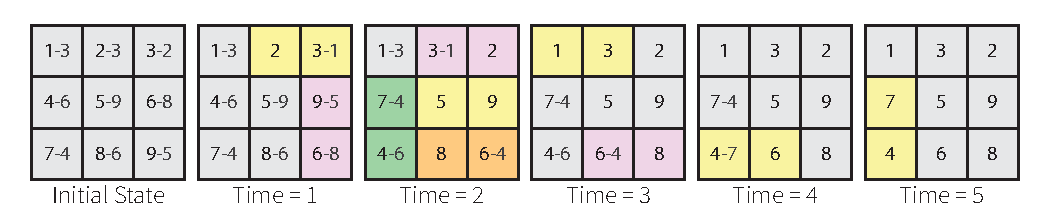
\includegraphics[width=\linewidth]{figures/qroute/Evolution.pdf}
    \caption{\label{fig:supp-evolution}The step by step evolution of the state as the circuit is getting routed. The state is shown on a $3 \times 3$ grid, where in each cell we have the node ID and the next node that it need to participate in a 2-qubit operation with. The yellow and orange colors represent that those 2 qubits have participated in a 2 qubit operation like CNOT, which was scheduled in the previous timestep. The green and purple colors represent that they have just participated in a SWAP operation. Any qubit which is colored was locked in the previous timestep when the action that scheduled it was getting constructed. At time=5, the circuit has been scheduled and none of the qubits have any targets left.}
\end{figure}

\begin{figure}[ht]
    \centering
    \hfill
    \begin{subfigure}[b]{0.38\linewidth}
        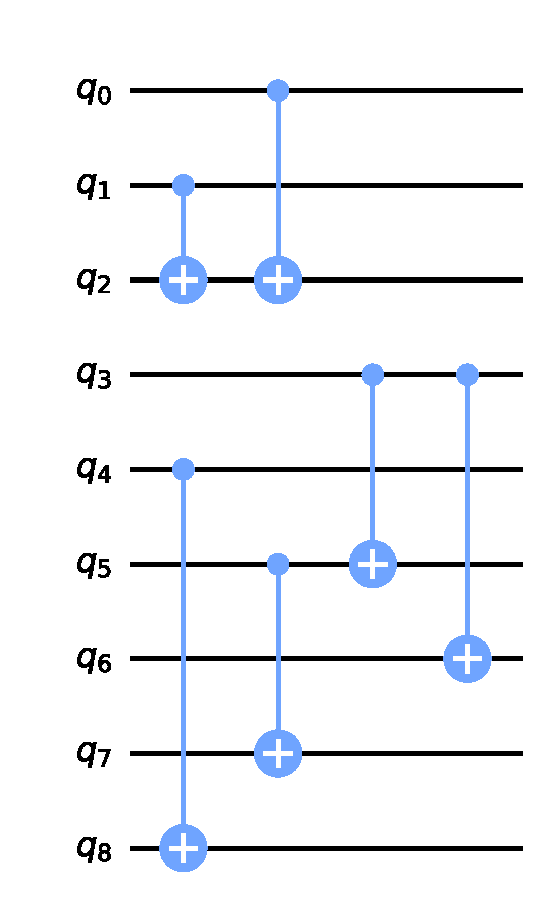
\includegraphics[width=0.7\textwidth]{figures/qroute/supp_circuit_init.pdf}
        \caption{Quantum circuit\label{fig:appendix-orig_circ}}
    \end{subfigure}
    \hfill
    \begin{subfigure}[b]{0.38\linewidth}
        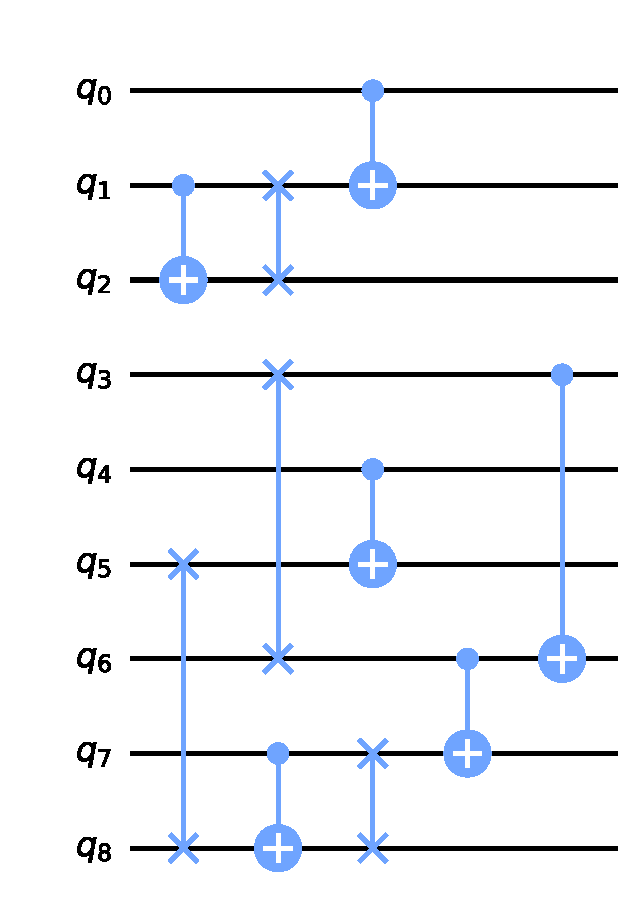
\includegraphics[width=0.82\textwidth]{figures/qroute/supp_circuit_final.pdf}
        \caption{Decomposed circuit\label{fig:appendix-sliced_circ}}
    \end{subfigure}
    \hfill
    \caption{This figure shows the input and output of the routing process shown above in Figure \ref{fig:supp-evolution}. The input circuit was used to decide the targets of the qubits. Gates are added to the output circuit whenever a 2-qubit operation, whether CNOT or SWAP is applied by the router. We can check that both these circuits are equivalent}.
    %Note that the overall unitary operation performed by the circuit is preserved despite the changes in the order of two-qubit gate operations.}
    \label{fig:appendix-routing-example}
\end{figure}

\newpage

\section{Tabulated Results}

\subsection{Random Test Circuits}

\begin{longtable}[c]{|c|c|c|c|c|c|c|c|}
\caption{\textbf{Comparative results for a set of randomly generated test circuits}}
\label{tab:random-circuits}\\
\hline
\multicolumn{2}{|c|}{Input Circuit} & \multicolumn{6}{c|}{Output Circuit Depth} \\ \hline
\# Gates      & \# Layers      & Qroute & Cirq & Qiskit (basic) & Qiskit (stochastic) & Qiskit (sabre) & t$\ket{\text{ket}}$ \\ \hline
\endfirsthead
%
\multicolumn{8}{c}%
{{Table \thetable\ continued from previous page}} \\
\hline
\multicolumn{2}{|c|}{Input Circuit} & \multicolumn{6}{c|}{Output Circuit Depth} \\ \hline
\# Gates      & \# Layers      & Qroute & Cirq & Qiskit (basic) & Qiskit (stochastic) & Qiskit (sabre) & t$\ket{\text{ket}}$ \\ \hline
\endhead
%
30  & 11 & 20 & 29  & 31  & 21  & 24  & 19  \\ \hline
30  & 11 & 19 & 36  & 39  & 23  & 27  & 28  \\ \hline
30  & 10 & 22 & 32  & 28  & 23  & 23  & 23  \\ \hline
30  & 8  & 18 & 24  & 32  & 20  & 33  & 26  \\ \hline
30  & 7  & 17 & 19  & 35  & 17  & 23  & 30  \\ \hline
30  & 11 & 18 & 39  & 34  & 22  & 31  & 26  \\ \hline
30  & 10 & 19 & 22  & 34  & 21  & 20  & 26  \\ \hline
30  & 9  & 17 & 24  & 31  & 21  & 31  & 33  \\ \hline
30  & 10 & 17 & 24  & 36  & 22  & 31  & 21  \\ \hline
30  & 10 & 21 & 23  & 39  & 22  & 27  & 23  \\ \hline
50  & 18 & 31 & 57  & 66  & 41  & 50  & 46  \\ \hline
50  & 17 & 29 & 54  & 63  & 37  & 48  & 46  \\ \hline
50  & 12 & 34 & 47  & 62  & 31  & 50  & 53  \\ \hline
50  & 17 & 28 & 62  & 67  & 38  & 38  & 58  \\ \hline
50  & 17 & 33 & 42  & 61  & 39  & 50  & 51  \\ \hline
50  & 15 & 40 & 49  & 61  & 38  & 48  & 41  \\ \hline
50  & 18 & 35 & 60  & 66  & 38  & 52  & 50  \\ \hline
50  & 18 & 33 & 54  & 53  & 35  & 42  & 52  \\ \hline
50  & 13 & 32 & 58  & 63  & 31  & 39  & 35  \\ \hline
50  & 16 & 30 & 52  & 59  & 37  & 44  & 42  \\ \hline
70  & 19 & 39 & 85  & 93  & 45  & 59  & 76  \\ \hline
70  & 21 & 47 & 96  & 71  & 41  & 56  & 60  \\ \hline
70  & 18 & 46 & 64  & 81  & 43  & 57  & 67  \\ \hline
70  & 21 & 59 & 83  & 84  & 53  & 58  & 79  \\ \hline
70  & 18 & 47 & 67  & 60  & 44  & 55  & 80  \\ \hline
70  & 21 & 45 & 77  & 83  & 46  & 69  & 59  \\ \hline
70  & 19 & 41 & 63  & 76  & 44  & 52  & 74  \\ \hline
70  & 17 & 40 & 68  & 67  & 42  & 62  & 63  \\ \hline
70  & 23 & 37 & 70  & 84  & 52  & 63  & 72  \\ \hline
70  & 23 & 40 & 64  & 91  & 49  & 73  & 60  \\ \hline
90  & 29 & 53 & 106 & 93  & 64  & 80  & 114 \\ \hline
90  & 26 & 64 & 103 & 117 & 64  & 73  & 77  \\ \hline
90  & 28 & 56 & 93  & 111 & 64  & 85  & 89  \\ \hline
90  & 22 & 57 & 94  & 114 & 54  & 75  & 87  \\ \hline
90  & 32 & 58 & 99  & 108 & 66  & 87  & 84  \\ \hline
90  & 23 & 54 & 104 & 127 & 60  & 97  & 90  \\ \hline
90  & 28 & 52 & 96  & 103 & 60  & 80  & 92  \\ \hline
90  & 25 & 50 & 97  & 113 & 60  & 76  & 75  \\ \hline
90  & 23 & 51 & 103 & 107 & 54  & 74  & 82  \\ \hline
90  & 25 & 56 & 96  & 111 & 61  & 79  & 91  \\ \hline
110 & 34 & 63 & 133 & 113 & 72  & 97  & 137 \\ \hline
110 & 27 & 65 & 128 & 143 & 70  & 95  & 118 \\ \hline
110 & 31 & 64 & 117 & 128 & 69  & 95  & 126 \\ \hline
110 & 30 & 73 & 116 & 139 & 66  & 104 & 106 \\ \hline
110 & 32 & 62 & 108 & 129 & 75  & 100 & 124 \\ \hline
110 & 36 & 68 & 112 & 135 & 78  & 93  & 107 \\ \hline
110 & 33 & 94 & 135 & 158 & 74  & 99  & 103 \\ \hline
110 & 33 & 67 & 124 & 110 & 75  & 96  & 117 \\ \hline
110 & 31 & 64 & 114 & 129 & 71  & 101 & 113 \\ \hline
110 & 30 & 65 & 116 & 145 & 69  & 97  & 115 \\ \hline
130 & 33 & 74 & 151 & 149 & 74  & 113 & 154 \\ \hline
130 & 33 & 91 & 135 & 166 & 79  & 122 & 126 \\ \hline
130 & 38 & 77 & 130 & 162 & 91  & 123 & 133 \\ \hline
130 & 32 & 77 & 112 & 153 & 75  & 116 & 139 \\ \hline
130 & 38 & 71 & 145 & 151 & 94  & 113 & 137 \\ \hline
130 & 34 & 66 & 127 & 153 & 79  & 98  & 122 \\ \hline
130 & 35 & 75 & 131 & 151 & 89  & 101 & 144 \\ \hline
130 & 31 & 70 & 114 & 157 & 74  & 107 & 135 \\ \hline
130 & 33 & 76 & 130 & 141 & 79  & 102 & 128 \\ \hline
130 & 41 & 95 & 148 & 161 & 91  & 102 & 114 \\ \hline
150 & 35 & 87 & 175 & 151 & 86  & 109 & 142 \\ \hline
150 & 44 & 92 & 194 & 195 & 104 & 154 & 158 \\ \hline
150 & 38 & 84 & 162 & 177 & 93  & 136 & 149 \\ \hline
150 & 35 & 79 & 128 & 178 & 84  & 123 & 149 \\ \hline
150 & 48 & 96 & 177 & 195 & 101 & 138 & 158 \\ \hline
150 & 43 & 92 & 179 & 167 & 97  & 126 & 142 \\ \hline
150 & 41 & 90 & 171 & 185 & 98  & 120 & 165 \\ \hline
150 & 39 & 85 & 155 & 158 & 91  & 125 & 158 \\ \hline
150 & 39 & 88 & 148 & 182 & 94  & 135 & 158 \\ \hline
150 & 38 & 89 & 178 & 162 & 96  & 123 & 159 \\ \hline
\end{longtable}

\subsection{Small Realistic Circuits}

\begin{longtable}[c]{|c|c|c|c|c|c|c|c|c|}
\caption{\textbf{Comparative results for low-depth realistic test circuits}}
\label{tab:realistic-short-circuits}\\
\hline
\multicolumn{2}{|c|}{Input Circuit} & \multicolumn{7}{c|}{Output Circuit Depth} \\ \hline
Circuit Name & Layers & DQN & Qroute & Cirq & Qiskit & Qiskit & Qiskit & t$\ket{\text{ket}}$ \\
 &  & (Estimate) &  &  & (basic) & (stochastic) & (sabre) &  \\ \hline
\endfirsthead
%
\multicolumn{9}{c}%
{{Table \thetable\ continued from previous page}} \\
\hline
\multicolumn{2}{|c|}{Input Circuit} & \multicolumn{7}{c|}{Output Circuit Depth} \\ \hline
Circuit Name & Layers & DQN & Qroute & Cirq & Qiskit & Qiskit & Qiskit & t$\ket{\text{ket}}$ \\
 &  & (Estimate) &  &  & (basic) & (stochastic) & (sabre) &  \\ \hline
\endhead
%
4gt11\_83 & 14 & 17 & 16 & 22 & 18 & 19 & 18 & 15 \\ \hline
decod24-v0\_38 & 23 & 28 & 30 & 43 & 23 & 31 & 32 & 24 \\ \hline
alu-v3\_34 & 23 & 28 & 27 & 39 & 28 & 28 & 25 & 28 \\ \hline
decod24-v3\_45 & 57 & 68 & 72 & 79 & 74 & 84 & 81 & 77 \\ \hline
4gt4-v0\_80 & 71 & 85 & 89 & 108 & 111 & 91 & 109 & 128 \\ \hline
alu-v0\_27 & 15 & 18 & 16 & 19 & 21 & 19 & 17 & 17 \\ \hline
miller\_11 & 23 & 28 & 25 & 23 & 36 & 36 & 34 & 35 \\ \hline
4gt11\_82 & 18 & 22 & 19 & 28 & 22 & 24 & 23 & 24 \\ \hline
mod10\_176 & 70 & 84 & 83 & 113 & 87 & 94 & 87 & 96 \\ \hline
ex1\_226 & 5 & 6 & 7 & 8 & 10 & 7 & 8 & 6 \\ \hline
4gt5\_75 & 33 & 40 & 38 & 54 & 40 & 41 & 46 & 43 \\ \hline
ising\_model\_10 & 20 & 24 & 23 & 40 & 20 & 20 & 20 & 5 \\ \hline
4gt11\_84 & 8 & 10 & 8 & 13 & 11 & 11 & 12 & 8 \\ \hline
4mod5-v0\_18 & 31 & 37 & 34 & 53 & 39 & 40 & 40 & 33 \\ \hline
alu-v4\_37 & 16 & 20 & 20 & 16 & 23 & 22 & 25 & 24 \\ \hline
qft\_10 & 34 & 41 & 53 & 81 & 113 & 50 & 75 & 49 \\ \hline
4mod5-v0\_19 & 15 & 18 & 17 & 25 & 20 & 19 & 24 & 26 \\ \hline
alu-v0\_27\_example & 15 & 18 & 16 & 18 & 21 & 20 & 17 & 17 \\ \hline
ex-1\_166 & 9 & 11 & 13 & 12 & 14 & 12 & 11 & 13 \\ \hline
4mod7-v1\_96 & 65 & 78 & 75 & 91 & 83 & 97 & 85 & 88 \\ \hline
4mod5-v1\_22 & 10 & 12 & 12 & 17 & 13 & 12 & 12 & 14 \\ \hline
4gt12-v1\_89 & 88 & 105 & 109 & 163 & 126 & 135 & 134 & 125 \\ \hline
alu-v1\_29 & 15 & 18 & 16 & 21 & 19 & 20 & 21 & 19 \\ \hline
mod5d2\_64 & 25 & 30 & 30 & 45 & 30 & 38 & 34 & 31 \\ \hline
4mod7-v0\_94 & 66 & 79 & 77 & 131 & 83 & 92 & 92 & 82 \\ \hline
4gt13\_91 & 46 & 55 & 53 & 64 & 52 & 68 & 60 & 52 \\ \hline
4mod5-v0\_20 & 9 & 11 & 11 & 16 & 17 & 10 & 10 & 10 \\ \hline
alu-v2\_33 & 15 & 18 & 19 & 26 & 17 & 19 & 20 & 17 \\ \hline
4\_49\_16 & 91 & 109 & 99 & 138 & 107 & 129 & 104 & 128 \\ \hline
decod24-v2\_43 & 22 & 27 & 25 & 38 & 26 & 28 & 33 & 25 \\ \hline
4gt10-v1\_81 & 60 & 72 & 71 & 113 & 82 & 80 & 81 & 75 \\ \hline
alu-bdd\_288 & 35 & 42 & 47 & 60 & 55 & 52 & 54 & 44 \\ \hline
4mod5-v1\_23 & 30 & 36 & 33 & 46 & 45 & 45 & 48 & 40 \\ \hline
one-two-three-v2\_100 & 29 & 35 & 35 & 40 & 41 & 41 & 40 & 39 \\ \hline
rd53\_138 & 42 & 50 & 54 & 70 & 67 & 69 & 78 & 59 \\ \hline
alu-v2\_32 & 64 & 77 & 72 & 96 & 88 & 87 & 98 & 96 \\ \hline
rd32\_270 & 35 & 42 & 38 & 53 & 48 & 53 & 49 & 40 \\ \hline
aj-e11\_165 & 63 & 75 & 73 & 103 & 82 & 90 & 81 & 82 \\ \hline
4gt12-v0\_88 & 77 & 92 & 90 & 128 & 116 & 111 & 107 & 140 \\ \hline
decod24-v1\_41 & 35 & 42 & 38 & 55 & 42 & 50 & 47 & 43 \\ \hline
3\_17\_13 & 17 & 21 & 24 & 17 & 26 & 18 & 24 & 22 \\ \hline
4mod5-v0\_19 & 16 & 20 & 17 & 27 & 16 & 21 & 22 & 13 \\ \hline
mini\_alu\_305 & 53 & 64 & 63 & 113 & 86 & 81 & 79 & 81 \\ \hline
one-two-three-v0\_98 & 59 & 71 & 71 & 82 & 69 & 81 & 77 & 87 \\ \hline
4gt13\_90 & 50 & 60 & 54 & 72 & 56 & 63 & 56 & 80 \\ \hline
4mod5-bdd\_287 & 31 & 37 & 41 & 48 & 35 & 48 & 50 & 35 \\ \hline
ham3\_102 & 11 & 14 & 14 & 16 & 15 & 16 & 15 & 9 \\ \hline
alu-v1\_28 & 16 & 20 & 16 & 21 & 20 & 18 & 22 & 18 \\ \hline
rd32-v0\_66 & 16 & 20 & 19 & 20 & 20 & 20 & 20 & 14 \\ \hline
cnt3-5\_179 & 43 & 52 & 64 & 91 & 72 & 61 & 65 & 83 \\ \hline
4gt13\_92 & 26 & 31 & 30 & 41 & 33 & 38 & 36 & 29 \\ \hline
alu-v4\_36 & 47 & 56 & 55 & 59 & 65 & 68 & 61 & 60 \\ \hline
rd32-v1\_68 & 16 & 20 & 17 & 21 & 20 & 20 & 20 & 14 \\ \hline
4gt13-v1\_93 & 27 & 33 & 29 & 34 & 35 & 36 & 36 & 31 \\ \hline
4gt5\_76 & 42 & 50 & 47 & 69 & 53 & 52 & 53 & 53 \\ \hline
mod5d1\_63 & 11 & 14 & 14 & 17 & 12 & 12 & 14 & 14 \\ \hline
graycode6\_47 & 5 & 6 & 5 & 9 & 5 & 5 & 5 & 5 \\ \hline
xor5\_254 & 5 & 6 & 5 & 8 & 10 & 8 & 8 & 6 \\ \hline
decod24-bdd\_294 & 31 & 37 & 34 & 50 & 40 & 40 & 46 & 37 \\ \hline
alu-v0\_26 & 35 & 42 & 41 & 62 & 47 & 48 & 45 & 54 \\ \hline
mod5mils\_65 & 16 & 20 & 19 & 21 & 17 & 21 & 25 & 18 \\ \hline
alu-v3\_35 & 16 & 20 & 20 & 25 & 23 & 21 & 21 & 24 \\ \hline
one-two-three-v1\_99 & 56 & 67 & 60 & 87 & 70 & 84 & 70 & 95 \\ \hline
one-two-three-v3\_101 & 29 & 35 & 34 & 43 & 36 & 37 & 38 & 46 \\ \hline
4gt5\_77 & 51 & 61 & 61 & 78 & 63 & 66 & 70 & 66 \\ \hline
\end{longtable}

\subsection{Large Realistic Circuits}
\begin{longtable}[c]{|c|c|c|c|c|c|c|}
\caption{\textbf{Comparative results for long-depth realistic test circuits}}
\label{tab:realistic-large-circuits}\\
\hline
\multicolumn{2}{|c|}{Input Circuit} & \multicolumn{5}{c|}{Output Circuit Depth} \\ \hline
\endfirsthead
%
\multicolumn{7}{c}%
{{Table \thetable\ continued from previous page}} \\
\hline
\multicolumn{2}{|c|}{Input Circuit} & \multicolumn{5}{c|}{Output Circuit Depth} \\ \hline
\endhead
%
Circuit Name & Number of Gates & Qroute & t$\ket{\text{ket}}$ & Qiskit (basic) & Qiskit (stochastic) & Qiskit (sabre) \\ \hline
rd84\_142 & 154 & 120 & 154 & 142 & 138 & 133 \\ \hline
adr4\_197 & 1498 & 1580 & 1770 & 1840 & 1968 & 1988 \\ \hline
radd\_250 & 1405 & 1504 & 1799 & 1812 & 1815 & 1888 \\ \hline
z4\_268 & 1343 & 1400 & 1670 & 1623 & 1718 & 1914 \\ \hline
sym6\_145 & 1701 & 1806 & 2167 & 2168 & 2261 & 2299 \\ \hline
misex1\_241 & 2100 & 2231 & 2580 & 2770 & 2681 & 2944 \\ \hline
rd73\_252 & 2319 & 2468 & 2793 & 2943 & 3071 & 3132 \\ \hline
cycle10\_2\_110 & 2648 & 2941 & 3380 & 3418 & 3485 & 3705 \\ \hline
square\_root\_7 & 3089 & 3327 & 4560 & 3759 & 3822 & 3695 \\ \hline
sqn\_258 & 4459 & 4779 & 5535 & 5526 & 5696 & 6252 \\ \hline
rd84\_253 & 5960 & 6264 & 7507 & 7411 & 7537 & 8843 \\ \hline
\end{longtable}

%--------------------------------------------------------
% Recommended 'Related Publication'
\chapter*{Related Publications}
\label{ch:relatedPubs}
\begin{enumerate}
    \item Animesh Sinha, Utkarsh Azad, and Harjinder Singh. "Qubit Routing using Graph Neural Network aided Monte Carlo Tree Search." \textit{Proceedings of the AAAI Conference on Artificial Intelligence 2022}, \textit{arXiv e-prints (2021): arXiv-2104}.
    \item Animesh Sinha, Utkarsh Azad, and Harjinder Singh. "qLEET: Visualizing Loss Landscapes, Expressibility, Entangling power and Training Trajectories for Parameterized Quantum Circuits.", \textit{arXiv e-prints (2022): arXiv-2204}.
\end{enumerate}



%--------------------------------------------------------

\bibliographystyle{style/latex8}
\bibliography{
    bibliography/main,
    bibliography/qroute,
    bibliography/qleet,
    bibliography/rlreview,
    bibliography/qalgos,
    bibliography/science
} 

\end{document}
